% IMPORT SETTINGS
% \documentclass[12pt,a4paper,twoside,openright]{report}
\documentclass{report}
% CREATED BY DAVID FRISK, 2016

% BASIC SETTINGS
\usepackage{moreverb}								% List settings
\usepackage{textcomp}								% Fonts, symbols etc.
\usepackage{lmodern}								% Latin modern font
\usepackage{helvet}									% Enables font switching
\usepackage[T1]{fontenc}							% Output settings
\usepackage[english]{babel}							% Language settings
% \usepackage[utf8]{inputenc}							% Input settings -- note: do not load this under lualatex
\usepackage{amsmath}								% Mathematical expressions (American mathematical society)
\usepackage{amssymb}								% Mathematical symbols (American mathematical society)
\usepackage{graphicx}								% Figures
\usepackage{subfig}									% Enables subfigures
\numberwithin{equation}{chapter}					% Numbering order for equations
\numberwithin{figure}{chapter}						% Numbering order for figures
\numberwithin{table}{chapter}						% Numbering order for tables
\usepackage{listings}								% Enables source code listings
\usepackage{chemfig}								% Chemical structures
\usepackage[top=3cm, bottom=3cm,
			inner=3cm, outer=3cm]{geometry}			% Page margin lengths			
\usepackage{eso-pic}								% Create cover page background
\newcommand{\backgroundpic}[3]{
	\put(#1,#2){
	\parbox[b][\paperheight]{\paperwidth}{
	\centering
	\includegraphics[width=\paperwidth,height=\paperheight,keepaspectratio]{#3}}}}
\usepackage{float} 									% Enables object position enforcement using [H]
\usepackage{parskip}								% Enables vertical spaces correctly 



% OPTIONAL SETTINGS (DELETE OR COMMENT TO SUPRESS)

% Disable automatic indentation (equal to using \noindent)
\setlength{\parindent}{0cm}                         


% Caption settings (aligned left with bold name)
\usepackage[labelfont=bf, textfont=normal,
			justification=justified,
			singlelinecheck=false]{caption} 		

		  	
% Activate clickable links in table of contents  	
\usepackage{hyperref}								
\hypersetup{colorlinks, citecolor=black, %pagebackref, %For pagebackref see: https://tex.stackexchange.com/questions/424779/can-latex-remember-from-which-page-the-user-jumped-when-clicking-on-a-reference
   		 	filecolor=black, linkcolor=black,
    		urlcolor=black}


% Define the number of section levels to be included in the t.o.c. and numbered	(3 is default)	
\setcounter{tocdepth}{5}							
\setcounter{secnumdepth}{5}	


% Chapter title settings
\usepackage{titlesec}		
\titleformat{\chapter}[display]
  {\Huge\bfseries\filcenter}
  {{\fontsize{50pt}{1em}\vspace{-4.2ex}\selectfont \textnormal{\thechapter}}}{1ex}{}[]


% Header and footer settings (Select TWOSIDE or ONESIDE layout below)
\usepackage{fancyhdr}								
\pagestyle{fancy}  
\renewcommand{\chaptermark}[1]{\markboth{\thechapter.\space#1}{}} 


% Select one-sided (1) or two-sided (2) page numbering
\def\layout{2}	% Choose 1 for one-sided or 2 for two-sided layout
% Conditional expression based on the layout choice
\ifnum\layout=2	% Two-sided
    \fancyhf{}			 						
	\fancyhead[LE,RO]{\nouppercase{ \leftmark}}
	\fancyfoot[LE,RO]{\thepage}
	\fancypagestyle{plain}{			% Redefine the plain page style
	\fancyhf{}
	\renewcommand{\headrulewidth}{0pt} 		
	\fancyfoot[LE,RO]{\thepage}}	
\else			% One-sided  	
  	\fancyhf{}					
	\fancyhead[C]{\nouppercase{ \leftmark}}
	\fancyfoot[C]{\thepage}
\fi


% Enable To-do notes
\usepackage[textsize=tiny]{todonotes}   % Include the option "disable" to hide all notes
\setlength{\marginparwidth}{2.5cm} 


% Supress warning from Texmaker about headheight
\setlength{\headheight}{15pt}		



%MELVIN settings
\usepackage{metalogo}
\usepackage{tikz} %Need to create graphs, see: https://tex.stackexchange.com/questions/270543/draw-a-graph-in-latex-with-tikz
\usetikzlibrary{arrows.meta}
\usepackage[nomarkers, nolists]{endfloat} %floats at the end of an appendix, see: https://tex.stackexchange.com/questions/129967/place-longer-figures-in-appendix/360385
\usepackage{csquotes}
\usepackage[normalem]{ulem} %strikethrough


\usepackage{color}
% \definecolor{lightgray}{rgb}{.9,.9,.9}
% \definecolor{darkgray}{rgb}{.4,.4,.4}
\definecolor{purple}{rgb}{0.65, 0.12, 0.82}

\definecolor{myred}{rgb}{0.6, 0, 0}
% \definecolor{myred}{rgb}{0.85, 0.17, 0.25}
\definecolor{bgcodegray}{rgb}{.96,.96,.96}
\newcommand{\inlinecode}[1]{\colorbox{bgcodegray}{\textcolor{myred}{#1}}}

\usepackage[export]{adjustbox} %for centering overflowing images, see https://tex.stackexchange.com/questions/16582/center-figure-that-is-wider-than-textwidth
\definecolor{mygreen}{rgb}{0,0.6,0}
\definecolor{mygray}{rgb}{0.5,0.5,0.5}
\definecolor{mymauve}{rgb}{0.58,0,0.82}

%Code listing configurations
\renewcommand{\lstlistingname}{Playlist}

%Code listing set
\lstset{ %
  backgroundcolor=\color{white},   % choose the background color; you must add \usepackage{color} or \usepackage{xcolor}; should come as last argument
  basicstyle=\footnotesize,        % the size of the fonts that are used for the code
  breakatwhitespace=false,         % sets if automatic breaks should only happen at whitespace
  breaklines=true,                 % sets automatic line breaking
  captionpos=b,                    % sets the caption-position to bottom
  commentstyle=\color{mygreen},    % comment style
  deletekeywords={...},            % if you want to delete keywords from the given language
  escapeinside={\%*}{*)},          % if you want to add LaTeX within your code
  extendedchars=true,              % lets you use non-ASCII characters; for 8-bits encodings only, does not work with UTF-8
  frame=single,	                   % adds a frame around the code
  keepspaces=true,                 % keeps spaces in text, useful for keeping indentation of code (possibly needs columns=flexible)
  keywordstyle=\color{blue},       % keyword style
  language=Octave,                 % the language of the code
  morekeywords={*,...},            % if you want to add more keywords to the set
  numbers=left,                    % where to put the line-numbers; possible values are (none, left, right)
  numbersep=5pt,                   % how far the line-numbers are from the code
  numberstyle=\tiny\color{mygray}, % the style that is used for the line-numbers
  rulecolor=\color{black},         % if not set, the frame-color may be changed on line-breaks within not-black text (e.g. comments (green here))
  showspaces=false,                % show spaces everywhere adding particular underscores; it overrides 'showstringspaces'
  showstringspaces=false,          % underline spaces within strings only
  showtabs=false,                  % show tabs within strings adding particular underscores
  stepnumber=2,                    % the step between two line-numbers. If it's 1, each line will be numbered
  stringstyle=\color{mymauve},     % string literal style
  tabsize=2,	                   % sets default tabsize to 2 spaces
  title=\lstname                   % show the filename of files included with \lstinputlisting; also try caption instead of title
}

\lstdefinelanguage{JavaScript}{
  keywords={break, case, catch, continue, debugger, default, delete, do, else, false, finally, for, function, if, in, instanceof, new, null, return, switch, this, throw, true, try, typeof, var, void, while, with},
  morecomment=[l]{//},
  morecomment=[s]{/*}{*/},
  morestring=[b]',
  morestring=[b]",
  ndkeywords={class, export, boolean, throw, implements, import, this},
  keywordstyle=\color{blue}\bfseries,
  ndkeywordstyle=\color{darkgray}\bfseries,
  identifierstyle=\color{black},
  commentstyle=\color{purple}\ttfamily,
  stringstyle=\color{red}\ttfamily,
  sensitive=true
}

\lstset{
   language=JavaScript,
   backgroundcolor=\color{lightgray},
   extendedchars=true,
   basicstyle=\footnotesize\ttfamily,
   showstringspaces=false,
   showspaces=false,
   numbers=left,
   numberstyle=\footnotesize,
   numbersep=9pt,
   tabsize=2,
   breaklines=true,
   showtabs=false,
   captionpos=b
}


% repl.it -- Lua experiments
% function replaceBacktick(input)
%   local backtickPattern = "`(..-)`"
%   local quotePattern = "`(..-)'"
%   isQuoteMatch = input:find(quotePattern)
%   if isQuoteMatch == nil then
%     print("this is not a quote")
%     print( input:gsub(backtickPattern, "\\inlineCode{" .. input .. "}") )
%   else
%     print("this is a quote")
%   end
% end


% replaceBacktick( "``the number of correctly identified instances divided by the total number of instances \cite{leong2016} '') and 2.53\% (sensitivity which``")
% replaceBacktick("`ReactComponent`")



% \usepackage{luacode}
% \begin{luacode}
% function backticks2tt ( input )
%     local backtickPattern = "`(..-)`" %This is the pattern we want to transform, provided there is no quote in between.
%     local quotePattern = "`(..-)'" %Oh no, it is a quote! Do not transform it.
%     local isQuoteMatch = input:find(quotePattern)
%     if isQuoteMatch == nil then
%         %it is not a quote, so we can try to replace it 
%         context("isQuoteMatch == nil")
%         % return ( input:gsub ( "backtickPattern" , "\\inlinecode{\\detokenize{%1}}" ) )
%         return "matched!"
%     else
%         %it is a quote, just give what it gave already and let latex handle it
%         context("matched!")
%         return "matched!"
%     end
% end
% \end{luacode}
% \AtBeginDocument{\directlua{luatexbase.add_to_callback(
%   "process_input_buffer", backticks2tt, "backticks2tt" )}}


% % Backtick program
\usepackage{luacode}
\begin{luacode}
function backticks2tt ( input )
    local isQuoteMatch = input:find("`(..-)'")
    if isQuoteMatch == nil then
        return ( input:gsub ( "`(..-)`" , "\\texttt{\\detokenize{%1}}" ) )
    end
end
\end{luacode}
\AtBeginDocument{\directlua{luatexbase.add_to_callback(
  "process_input_buffer", backticks2tt, "backticks2tt" )}}
% End backtick program
 
%both single quotes
\def\bsq#1{\lq{#1}\rq}

% % BIBLIOGRAPHY SETTINGS EXPLICITLY IN MAIN.TEX
\usepackage[style=numeric, backend=biber]{biblatex}
\addbibresource{references.bib}

% There can only be one DeclareSourcemap, see: https://tex.stackexchange.com/questions/142837/declaresourcemap-in-biblatex
\DeclareSourcemap{
  \maps[datatype=bibtex]{
    % % Need to transform howpublished field to URL field. --> https://tex.stackexchange.com/questions/311447/pdflatex-refuses-to-process-bib-file-with-hash-sign
    \map{
      \step[fieldsource=howpublished, match=\regexp{\A\\url\{(.+)\}\Z}, final]
      \step[fieldset=url, fieldvalue={$1}]
      \step[fieldset=howpublished, null]
    }
    
    % Using source maps in order to split github from other online sources
    \map{
      \step[fieldsource=url, match={github.com}]
      \step[fieldset=keywords, fieldvalue={$1}]
    }
    
    % Bold inproceedings YouTube videos, this part puts the string "important" in the keyword field
    \map{
      \pertype{inproceedings}
      \step[fieldsource=note, match={youtube.com}, final]
      \step[fieldsource=keywords, match=\regexp{\A(.+)\Z}, replace=\regexp{$1,}]
      \step[fieldset=keywords, fieldvalue={important}]
    }
  }
}

% Look at all references that have the "important" string in the keyword field and make the in-text citation bold by renewing the macro
\DeclareFieldFormat{labelnumberwidth}{\mkbibbrackets{\ifkeyword{important}{\mkbibbold{#1}}{#1}}}
\DeclareFieldFormat{boldimportant}{\ifkeyword{important}{\mkbibbold{#1}}{#1}}
\renewbibmacro*{cite}{%
  \printtext[bibhyperref]{%
    \printtext[boldimportant]{%
      \printfield{labelprefix}%
      \printfield{labelnumber}%
      \ifbool{bbx:subentry}
        {\printfield{entrysetcount}}
        {}}}}

% See: https://tex.stackexchange.com/questions/424984/biblatex-generate-which-reference-types-you-have-in-your-bib-file-for-automati
\DeclareBibliographyCategory{alreadyinbib}

\AtEveryBibitem{%
  \addtocategory{alreadyinbib}{\thefield{entrykey}}%
}

% Using source maps in order to split github from other online sources
% \DeclareSourcemap{
%   \maps[datatype=bibtex]{
%     \map{
%       \step[fieldsource=url, match=\regexp{github.com}]
%       \step[fieldset=keywords, fieldvalue={$1}]
%     }
%   }
% }


% END BIBLIOGRAPHY SETTINGS

\begin{document}
% COVER PAGE, TITLE PAGE AND IMPRINT PAGE
% \pagenumbering{roman}			% Roman numbering (starting with i (one)) until first main chapter
% % CREATED BY DAVID FRISK, 2016

% COVER PAGE
\begin{titlepage}
\newgeometry{top=3cm, bottom=3cm,
			left=2.25 cm, right=2.25cm}	% Temporarily change margins		
			
% Cover page background 
\AddToShipoutPicture*{\backgroundpic{-4}{56.7}{figure/auxiliary/frontpage_eng.pdf}}
\addtolength{\voffset}{2cm}

% Cover picture (replace with your own or delete)		
\begin{figure}[H]
\centering
\vspace{2cm}	% Adjust vertical spacing here
\includegraphics[width=0.9\linewidth]{figure/Wind.png}
\end{figure}

% Cover text
\mbox{}
\vfill
\renewcommand{\familydefault}{\sfdefault} \normalfont % Set cover page font
\textbf{{\Huge 	A Chalmers University of Technology 	\\[0.2cm] 
				Master's thesis template for \LaTeX}} 	\\[0.5cm]
{\Large A Subtitle that can be Very Much Longer if Necessary}\\[0.5cm]
Master's thesis in Master Programme Name \setlength{\parskip}{1cm}

{\Large DAVID FRISK} \setlength{\parskip}{2.9cm}

Department of Some Subject or Technology \\
\textsc{Chalmers University of Technology} \\
Gothenburg, Sweden 2017

\renewcommand{\familydefault}{\rmdefault} \normalfont % Reset standard font
\end{titlepage}


% BACK OF COVER PAGE (BLANK PAGE)
\newpage
\restoregeometry
\thispagestyle{empty}
\mbox{}


% TITLE PAGE
\newpage
\thispagestyle{empty}
\begin{center}
	\textsc{\large Master's thesis 2017:NN}\\[4cm]		% Report number given by department 
	\textbf{\Large An Informative Headline describing\\ the Content of the Report} \\[1cm]
	{\large A Subtitle that can be Very Much Longer if Necessary}\\[1cm]
	{\large NAME FAMILYNAME}
	
	\vfill	
	% Logotype on titlepage	
	\begin{figure}[H]
	\centering
	% Remove the following line to remove the titlepage logotype
	\includegraphics[width=0.2\pdfpagewidth]{figure/auxiliary/logo_eng.pdf} \\	
	\end{figure}	\vspace{5mm}	
	
	Department of Some Subject or Technology \\
	\emph{Division of Division name}\\
	Name of research group (if applicable)\\
	\textsc{Chalmers University of Technology} \\
	Gothenburg, Sweden 2017 \\
\end{center}


% IMPRINT PAGE (BACK OF TITLE PAGE)
\newpage
\thispagestyle{plain}
\vspace*{4.5cm}
An Informative Headline describing the Content of the Report\\
A Subtitle that can be Very Much Longer if Necessary\\
NAME FAMILYNAME \setlength{\parskip}{1cm}

\copyright ~ NAME FAMILYNAME, 2017. \setlength{\parskip}{1cm}

Supervisor: Name, Company or Department\\
Examiner: Name, Department \setlength{\parskip}{1cm}

Master's Thesis 2017:NN\\	% Report number given by department 
Department of Some Subject or Technology\\
Division of Division name\\
Name of research group (if applicable)\\
Chalmers University of Technology\\
SE-412 96 Gothenburg\\
Telephone +46 31 772 1000 \setlength{\parskip}{0.5cm}

\vfill
% Caption for cover page figure if used, possibly with reference to further information in the report
Cover: Wind visualization constructed in Matlab showing a surface of constant wind speed along with streamlines of the flow. \setlength{\parskip}{0.5cm}

Typeset in \LaTeX \\
Printed by [Name of printing company]\\
Gothenburg, Sweden 2017



% ABSTRACT
% \newpage
% % CREATED BY DAVID FRISK, 2016
An Informative Headline describing the Content of the Report\\
A Subtitle that can be Very Much Longer if Necessary\\
NAME FAMILYNAME\\
Department of Some Subject or Technology\\
Chalmers University of Technology \setlength{\parskip}{0.5cm}

\thispagestyle{plain}			% Supress header 
\setlength{\parskip}{0pt plus 1.0pt}
\section*{Abstract}
Lorem ipsum dolor sit amet, consectetur adipisicing elit, sed do eiusmod tempor incididunt ut labore et dolore magna aliqua. Ut enim ad minim veniam, quis nostrud exercitation ullamco laboris nisi ut aliquip ex ea commodo consequat. Duis aute irure dolor in reprehenderit in voluptate velit esse cillum dolore eu fugiat nulla pariatur. Excepteur sint occaecat cupidatat non proident, sunt in culpa qui officia deserunt mollit anim id est laborum.

% KEYWORDS (MAXIMUM 10 WORDS)
\vfill
Keywords: lorem, ipsum, dolor, sit, amet, consectetur, adipisicing, elit, sed, do.

\newpage				% Create empty back of side
\thispagestyle{empty}
\mbox{}

% ACKNOWLEDGEMENTS
% \newpage
% % CREATED BY DAVID FRISK, 2016
\thispagestyle{plain}			% Supress header
\section*{Acknowledgements}
Lorem ipsum dolor sit amet, consectetur adipisicing elit, sed do eiusmod tempor incididunt ut labore et dolore magna aliqua. Ut enim ad minim veniam, quis nostrud exercitation ullamco laboris nisi ut aliquip ex ea commodo consequat. Duis aute irure dolor in reprehenderit in voluptate velit esse cillum dolore eu fugiat nulla pariatur. Excepteur sint occaecat cupidatat non proident, sunt in culpa qui officia deserunt mollit anim id est laborum.

\vspace{1.5cm}
\hfill
Name Familyname, Gothenburg, Month Year

\newpage				% Create empty back of side
\thispagestyle{empty}
\mbox{}


% TABLE OF CONTENTS
% \newpage
% \tableofcontents

% OTHER FRONTMATTER
% List of figures (add to table of contents)
% \cleardoublepage
% \addcontentsline{toc}{chapter}{\listfigurename} 
% \listoffigures
% List of tables (add to table of contents)
% \cleardoublepage
% \addcontentsline{toc}{chapter}{\listtablename}  
% \listoftables


% START OF MAIN DOCUMENT
% \cleardoublepage
% \setcounter{page}{1}
% \pagenumbering{arabic}			% Arabic numbering starting from 1 (one)
% \setlength{\parskip}{0pt plus 1pt}

% % CREATED BY DAVID FRISK, 2016

% COVER PAGE
\begin{titlepage}
\newgeometry{top=3cm, bottom=3cm,
			left=2.25 cm, right=2.25cm}	% Temporarily change margins		
			
% Cover page background 
\AddToShipoutPicture*{\backgroundpic{-4}{40.7}{images/frontpage.pdf}}
\addtolength{\voffset}{1.5cm}

% Cover text
\renewcommand{\familydefault}{\sfdefault} \normalfont % Set cover page font
\textbf{{\Huge 	Exploring hypermedia in 2018 	\\[0.2cm]
				through the lens of XIMPEL}} 	\\[0.5cm]
{\Large Implications on parallel media, frustration detection and choice}\\[0.5cm]
Master's thesis in Master Computer Science (Multimedia specialization) 
% \setlength{\parskip}{1cm}


% Cover picture (replace with your own or delete)		
\begin{figure}[H]
\centering
% \vspace{0.45cm}	% Adjust vertical spacing here
\includegraphics[width=0.7\linewidth]{images/tom-barett_fabrizio-verrecchia_unsplash-1x.png}
\end{figure}
% There is an offset of: .2 + .5 + .5 + 1 = 2.2 so take that into consideration (e.g. 4.74 - 2.2)
% 4.74 - 0.7 
% 2 - 0.81

\vspace{-1.5cm}
{\large{Melvin Richy Roest}}
\vspace{1cm}\\
\textsc{Vrije Universiteit Amsterdam} \\
Faculty of Sciences\\ 
Amsterdam, The Netherlands 2018

\renewcommand{\familydefault}{\rmdefault} \normalfont % Reset standard font

\end{titlepage}


% BACK OF COVER PAGE (BLANK PAGE)
\newpage
\restoregeometry
\thispagestyle{empty}
\mbox{}


% TITLE PAGE
\newpage
\thispagestyle{empty}
\begin{center}
	\textsc{\large Master's thesis 2018}\\[4cm]		% Report number given by department 
	\textbf{\Large } Exploring hypermedia in 2018 through the lens of XIMPEL\\[1cm]
	{\large Implications on parallel media, frustration detection and choice}\\[1cm]
	{\large Melvin Richy Roest}
	
	\vfill	
	% Logotype on titlepage	
	\begin{figure}[H]
	\centering
	% Remove the following line to remove the titlepage logotype
	
\includegraphics[width=0.6\linewidth]{images/vu_logo.png} \\	
	\end{figure}	\vspace{5mm}	
	
	Department of Computer Sciences\\
	\emph{Section: Business Web \& Media}\\
	\textsc{Vrije Universiteit Amsterdam} \\
	Amsterdam, The Netherlands 2018 \\
\end{center}


% IMPRINT PAGE (BACK OF TITLE PAGE)
\newpage
\thispagestyle{plain}
\vspace*{4.5cm}
Exploring hypermedia in 2018 through the lens of XIMPEL\\
Implications on parallel media, frustration detection and choice\\
Melvin Richy Roest \setlength{\parskip}{1cm}

\copyright ~ Melvin Richy Roest, 2018. \setlength{\parskip}{1cm}

Supervisor and 1\textsuperscript{st} reader: Prof. Dr. Anton Eli\"ens\\
2\textsuperscript{nd} reader: Dr. ing. Sander C.J. Bakkes\\
Technical Supervision: Msc. Winoe Bhikharie\\
\setlength{\parskip}{1cm}

Master's Thesis 2018\\	% Report number given by department 
Department of Computer Sciences\\
Section: Business Web \& Media\\
Vrije Universiteit Amsterdam\\
De Boelelaan 1105, 1081 HV Amsterdam\\
Telephone +31 20 598 9898 \setlength{\parskip}{0.5cm}

\vfill
% Caption for cover page figure if used, possibly with reference to further information in the report
Cover: A visual metaphor for exploring the intersection between choice and media. The camera is cropped with the pen tool in Sketch 3. It comes from a from a beautiful photograph made by Fabrizio Verrecchia. The image in the camera is cropped from an epic background figure shot by Tom Barrett. \href{http://www.unsplash.com}{Unsplash.com} is the website where these beautiful gems have been found. The camera icons (record icon, time icon and battery icon) are made by yours truly with the marvelous pen tool. \setlength{\parskip}{0.5cm}

Typeset in \LuaLaTeX \\
Printed by Melvin's printer in his home\\
Amsterdam, The Netherlands 2018



% \newpage
% % CS (Bsc. / Msc.), Psychology of Gaming (Honours Bsc. / Msc.), International Business & Entrepreneurship (double minor), Ui/UX (200 hour bootcamp)

\section{Preface or foreword}
% https://try-dat.com Good example of a tutorial that I'd like to emulate with XIMPEL
% https://github.com/mafintosh/docker-browser-console
% https://github.com/maxogden/get-dat

% http://ximpel.few.vu.nl/
% http://ximpel.net

TO DO: Where do I add Stenzler and Eckert \cite{stenzler1996}?

For now, this is the place where I will list all my Github stuff and give people a recommendation on what to check out before reading this thesis.

% Talk about RAPT, zij doen iets met Interactive video: https://www.learningsolutionsmag.com/articles/1292/interactive-video-the-next-big-thing-in-mobile

Future work:
look for production interactive video stuff and replicate it in XIMPEL.
% https://www.mycustomer.com/experience/engagement/could-interactive-video-shape-the-future-of-customer-engagement
% http://watch.zentrick.com/m5tMjr/
% https://www.wirewax.com/examples -- via whoishiring.io
% https://helloeko.com/stories/

% For production quality: how to add nice animations? Should be its own media type?
% Nice overlay media type
% Nice overlay animations

Github:

\url{https://github.com/melvinroest/XIMPEL-JS}

\url{https://github.com/melvinroest/XIMPEL-React}

\url{https://github.com/melvinroest/ximpel-analytics-server}

\url{https://github.com/melvinroest/ximpel-terminal-media-type-server}

To checkout:

\url{http://ub-viz01.uio.no/abelprisen/}

\url{http://classic.ximpelapps.nl/zaanseschans_html5/}

To read:

\url{http://www.ub.uio.no/om/prosjekter/the-visualisation-project/news/abel-prize-app.html}

% A peculiar thing in multimedia research is that peer reviewed papers that introduced a tool are also findable on YouTube. I found these YouTube videos easier to understand and will break the tradition of scientific citation by including them in the reference lists, next to the paper.

% What is XIMPEL about? Is it about hypermedia? Is it about interactive video? A ``poor man's immersion?'' \textbf{citation needed} Or is it about gaming or education, including MOOCs? It is none of these, but it draws elements from all of these. XIMPEL is a framework that is an exploration to users. We see what users come up with and what they want to do with it, and that is what XIMPEL is.

% How is computer science science?

% Exploration 4 and 5: literature searchers are a contribution

XIMPEL is like: LaTeX is to Word. XIMPEL is a simple typesetting system but then for powerpoint.
Finite state machines are to computers. XIMPEL is a subset of everything that is computable, moreover it is multimedia.

Talk about how preserving the creative process is important

XIMPEL could be used for MOOC remixing

Hypermedia menu linking (e.g. 4 by 4 grid with videos popping up which are fully overlayed)


How is XIMPEL different from HTML? HTML has a lot of industrial support and its own namespace. But it is in essence the same: some kind of engine that renders the tags.

Take design inspiration from SMIL

----
SMIL NOTES

The only thing it did is adding the audio and video tag -- 11:10
There is a DOM API behind it
https://www.youtube.com/watch?v=xqups1sSlHI

NCL is a Brazilian spec ccitt standard. It's important for interactive tv
--> Comparable to SMIL

SMIL is all about multimedia composition.

13:46 -- What is SMIL?

Optional playback? --> opting out of media items

While watching the video it was weird to see how many thoughts I had were the same thoughts of 6 years ago.

---
Timeline is static which has a disadvantage.
The image by default plays as long as the longest thing.
--> This is handy -- Melvin: no it isn't!

XML is tractable

19:50 -- but it can be complicated (programming videos in HTML)

21:40 -- limitation of declarative hypermedia

22:10 -- interactive travel guide example

26:00 -- security updates issue and therefore the SMIL presentation didn't work anymore

Hmm... compared to SMIL XIMPEL seems like a hypermedia micro-framework

34:30 -- More use cases
Interactive Courseware (Games, quizzes)
Reactive Digital Signage (GPS-based, other environmental variables)



===
I really liked this presentation. I'm currently doing my thesis on hypermedia frameworks and seeing SMIL so well-explained really cleared a few things up, especially regarding HTML to SMIL interaction. Thanks for showing it to me. It surprises how many of the same thoughts I actually had regarding potential hypermedia features, seeing them already implemented in SMIL. I don't necessarily agree that a timeline should be omitted. Automatic synchronization is a good tool, but I think it'd be better to let the author of a SMIL presentation decide which metaphor of time to use. Yes: German does take a longer time and therefore the image could be presented longer, but what if, for some reason, the author wanted to show the image for 20 seconds regardless of the audio content length? Maybe SMIL can already do this, but it wasn't mentioned in the presentation. The assumption that video and audio control the time of images seems like video and audio have superpowers over other forms of media.

But still, it was a really interesting presentation to watch. So thanks Jack!
===

Example of a presentation: https://www.youtube.com/watch?v=FSJrrc4KF_Y
SMIL presentation (2011): https://www.youtube.com/watch?v=xqups1sSlHI 
% SMIL, Synchronized Multimedia Integration Language - Jack Jansen

Also mention DAISY: https://en.wikipedia.org/wiki/DAISY_Digital_Talking_Book
http://www.daisy.org/search/node/smil %accessibility
END SMIL NOTES
---

Hoi hoi,

Ik ben even kort aan het brainstormen. 

Stefan heeft een consequentie van zijn XIMPEL port in zijn thesis niet besproken dat misschien implicaties heeft. Dus ik wil even wat meer bewustzijn hiervoor.

In de ActionScript versie van XIMPEL kon je een XIMPEL applicatie maken. Ik neem aan dat XIMPEL gekoppeld werd via de object tag of iets dergelijks. Wat ik mij afvroeg: was het destijds mogelijk om een HTML applicatie daaromheen te ontwikkelen?

In JavaScript heeft dit sowieso een consequentie! Doordat het nu allemaal vertaald wordt naar HTML, bestaat er een mogelijkheid om de XIMPEL applicatie dynamisch aan te passen via de DOM API! Dit is niet het geadverteerde gebruik van XIMPEL, maar het kan en dat heeft grote gevolgen.

In hoeverre zou het zin hebben om XIMPEL volledig te mixen met HTML, dat wil zeggen dat je XIMPEL op zo'n manier maakt dat het een superset is op HTML, dus in feite zijn het een paar extra tags? Geeft dit ons extra nuttige mogelijkheden voor de power users?

De volgende vormen van XIMPEL zijn in principe mogelijk en ik vraag me af welke men zou willen gebruiken:
1. XIMPEL als standalone applicatie
2. XIMPEL als standalone applicatie maar met een HTML website eromheen (dit kan omdat de <body> tag er altijd omheen zit).
3. XMPEL interacterend met de JavaScript van de HTML pagina (dit kan want de huidige XIMPEL vertaald alles naar HTML5 tags)
4. XIMPEL compleet intermixend met HTML.

Met hartelijke groet,
Melvin Roest

---

First year computer science students at Vrije Universiteit Amsterdam could follow a XIMPEL command-line tutorial as their first course, without installing anything. The course itself could be implemented within a day, provided that all the artwork and written course material would be there. It is beyond me that the Vrije Universiteit Amsterdam never had a command-line tutorial in the first place when I followed courses there. Not learning the command-line early on has handicapped me in my education. Furthermore, in some computer science courses there is the problem of installing software, by having a command-line tutorial online this problem does not exist.

---

If I would be in a classroom I would raise my hand and ask: to what extent is this science? One time I did this in a computer security class and got told ``it is not science, it is engineering'' (\cite{bama2015} personal communication). What I learned from that exchange and from these papers is the following: if academics are allowed to build video browsing tools based on without regard for any theory or conceptual model other than their own intuitions as justification, I can do that too\footnote{While this could be interpreted as a critique, it can also be an acknowledgement of how difficult it can be to do science and go through the empirical cycle completely. I follow Hacker News (\url{http://news.ycombinator.com}) more or less every day and in the comments on machine learning topics it is often stated that a lot of academic deep learning papers follow more or less a similar pattern. Which is: researchers create a new architecture, it produces better results on the outcome they wanted and they have no idea why. Deep learning (and similar techniques) are not fundamentally well understood yet. And that is okay, for now. As is shown in this chapter: non-linearity is a difficult topic to untangle.}.
---



% This is all introduction!
\chapter{Introduction}
In a lot of cases groundbreaking scientific discoveries are made by accident. Without these serendipitous discoveries we would not have: penicillin, the discovery of cosmic background radiation, the microwave, X-rays, the pacemaker, matches, gunpowder, nuclear fission and the chocolate chip cookie\footnote{\url{http://mentalfloss.com/article/53646/24-important-scientific-discoveries-happened-accident} and \url{http://www.women-inventors.com/Ruth-Wakefield.asp} and \url{https://www-aps-org.vu-nl.idm.oclc.org/publications/apsnews/200207/history.cfm}}. So it begs the question should we have a plan at all? Just explore! This is a risky proposition indeed but not one without merit. 

In his book \textit{Against Method} Feyerabend argued for the idea that scientists should have a dose of theoretical anarchism \cite{feyerabend1993}. He showed that groundbreaking discoveries did not come about by adhering to a strict scientific methodology. Quite the contrary, in the case studies that he outlined all methodological principles were violated at some point. 

This is not to say that researchers are able to do whatever they want, but if exploration is a part of research, then according to Feyerabend ``anything goes'' \cite{feyerabend1993}. And in this thesis, exploration will be the biggest theme. For I (Melvin Roest) explore. For I fiddle and break things. For I acknowledge my subjective perspective and try to advance the realm of scientific knowledge. 

``What is the exploration you are on?'' you might ask. In its most simplest form I am exploring the intersection of a certain framework (XIMPEL) and its relationship to education, user profiling and hypermedia (the biggest theme). This is choice is not entirely objective. In most cases it cannot be. I study at the Vrije Universiteit Amsterdam and there is a research group developing this framework. If I would have done my Master thesis at the CWI (Institute of Informatics in The Netherlands), then I would have most likely done similar explorations with its competitor SMIL. Moreover, this choice has a component of necessity. If hypermedia and user profiling in hypermedia (and by extension the web) had been more well-documented this exploration had been more focused on (computer science) education. Alas, in order to serve education, exploring these topics is needed.

Fortunately, XIMPEL has one saving grace in which I could make it sound objective, which is: for the last 10 years XIMPEL always attempted to be at the intersection of educational games and hypermedia. It furthermore never had a logging extension for user profiling
\footnote{Though when my logging extension was complete, I discovered that another logging extension had been independently made for XIMPEL in Norway by Dan Michael O. Heggø and Huggo Huurdeman. Fortunately, the focus of both logging extensions are different enough in aim and design to be separate useful contributions.}. 
It is most likely the only framework to have had this intersection. Therefore, asking the question of: ``what is the relationship between XIMPEL and education?'' does not sound out of the ordinary. Neither does ``how does XIMPEL need to be improved for it to better serve education?'' These were the questions I started with. 
% Other questions I asked myself regarding the user profiling and hypermedia themes will reveal itself when the relevant chapters are there. I want you to explore a bit too.

In my first explorations I extended the interaction functions of XIMPEL in order to create a command-line tutorial. Would it be beneficial to make such a thing with XIMPEL compared to creating it from scratch (spoiler alert: yes)? In other explorations I simply built on future work from Stefan Bruins since it was (1) future work and (2) it was a key pillar in creating a command-line tutorial. There also were explorations in which I had a failed result relatively quickly. Yet another exploration could be seen more as traditionally academic. My penultimate exploration is entirely conceptual. And my final exploration is a showcase of hacking for future XIMPEL media type developers. Though, I have to warn you dear reader, there is a secret final exploration. After reading this thesis, would you know which one it is? Knowing it gives a hint of the thesis writing process.

On my explorations I got into more questions. Such as: ``what does interactivity mean for media and hypermedia?'' or ``is there a faster way to develop XIMPEL?'' and as a last teaser ``how could we improve the user experience of a XIMPEL presentation and make it less frustrating? Should it be less frustrating in the first place?'' These questions will be more formally introduced in each relevant chapter. 

\section{What is XIMPEL?}
Talking about a framework without explaining it does not sound like it is XIMPEL at all. It needs an explanation! More importantly, it needs a showcase. Multimedia frameworks and the like are best to be shown and explained afterwards. For the readers who never saw a XIMPEL presentation, Go to \href{ximpel.net/showcase}{http://www.ximpel.net/showcase}. The Abel Prize presentation and the tour of the Zaansce Schans presentation show various capabilities of what XIMPEL is able to do. 

Now dear reader you have a choice. To read on, or to go to the link.

What will you do?

Who said that textual media has to be linear? You can jump to a video on the web and then read on.

Click on \href{ximpel.net/showcase}{http://www.ximpel.net/showcase} if you want to see the showcase, or do nothing if you want to stay here.

If you do nothing you are missing out dear reader. Our visual cortices process information so much better than the little areas we have dedicated to purely reading.

I advice you to go to \href{ximpel.net/showcase}{http://www.ximpel.net/showcase}.

You have made your choice\footnote{In time, there will be a mirror on \href{melvinroest.com/ximpel/showcase}{http://www.melvinroest.com/ximpel/showcase}.}. We will move on.

The short explanation is that XIMPEL is a hypermedia player (linked media through overlays) or interactive video player (linked video through overlays), depending on whom is asked. The core feature of XIMPEL is that through XML, it is easy for non-programmers to play media and link it to other media by a mechanism called overlays. For example, one video is playing and there transparent square (an overlay) is in the upper right corner. A user clicks on it and another video with an image appears and both start playback from the beginning. That is the essence of XIMPEL.

When it comes to the XIMPEL framework the following stakeholders take a role in the production or consumption of a presentation. (1) the XIMPEL core developers who maintain and expand the core of the framework. (2) XIMPEL media type developers who create plugins for the XIMPEL system. It is analogous to Wordpress plugin developers. (3) The author of a XIMPEL presentation. And finally, (4) users experiencing a XIMPEL presentation.

XIMPEL its main focus is to make the lives of XIMPEL presentation creators -- also known as XIMPEL authors -- easy and simple while nudging them to become a bit computer literate. The way XIMPEL achieves this is by having an own XML specification for creating a XIMPEL presentation, known as a XIMPEL playlist. XIMPEL authors only need to know how to write this form of XML and when they do, they are able to make a presentation. It is useful in the same way that finite state machines (FSMs) are useful as opposed to a computer: the application of FSMs are limited but within that limit, it is easier to create what one wants to create.

\section{Thesis structure}
Before we move on I will introduce you to a short history of hypermedia and will explain what this is. This knowledge situates the context of what XIMPEL is, what it is not and which ideas from hypermedia are fundamental to XIMPEL. After that introduction we will move on to the explorations. For each exploration: we will first start with a short story on how I came about the idea to explore a certain topic and why it is relevant. Then I will continue to explore the topic. Each exploration will have its conclusion. After all the explorations have been presented a general discussion section concludes the thesis by summarizing it and by giving future work recommendations. 
As a last note, all the code is on my personal Github account (view the links at \cite{github:ximpel_react, github:ximpel_js, github:ximpel_analytics_server, github:ximpel_terminal_media_type_server}). 

% When one thinks about this a bit, one might wonder how a non-interactive artifact such as media could possibly intersect with an interactive artifact such as digital games. This is because \textit{hypermedia is interactive!} In short, hypermedia is media  with hyperlinks. Just like hypertext is text -- a form of media -- with hyperlinks. HTML5 has a lot of hypermedia functionality, HTML4 did not.


% \subsection{The need for hypermedia in education}
% A system like this allows users to deal with complex information. ``Reality is intertwinkled.'' 

% A hypermedia system is good for describing linear and non-linear relationships between media content. One recurring theme for hypermedia is using it for education. %cite this as a motherfucker
% A specific use case for that is for visual displays in museums. Another more generic use case is almost any slide show presentation.
% % TO DO: do all the comments!

\chapter{A brief Amsterdam-centric history of hypermedia}
% Why hypermedia is important (next 3 paragraphs)
The research area that the XIMPEL framework connects with or situates itself in are: education, game-design, narrative structure, interactive video and hypermedia. There might be more areas, but previous research regarding XIMPEL has been around these areas \cite{eliens2008, eliens2016, eliens2007, stefan2016}. A chapter published in 2016 about XIMPEL is called:``XIMPEL for Education -- inspiring creativity through storytelling and gameplay.'' Furthermore, XIMPEL presentations themselves demonstrate that they are a form of interactive video. A user is able to click on overlays and then jumps to another video which could be part of a narrative. Interactive video is a part of hypermedia and since more media items are able to be linked in XIMPEL one could argue that XIMPEL itself is a hypermedia framework or at the very least heavily inspired by one.

Because of this it is of utmost importance to describe this field. Hypermedia is the research field where fundamental questions regarding XIMPEL lie. Without the ideas of hypermedia, and by extension ideas surrounding the world wide web, there would be no XIMPEL. By portraying the historical roots, any reader is able to have an idea of how this research field has developed. On another note, to a certain extent, the research field of interactive video is implicitly described a little bit as well since it is part of hypermedia.

Education, game-design and narrative structures are research fields of their own that are more into connection with XIMPEL than the context of XIMPEL. This is because it is possible to create presentations or applications with XIMPEL that may show unexplored topics of research within these areas of research. Since not all XIMPEL presentations or applications are subsumed under these research fields, they will not be described from a historical perspective. There where it is needed, research from these areas will be used as reference.

%Define hypermedia (if easy, otherwise don't) -- currently don't
%https://en.wikipedia.org/wiki/Hypermedia misschien inspiratie?
\section{What is hypermedia}
Hypermedia is to media what hypertext is to text. Moreover, text is a form of media. The idea of hypertext itself is confusing since it can be seen as (1) text with links or (2) the HTML specification. HTML is a markup language for hypertext, but there are also images and since HTML5 also videos and audio. It could be argued that HTML5 has hypermedia elements, much more so than the earlier versions of HTML. The conceptualization of hypermedia started in the early 90's, and during that time HTML was purely meant for (hyper)text\cite{html1}. Hence, the first definition of hypertext seems to be the intended definition by the authors of the early 90's. So a hypermedia system can be viewed as a system that is able to display all forms of media and all forms of media can be linked to each other in the way that users are nowadays familiar with the web (e.g. by tapping or clicking on areas that link to some other form of media).

Regarding the implementation of a hypermedia system it needs to have 3 components: (1) a description of its media components, (2) a way of defining relationships between media components such that they are connected and (3) a way of presenting these components on the computer screen. Media components could be blocks of text, animations, audio, video and user-defined media components. Links describe the relationships between media component. The idea of linking could be defined in a number of ways. The presentation can be determined by the hypermedia system itself through a rendering system. 

Specifically for XIMPEL these 3 components have been realized by using web technologies. (1) the description of media components are described in XML within a document called the playlist, (2) overlays (hovering rectangles or other shapes that are clickable) can be laid over the media item playing within XIMPEL and when clicked, it stops the current media playing item and plays the media item that the overlay links to. (3) The Flash player used to be the rendering engine of XIMPEL. Nowadays, it is the browser for which HTML5, CSS and JavaScript are needed regarding the rendering process.

%For a quick overview see: http://www.cyberartsweb.org/cpace/ht/christanto/dexter_model.htm
%Difference between WWW and Dexter: http://www.shlomifish.org/humour/fortunes/show.cgi?id=tim-berners-lee-the-WWW-and-the-dexter-model

%The WWW and the Dexter Model
%https://en.wikipedia.org/wiki/Ted_Nelson misschien erbij?
% http://paul.luon.net/hypermedia/chapter6/modelsFrameworks/dhrm.html
% \section{The Dexter Hypertext Reference Model}
%The Dexter Model and What were their methodologies?
Research in hypermedia has been conceived by research on hypertext systems. Most notably, the Dexter Hypertext Reference Model has been influential in the development regarding popular hypermedia concepts \cite{hardman1994}. It has been a competing against the hypertext model of Tim Berners-Lee who created the world wide web as we know it today. The model itself came into existence after two small workshops on hypertext, which had representative participants for most major hypertext systems made during that time. Halasz, Schwartz, Gr{\o}nb{\ae}k, Kaj and Randall remarked that the model ``is an attempt to capture, both formally and informally, the important abstractions found in a wide range of existing and future hypertext systems'' \cite{halasz1994}. 

%What is it?
%Insert figure or create yourself -- currently don't
The Dexter Hypertext Reference Model (hereafter Dexter Model) has three layers: the run-time layer (user interaction mechanisms), the storage layer (a network of nodes and links to those nodes) and the within-component layer (content and structures within hypertext)\cite{halasz1994}. A big difference compared to the world wide web today is that links needed to resolve both ways \cite{fisher2007}. If this was not the case, then if one hypertext component was deleted, every hypertext component linking to it would need to delete its link. 

%How is it relevant for hypermedia?
% The relevance of the Dexter Model to hypermedia to date is the methodology of its conception. By looking at the most well-known hypertext systems of then, summarizing them and discussing them with peers a technical vocabulary has been created. The methodology and academic relevance for the use of XIMPEL will be inspired by this manner of motivating the academic relevance of a system. Furthermore, the Amsterdam Hypermedia Model, which is the most influential model on hypermedia, took the idea of the hyperlink and combined it with their pre-existing media model: the CWI Multimedia Interchange Format.



%file:///Users/melvinroest/Downloads/The_Amsterdam_Hypermedia_Model_Adding_Time_and_Con.pdf
\section{The Amsterdam Hypermedia Model}
The Dexter Model gave rise to the predecessor of what was going to be the most popular hypermedia framework for about twenty years: The Amsterdam Hypermedia Model. The underpinnings of it eventually became a W3C recommendation in the form of SMIL \cite{ossenbruggen2001}. It began by addressing the limitations of the Dexter  Model for describing hypermedia. Hypertext and hypermedia are not the same so it seems obvious that these limitations should exist. Hardman and Bulterman stated that ``it has no notion of time beyond the within-component layer,'' \cite{hardman1994} such as the Dexter Model has and further stated it has ''no way of specifying higher-level presentation information, and no notion of context for an anchor'' \cite{hardman1994}. Context here means: does the whole presentation change or just a part of it? At the time their own media model, the CWI Multimedia Interchange Format (CMIF), had the drawback that it did not specify links but did address the other issues that the Dexter Model had. The solution was taking inspiration from both and it could be argued that The Amsterdam Hypermedia Model in its shortest (and not fully accurate) description is the combination of CMIF with linking capabilities inspired by the Dexter Model. 

The Amsterdam Hypermedia Model (AHM) is about combining multimedia in such a way that it forms a presentation in which there is the possibility of (non-linear) choice at certain moments. For example, one could watch a penguin video, see a header text penguins and then be presented with the choice to let them dance or to let them walk a bit more. One could then interact with the video by stating the choice and then a subsequent video with new header text would be displayed. We will now look on what the elements of the AHM are that allow us to create such a multimedia presentation.

%synchronization (timing relations)
%composition: A slight change to composition in the Dexter model is the removal of the contents for a composite component. We restrict the presence of contents (data blocks in the CMIF model) to atomic components. This gives a cleaner notion of composition and removes complications about where the contents exist in the presentation hierarchy— they are always at the leaf nodes.
%Atomic component: can contain static media (image) or dynamic media (video)
%Composite component can be: parallel or choice -- choice means that one of the children is played

\subsection{Components}
The AHM has multimedia resources which can be an image, text, video or music. These resources are called atomic components. The other component is a composite component which can either be a component that plays atomic components in parallel or a component that allows the user to select one atomic component to be played. These are two respective types (parallel or choice) of the parallel component. This design feature is \sout{stolen} direct inspiration regarding parallel media play in XIMPEL (see chapter \ref{chap:exploration2}).

% Figure 7. Timing relative to sibling
% (a) Children start at the same time.
% (b) Right-hand child starts with a specified delay after left-hand child. (c) Right-hand child starts after left-hand item ends.
% (d) Children end at same time.
%Synchronization arcs are needed for atomic media items that are not siblings

%About time
% What is a Sync-arc?
% When one element defines a begin or end time relative to the begin or end of another element. 
% img begin="foo.begin" end="bar.end" ...
% Creates an additional 'arc' in the timegraph
% Defines a time dependency
% 'Short' and 'long' sync arcs
% Define timing, not runtime sync!

% Sync-arcs & time dependents
\subsection{Time}
The AHM had a way of defining time relationships between siblings and children in a parallel component in the form of synchronization constraints. These constraints are necessary, otherwise no one knows when something ought to be played. The AHM also has the capability to define time relationships between different (non-family) components via synchronization arcs, which are optional. An example of a synchronization arc is when a video plays, then it is optional to have subtitles but if subtitles are played, then they need to start 5 seconds later than the video.


% In the Amsterdam hypermedia model, channels are used to define a default presentation style for the atomic com- ponents which are played via that channel. Channels are defined globally (for a collection of documents) and are referenced by each atomic component. A channel applies to only one media type. A number of channels may be appropriate for any one atomic component. Only one atomic component can occupy a channel at any one time.
\subsection{Channels}
How is certain media presented? Is there space for a menu? How does that look like when a video is played? Can a video play full screen when there is a menu? These questions are all about the general styling of a multimedia presentation. To answer these questions, the AHM introduced the idea of channels. Channels are ``output devices for playing multimedia items'' \cite{hardman1994}. Channels play an atomic component, for example: one channel could be playing videos, whereas another channel would display text. It is not possible for a channel playing videos to also play text. Also, a channel can only play one atomic component at a time. Examples of channel definition are: the default font size, size of the window, z-index layers, and position of the multimedia element (atomic component). One could already imagine that generic layouts are a good use case for channels since channels are reusable.

%Link context is interesting
%A link introduces the concept of choice

\subsection{Links}
Since the Dexter Model is different than the current model of the world wide web, the idea of links here are slightly different as well. A link in the AHM can have a context. A link context allows for specification for which part of the document needs to change. Specifying a link context has the idea that when a presentation changes, it only changes what it needs to change, allowing for reusability of the components in the AHM. Links ought to be clicked, and therefore links introduce choice. For this reason, the choice component is an obvious but necessary requirement.
% In the web-development world contextual links are now in production through JavaScript frameworks such as ReactJS by defining React components (React also has a concept which they call components).

%CREATE EXAMPLE DIAGRAM OR STEAL IT -- example diagram of what? -- currently don't



%Paper with SMIL Editor: https://homepages.cwi.nl/~dcab/PDF/WWW7.pdf
%https://homepages.cwi.nl/~media/SMIL/Tutorial/SMIL-4hr.pdf
% http://www.cs.vu.nl/~eliens/demo/2-2.html
%https://www.w3.org/standards/techs/smil#w3c_all
\section{SMIL}
``Most constructs in CMIF and SMIL are explicitly modeled by the Amsterdam hypermedia model'' \cite{ossenbruggen2001}. Therefore, SMIL could be seen as the successor of the proposed AHM. SMIL has been the standard on synchronized multimedia until 2013. While SMIL has been supported by a lot of well-known companies, it has not been supported by all of them. Unfortunately, the SMIL working group disbanded and SMIL is not updated anymore\cite{smilStatus, smilStatus2}. Moreover, future ideas of SMIL seem not to be included as a standard, such as Time Style Sheets \cite{timestylesheets2014}. It seems that HTML5 bares the burden of bringing hypermedia to the masses \cite{smilStatus2}, albeit much less feature rich. An example of a SMIL presentation can be found here \cite{SMIL_example} and a lecture about SMIL 3.0 and how the XML tags look like can be found here \cite{SMIL_lecture}. Current SMIL presentations need an external player or browser plugin.

\section{XIMPEL}
In 2007 a new hypermedia framework started called the eXtensible Interactive Media Player for Entertainment and Learning \cite{eliens2016, eliens2008}, or in other words: XIMPEL. It was created in order to design a game about climate change. The goal was to lead the debate away from pathos (emotional arguments) and towards logos (logical arguments) \cite{eliens2007, eliens2008}. Before XIMPEL was conceived, the idea was to create an immersive game with the Half-Life SDK about climate change. However, it seemed infeasible because of too few resources. Therefore, the team created the XIMPEL framework and decided to created a game purely based on videos still allowing for what they called a \textit{poor man's immersion}. 

Borrowing ideas from hypermedia for game development was perhaps overlooked at the time since hypermedia formats -- including its platforms -- such as SMIL were focused on a good structure of hypermedia. Where probably most (if not all) hypermedia platforms focused on the formalities of a hypermedia system. The XIMPEL platform focused on exploring possible applications. XIMPEL was created out of necessity for an educational game that would otherwise take a long time to make. From this perspective, XIMPEL should be compared to game development engines and it is one of the most unconventional game development engines in existence.

Over the years the framework has evolved from its Flex SDK/Flash roots to a HTML5/JS/CSS version. One creator (Anton Eli\"ens) of XIMPEL taught every year how to use it to first year information science students\footnote{I was a student in one of these years}. These students created at least one presentation with it in a group of 2 or 3. In some cases, students ran into technical problems and either extended XIMPEL themselves or through the help of Winoe Bhikharie. By doing this Anton and Winoe unwittingly explored the question: what can hypermedia mean for serious games? Moreover, what hypermedia presentations are relevant and interesting? While XIMPEL is a hypermedia system, the questions explored with it are about serious games and non-linear narratives. 

% Touch screen applications
Current future work regarding XIMPEL is expanding the framework for usage of big tablet installations at museums. One example of that is an app made for the Abel Prize, which is a prestigious prize for mathematicians \cite{abel_prize}. Workshops are given in Norway to librarians for whom the XML format is easy to work with. 

So XIMPEL is useful for:
\begin{itemize}  
    \item education,
    \item prototyping digital games,
    \item video narratives/interactive storytelling,
    \item storyboarding,
    \item big tablet installations
\end{itemize}

% Explain how XIMPEL works?

% http://www.fxpal.com/publications/synchronizing-web-documents-with-style.pdf -- Bulterman 2014 Time Style Sheets
\section{Now}
Hypermedia is still here. One of the creators of SMIL (Dick Bulterman) asked himself how the ideas he knows from SMIL could be useful for CSS. He  proposed additional CSS attributes to the W3C \cite{timestylesheets2014}. Hypermedia and hypervideo systems have been ported to HTML5/JS/CSS and are still used today \cite{meixner2016, celentano2017, busson2017}. 

All systems have their own unique spin on it. Some emphasize videos  \cite{meixner2016} or mix it with it with other ideas of software engineering (e.g. learning objects) \cite{busson2017}. Others focus on hypermedia systems \cite{celentano2017}. 

To clear out confusion, this thesis is not about hypermedia APIs. A concept in API-design that allows for REST-based APIs that are more robust. For example, it is easier to avoid backwards compatible breaking changes compared to standard REST API-design.

% ask yourself what you want to do here -- talk about the changing role of hypermedia I suppose
% Footnotes here are fine
With the advent of HTML5 the role of hypermedia will be different. Considering an HTML document merely as a document and not as a possible software application would be short-sighted. Thanks to JavaScript it is possible to create: Linux in the browser \footnote{\url{https://bellard.org/jslinux/vm.html?url=https://bellard.org/jslinux/buildroot-x86.cfg}}, create a programmable computer through the Game of Life \footnote{\url{https://codegolf.stackexchange.com/questions/11880/build-a-working-game-of-tetris-in-conways-game-of-life}} or create anything else that one could imagine. In short, it used to be very difficult to create any application -- requiring technologies like Flash. Now this is not the case anymore.

% Search for extra literature regarding hypermedia now

% Talk about companies that do hypermedia


% \chapter{Explorations}
Now that we have some idea of where the philosophical forefathers of XIMPEL came from it is time to explore! The conscious choice of having no methodology has been informed by the philosopher Feyerabend. There are two starting questions. These are: what is the relationship between XIMPEL and education? And how does XIMPEL need to be improved for it to better serve education? 

The idea of the explorations are that once an exploration is done, it may give rise to other questions that need to be explored. One exploration question came up by daydreaming about XIMPEL, this is exploration 4. I took a course in user experience design and realized how important a good user experience is. During my time as a student I noticed that a lot of students experienced frustrating moments while experiencing a XIMPEL presentation. It begged the question: is it possible to (semi)automatically detect user frustration within XIMPEL presentations? One assumption is that this type of detection may help the user experience for XIMPEL presentations. The chain of how one exploration caused another exploration happened as follows: exploration 1 (from the starting questions), exploration 2 (from exploration 1 and from the starting questions), exploration 3 (from exploration 1), exploration 5 (from exploration 2) and exploration 6 (from exploration 2). For some preservation of the creative context: what went through my mind will be a short story per exploration as the first few paragraphs.

Among other things, explorations have one key difference with experiments in that they are unfortunately not reproducible. This is a blessing and a curse. It is a blessing because I have encountered zero papers (!) that reported the reproduction of a result of another computer scientist. It is a curse, because I am admitting that a certain form of objectivity is lost. To be fair, many papers in computer science seem not to be reproducible because not enough information is presented in order to recreate a proposed system. And the nature of the field gives the impression that engineering replaces science. One could argue that working technology is a certain truth on its own, which is what science is about.

% Since I already outlined the history of XIMPEL I can answer the first question, which I will 
% The relationship between XIMPEL and education can be seen from its entire history starting from the beginning. Wanting to educate 

The non-reproducibility is not how this body of work in this thesis is relevant. Fortunately, there are other ways to contribute towards the academic discussion for any given topic. A few examples are: creating tools, new relevant examples of application regarding a particular system or simply asking questions that have not been asked but which are relevant. In the following paragraphs the specific contributions per exploration are stated.

\textbf{In exploration 1} The implementation regarding the creation of a command-line tutorial in XIMPEL is presented. The contribution of this exploration is showing the boundaries of XIMPEL when a developer discards the hypermedia ideal and solely focuses on education. The implementation of the command-line tutorial itself is a contribution to the XIMPEL framework, including its programmed server. Moreover, there is an attempt to answer the question: when is something hypermedia and when is it not?

\textbf{In exploration 2} the future work that was presented in the thesis of Stefan Bruins\cite{stefan2016} which is creating a parallel player for XIMPEL. Bruins focused on the main question whether the XIMPEL framework could be implemented with HTML5, CSS and JavaScript. In this exploration I focus on the question on how to architect and implement a parallel media player within XIMPEL. The contribution is an implementation and architecture overview of a parallel media player. Furthermore, the a parallel media player in XIMPEL creates new questions such as: what if a media item survives a subject switch (called media item subject switch survival, i.e. MISSS)? Or: how does one do timescrubbing in XIMPEL? These questions are explored in a new exploration.

\textbf{In exploration 3} I assess whether XIMPEL can be recreated with ReactJS (a front-end JavaScript library created by Facebook) in an effective manner. In this exploration I successfully and unsuccessfully recreate XIMPEL with ReactJS as opposed to plain JavaScript and jQuery. The contribution of this is most of XIMPEL recreated in ReactJS and a relative full description of the creative process of getting there. It furthermore, implements ideas from almost all explorations and has ended as a recreation of XIMPEL and also as my vision for XIMPEL, which is more web-based than the current version. For the attentive reader this is secretly both exploration 3 and the final exploration because of the messy timeline.

\textbf{In exploration 4} I explore how to (semi)automatically detect frustration of users within XIMPEL presentations. The contribution of this exploration is an implemented logging extension for XIMPEL. The logging extension captures: facial expressions, mouse clicks, mouse moves and the history of what the user already has seen. There is furthermore a conceptual description on how to detect frustration specifically for the XIMPEL framework.

\textbf{In exploration 5} I wanted to implement a time-scrubbing mechanism, but slowely and surely I realize that there are many twists and turns when it comes to time-scrubbing in hypermedia applications! It suffices to say that architecting and implementing time-scrubbing for single videos is much more straightforward than multiple videos (and other forms of media) that share a certain relationship with the other media elements. The contribution of this exploration is an analysis of which design choices one could possibly take in order to create time-scrubbing in XIMPEL. Analyzing these design choices was equally rooted in: literature, rationality and imagination.

\textbf{In exploration 6} In short story form I write about how I extend XIMPEL with one extra parameter in a method definition and show how this extension can lead to some serious media type hacking for media type developers. To showcase this, I implemented a YouTube media type that does not immediately detach from the DOM when a new subject is clicked on. The contribution of this exploration is: (1) the introduction of a new concept -- partial media type refreshes, (2) a showcase on extending media types so that this functionality becomes available and (3) an implemented YouTube media type that supports partial refreshes.

% Afsluitende alinea? Structuur per exploration
In closing, the structure of any exploration is as follows:
\begin{itemize}
    \item short story what went through my mind
    \item introduction to exploration
    \item the exploration itself
    \item conclusion and future work
\end{itemize}

% \chapter{Exploration 1: creating a command-line tutorial in XIMPEL}
\label{chap:exploration1}
Looking at the structure of many MOOCs, it could be observed that they all have a simple video playlist and then follow up with some multiple choice questions or a coding assignment within an online code editor. Is it not possible to recreate a command-line tutorial with XIMPEL? Because if it is, then it will be a lot quicker to create such an application compared to creating it from scratch!

On a related matter, with the implementation of a command-line tutorial, XIMPEL could compete with computer science courses on Coursera. It could not compete on design but on pragmaticism, not on flexibility but on programming simplicity, not on comprehensiveness but on development speed. With this extension, XIMPEL occupies a unique niche of hypermedia and education.

By recreating a command-line tutorial in XIMPEL I stumbled upon a question. A command-line interface is not a form of media. A command-line interface is an application. So by recreating this in XIMPEL I am mixing a computer application with hypermedia. What does this mean? Am I now leaving hypermedia? Are we mixing hypermedia elements with a computer application? Could XIMPEL still be considered a hypermedia framework? Should XIMPEL be a hypermedia framework in the first place? 

The questions that I will formally focus on in this exploration are: how would XIMPEL need to be extended in order to create a command-line tutorial? And what are the implications of mixing a hypermedia application with another (non hypermedia) application with regards to hypermedia as a field?

\section{Extending XIMPEL to create a command-line tutorial}
Did you know that the XIMPEL is an acronym for eXtensible Interactive Media Player for Entertainment and Learning? Neither did I at one point. The extensibility of this media player will be demonstrated here. Together with the core changes I made in the framework, it is even more extensible!

So is it possible to recreate a command-line tutorial with XIMPEL? The answer is yes. Our research question has been answered. I suppose we are done.

Which command-line tutorial are we recreating you might ask? From CodeCademy\footnote{\hyperlink{https://www.codecademy.com}{https://www.codecademy.com}} of course! It is one of the leading organizations for online programming education. To give a feel for how CodeCademy looks like I recommend you to try the command-line tutorial yourself. For readers who are reading this on paper, figure \ref{fig:codecademy} will show a screenshot from a part of the command-line tutorial.

\begin{figure}
    \centering
    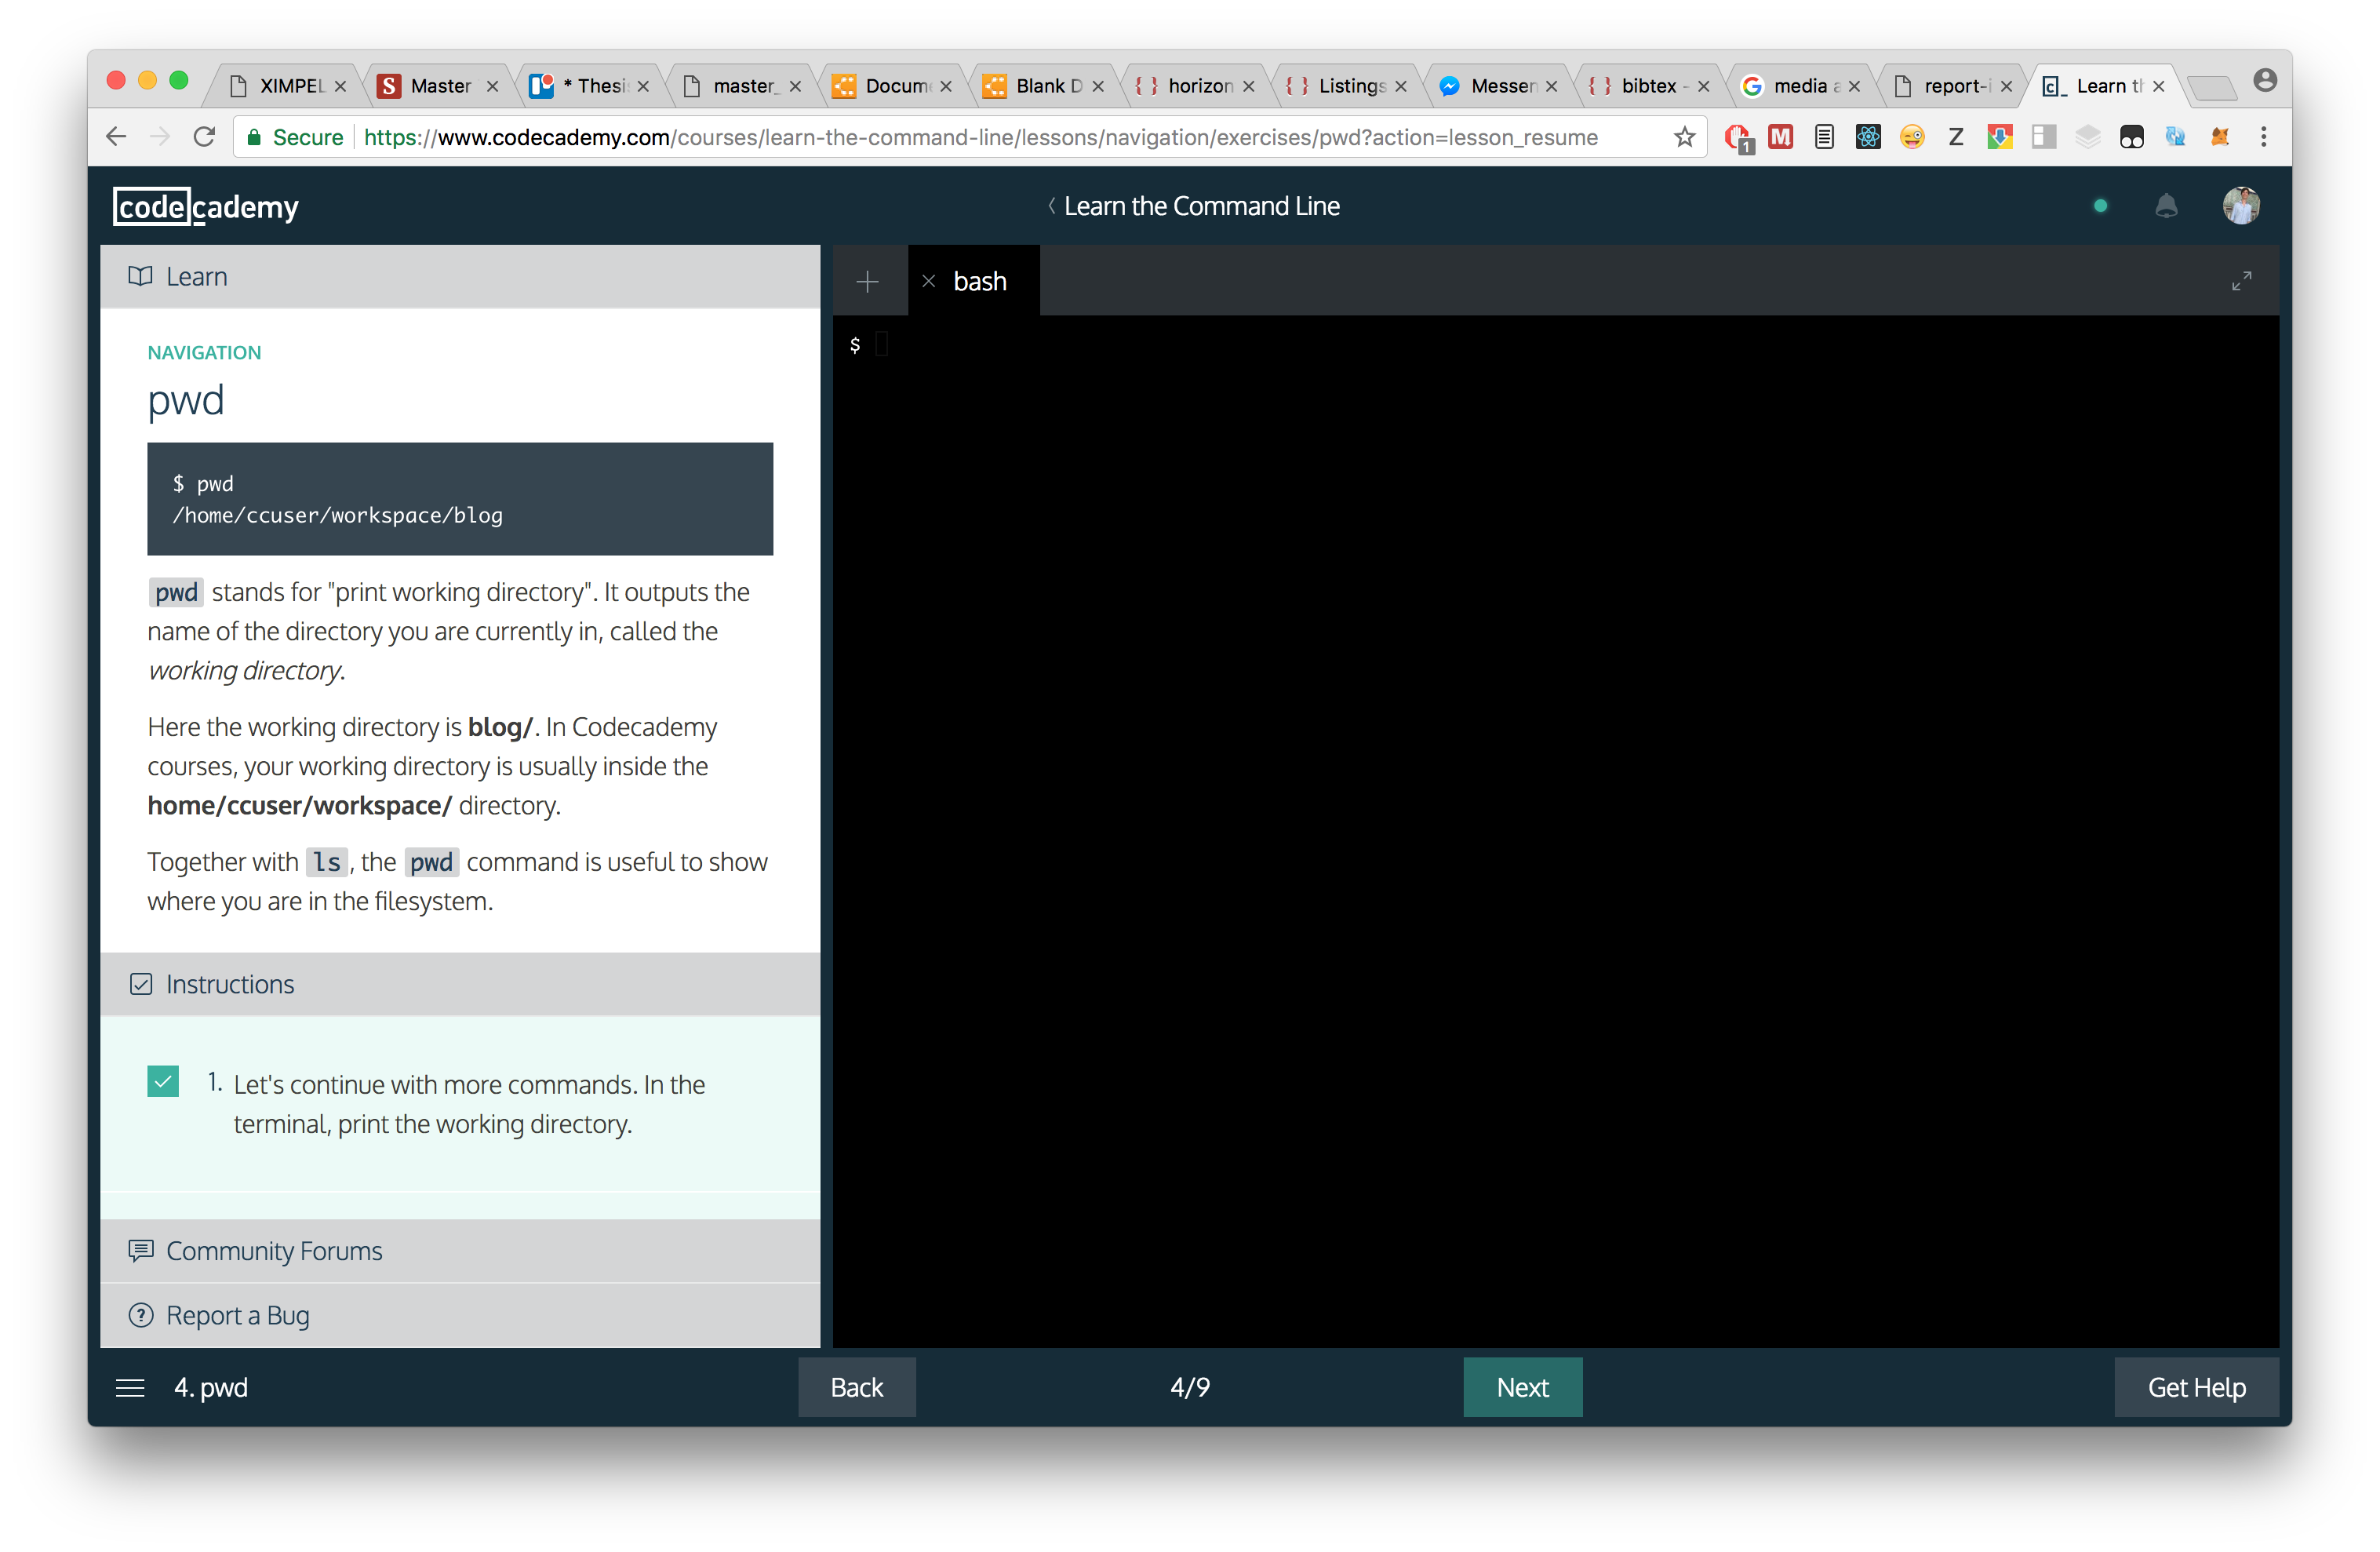
\includegraphics[width=1.35\textwidth, center]{codecademy_example.png} % quotation marks make sure file name does not display
    \caption{A lesson in the Codecademy command-line tutorial. This lesson shows how to use the print working directory command.}
    \label{fig:codecademy}
\end{figure}

When I first started recreating this command-line tutorial I realized two things. (1) It would be interesting to see how such a tutorial would be with video besides it instead of text and (2) I did not have time to recreate the whole tutorial so by using my artistic freedom I recreated the first two lessons which are about how to use the `pwd` and the `ls` command. By doing this the framework is going towards online education. Media itself is in most cases already a form of education, but by creating a command-line tutorial the XIMPEL framework moves more towards the interactive part of education. 

% \section{Requirements command-line tutorial}
The command-line tutorial requires two things. XIMPEL needs to be extended in order to play multiple media types. It could be possible to create a media type that plays video and has a terminal emulator which is too tightly coupled. This gave rise to exploration 2. The other requirement is that XIMPEL needs to be able to have a terminal of some sort. In this exploration I will focus on how I created a terminal application within XIMPEL.

\section{Architecture of the command-line media type}
In order to create a proof of concept I started looking and reverse engineering on how other command-line web applications were created. I took a look at: R-fiddle and CodeCademy. I also took a look at JSfiddle since I entertained the idea of executing JavaScript as a code tutorial. I quickly stopped entertaining that idea when I realized I had to use the `eval` function and would create a whole host of additional security hazards to XIMPEL. 

R-fiddle has the following architecture: it has a client, a server and it communicates via websockets (seen via Chrome Developer Tools). It spins up a virtualized container such as docker or vagrant in order to minimize security risks such as a shell with too much privileges on a file system that has sensitive information. By using virtualized containers for each new client, there is no file system with sensitive information and the shell does not have too many privileges \cite{r-fiddle}.

Codecademy sends an authentication token to a server along with other data via an xhr-request (in JavaScript parlance: they use AJAX) and send other relevant data with it in order to manage at what course the user is and if the user is logged in. The server answers back in JSON. Also Codecademy uses websockets to communicate with a terminal application (see figure \ref{fig:codecademy_websockets}). Presumably, they use some form of sandboxing.

The common architecture in common with both websites are: client, server, websockets as communication and presumably sandboxing. So the first step I created was creating a command-line tutorial in HTML/JS/CSS. Once that was completed I realized I needed to implement the client-side facing part of the terminal as a XIMPEL media type. Moreover, that media type needs to connect via websockets to a server. 

\begin{figure}
\centering
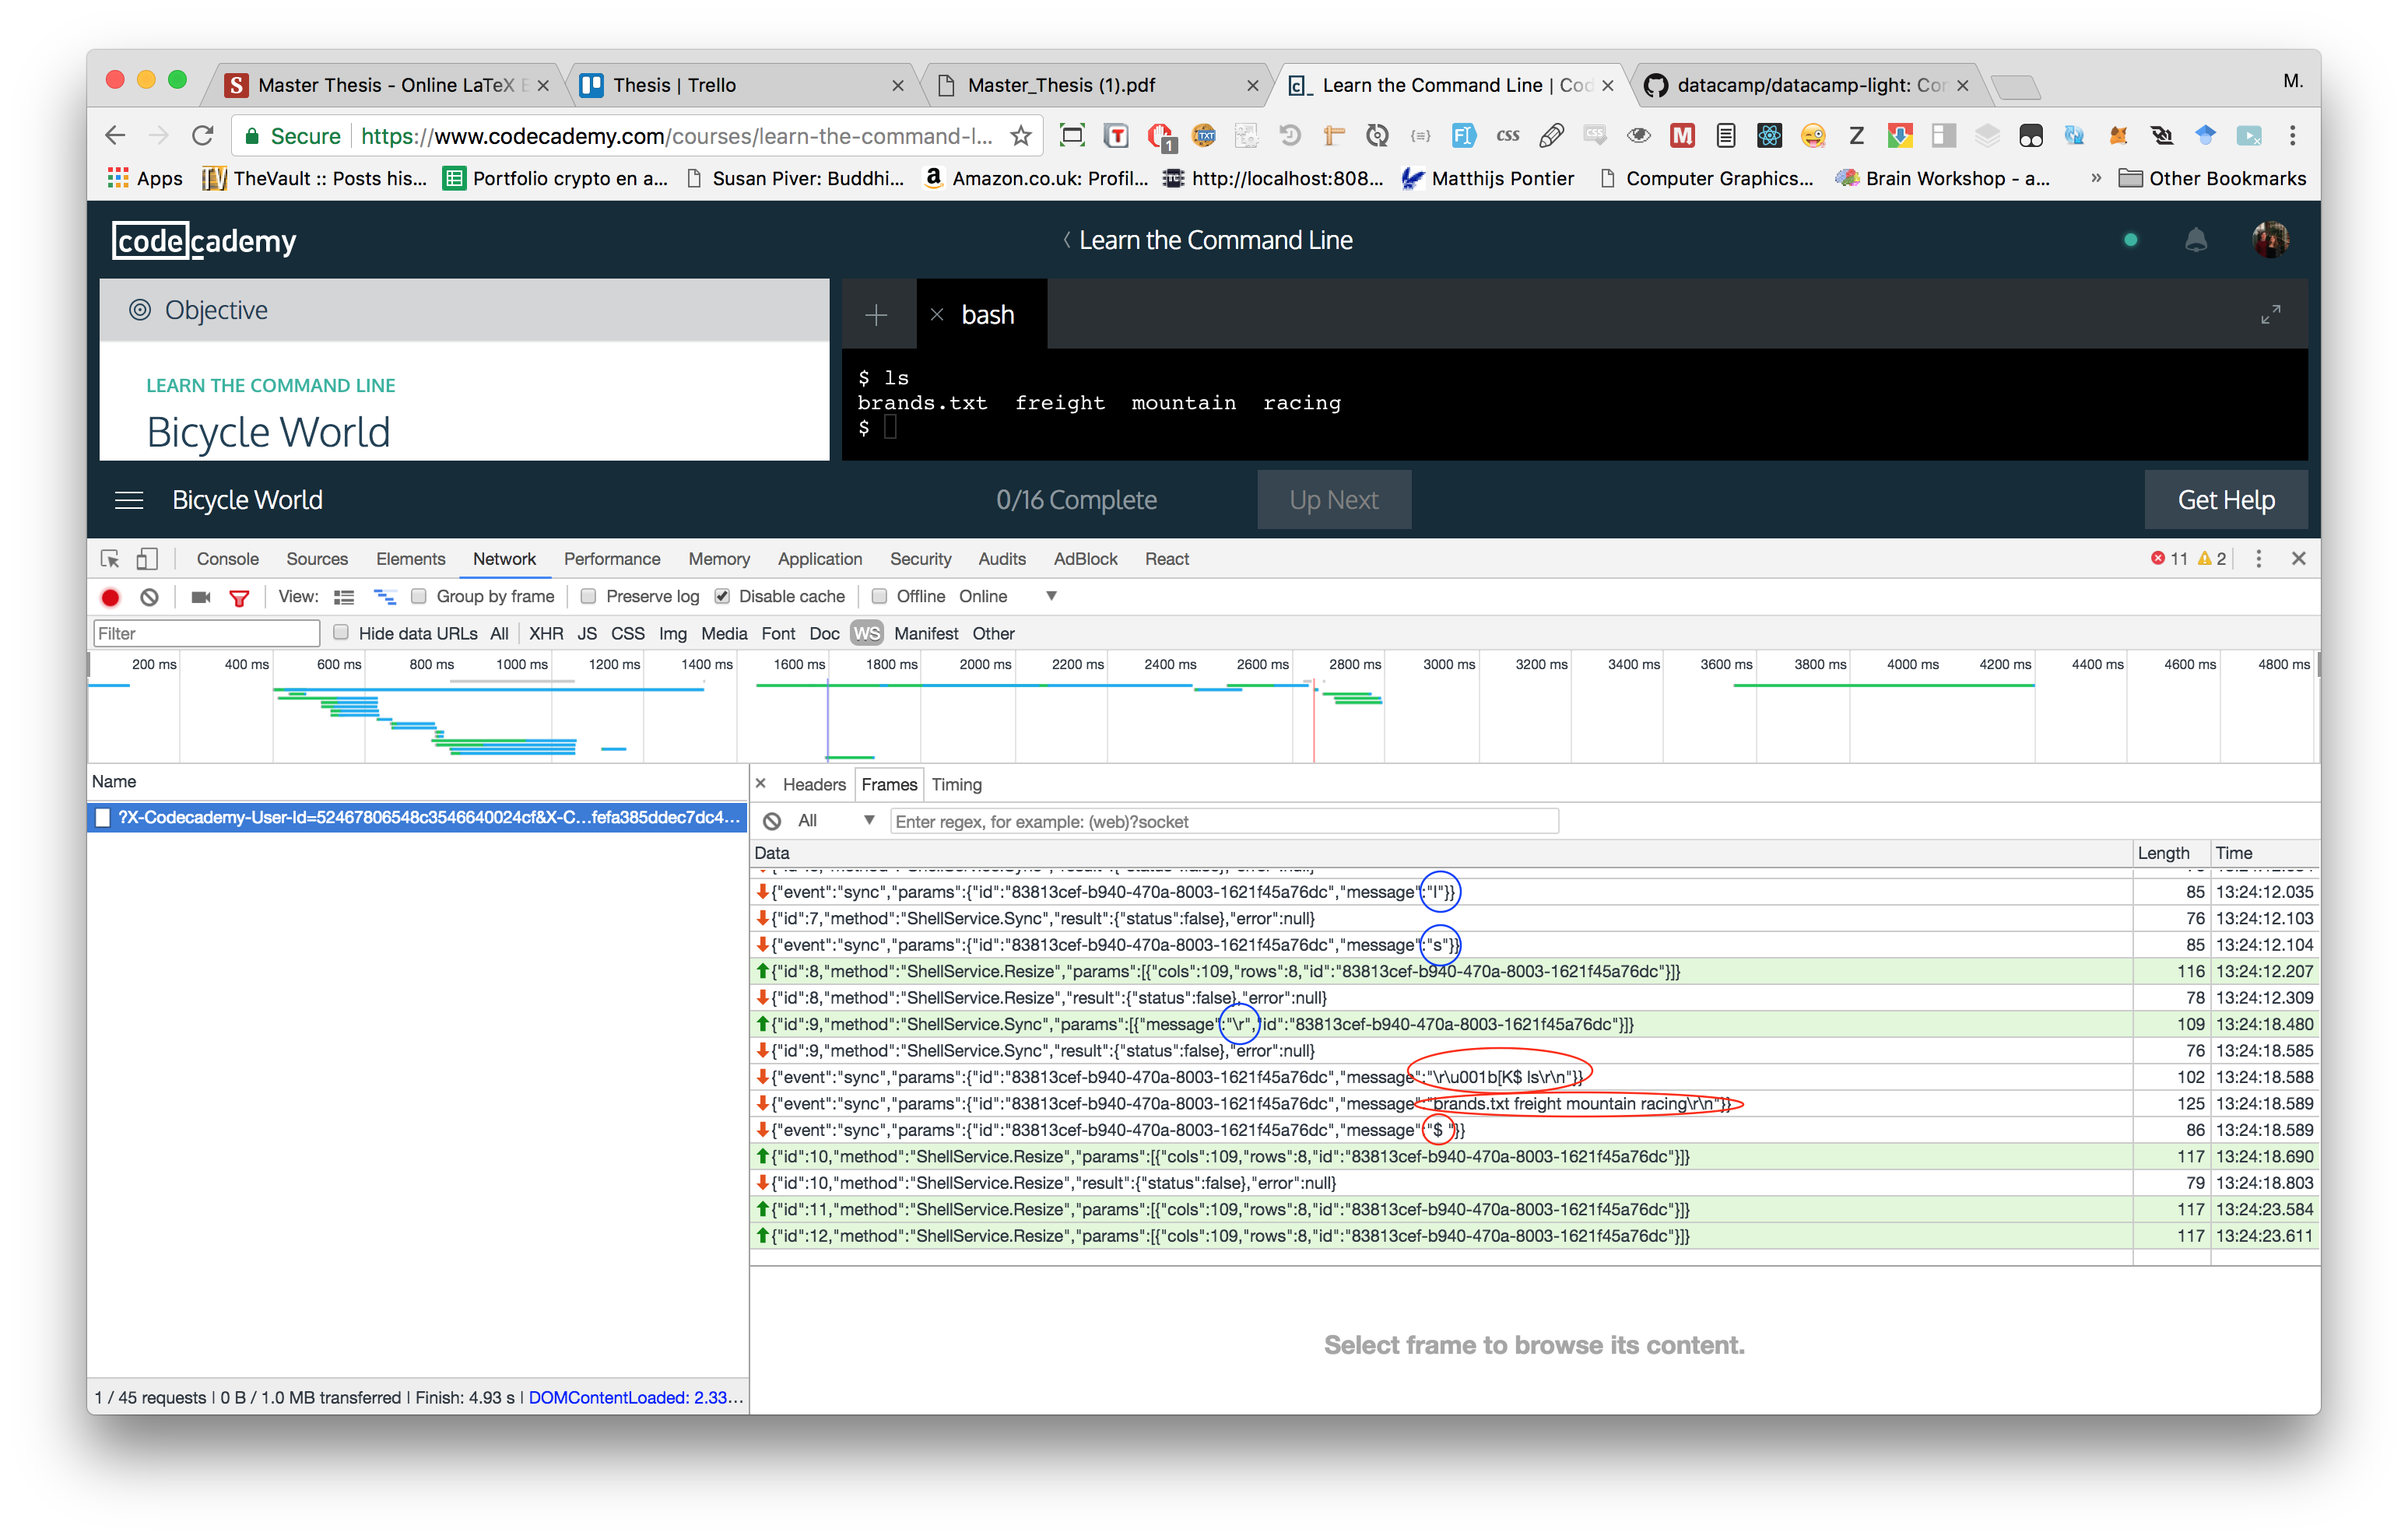
\includegraphics[width=1.35\textwidth, center]{codecademy_websockets.png} % quotation marks make sure file name does not display
\caption{Evidence that CodeCademy uses websockets to communicate with a terminal on some server. The blue circles shows data that is sent from the client to the server. The red circles shows data that is sent from the server to the client.}
\label{fig:codecademy_websockets}
\end{figure}

The current implementation has its server-side part implemented in NodeJS with the web server micro framework ExpressJS, which currently receives input data from the XIMPEL terminal media type via websockets. It furthermore spawns a bash shell and sends the data back to the terminal media type. Once it is there, the output of the bash shell will be displayed in the XIMPEL presentation. It has to be stated that this implementation is a proof of concept as it is not secure since the bash shell is not sandboxed with Vagrant or Docker, for example. Figure \ref{images:terminal_architecture} illustrates the client-server communication.

\begin{figure}
\centering
\includegraphics[width=1.35\textwidth, center]{images/terminal_architecture.png} % quotation marks make sure file name does not display
\caption{Communication example of the terminal media type. (1) The client sends a command, for example `ls`. (2) The NodeJS server sends this to a bash shell. (3) The bash shell sends a response to NodeJS, for example \textit{Desktop Documents} and (4) NodeJS sends that back to the client.}
\label{images:terminal_architecture}
\end{figure}

To conclude this section, creating a command-line tutorial has a couple of implications for XIMPEL. First, a lot of server-side web technology needs to be added such as NodeJS, ExpressJS and websockets. Furthermore, the devops tool Docker also needs to be understood. These web technologies are relatively new and not understood by all web developers and also not all web developers of XIMPEL which makes it harder to maintain XIMPEL. Second, it seems that XIMPEL is really suited for a micro service architecture. The reason for this is mostly because some media types require a server. To have a monolithic server for all possible media types in existence would harm the extensibility of XIMPEL, with microservices this danger is mitigated. Third, it is the question whether creating it as a media type is the way to go. XIMPEL also supports iframes, which means it could also have been implemented as an iframe for more control over the terminal. 

Finally to bring it back to education: XIMPEL its strength is in presenting non-linear paths, which could also be done for command-line tutorials. A serious student could perform its own manual dynamic difficulty adjustment by clicking the overlays which present possible harder or easier command-line challenges. The non-linearity of hypermedia is so built into the framework of XIMPEL that the idea is always a no brainer when one works with the framework. Yet, the idea of non-linearity is not seen in other popular online educational websites which means that hypermedia frameworks have an advantage in that aspect. 

\section{When is something hypermedia and when is it not?}
Hypermedia frameworks claim to be frameworks for rendering media items to the screen. While this is true, in the case of SMIL and XIMPEL they do much more. This is confusing, because two questions arise from this: (1) what is hypermedia? (2) Are SMIL or XIMPEL hypermedia framework or not? With regards to XIMPEL the answer is a clear no, since it is inspired by them but it is not one itself. SMIL 3.0 on the other hand is capable of interacting with parts of a web application and partially also created parts of a web application (see \cite{SMIL_lecture} around minute 25, it is a video). If all hypermedia frameworks are doing more than just enabling hypermedia content, then it needs to be established what hypermedia is and what it is not. Being able to make a distinction in that provides better vocabulary which aids categorical comparative analysis, much in the same way that the distinction between gender or sex provides categorical comparative analysis (e.g. females compared to males, two categories being compared). It may also shed light on the usefulness of non-hypermedia elements in hypermedia frameworks.

To begin answering the question: in order to answer when something is hypermedia and when something is not, it must first be asked what it means for something to be media on a computer. A literature search has been done, but unfortunately no relevant literature has been found. It is quite strange to not find literature on a very basic question such as: ``what is media?'' or its more slightly complicated version ``what is hypermedia?''

% Social media is defined as "(a) the information infrastructure and tools used to produce and distribute content that has individual value but reflects shared values; (b). the content that takes the digital form of personal messages, news, ideas, that becomes cultural products; and (c) the people, organizations, and industries that produce and consume both the tools and the content" (Howard & Parks, 2012, p. 359). Specific examples of social media sites include Facebook, Twitter and Instagram. The easy connective nature of social media sites greatly facilitates social networks, to the extent that they form a key part of this networked structure.  


The characterization of media falls into three distinct ideas, as I have seen so far: (1) mass media, (2) computer (multi)media and (3) social media. Common examples for each three is common knowledge for most people. For example, television, radio and the newspaper are seen as forms of mass media. Video, audio, images and text are seen as fundamental forms of computer media. Coincidentally the two have a very strong mapping with each other. For example, text and images appear in a newspaper. 

With social media the notion of what media is becomes more vague. Social media can be characterized as platforms where people are social on the internet. The usual suspects are: Facebook, Twitter and Instagram. But public internet forums, newsgroups or a guestbook could also be seen as social media. In all of these cases it is possible for people to communicate with each other through the use of computer (multi)media such as: video, audio, images and text (including emojis). 
Interactivity is new here and that is because with the two more old-fashioned forms of media, it always was a one way communication. 

Up until this point it could be argued that computation and manipulation of digital objects -- other than writing -- text do not need to be considered media. However, people call games media as well. And in games, everything is possible!

For our purposes, however, the characterization of media will not contain computation. A spreadsheet application is not a form of media and neither is a calculator. Other not media examples are: Finder, my text-editor, the command-line, a web browser, TeamViewer, Evernote, my FTP program, my mindmap editor, my colormeter, my screencast recording software, my vector graphics manipulation tool, Unity3D, Java, Preview, a Git viewer, Activity Monitor, my time tracker and paintbrush. This is more than eighty percent of my visible applications in my Mac OSX dock. Two applications could be considered social media, which are Colloquy (an IRC client) and Slack. However, since the information is not public (like guestbooks and forums) they may also not been seen as social media.

Finally, what all forms of media have in common is that they use the senses. For example, one hears twigs cracking slightly, above the soft noise of a fuzzing wind; furry hairs and two humongous toes are seen in the corner of an eye; a huge arm grabs your puny wrist in comparison and in a shock you realize: ``It is Bigfoot!\footnote{As much as I love furry huggable creatures I do not believe in most of them other than teddy bears for sale at the toy store.}'' If this would be a real experience, then it would not be (multi)media. However, if this experience is fabricated through: screens, paper and other various forms of technology then it is (multi)media. The multimedia researcher Anton Eli\"ens agrees with this idea. He says that multimedia is everything that uses (sensoric) media experiences such as vision and sound \cite{eliens2017:private}.

% Should I characterize media? -- leave it up to the reviewers

So what is hypermedia? Every form of media that uses vision and sound and does not contain a form of computation other than the computations that are relevant for displaying the media itself. Furthermore, hypermedia is linkable, just like hypertext. 

This means that by creating a command-line tutorial in XIMPEL, the framework has expanded beyond hypermedia. It already has been expanded beyond hypermedia in recent editions by having iframe support, so the idea that XIMPEL is only an hypermedia framework is not the case anymore.

XIMPEL is, however, mostly a hypermedia framework in its philosophy, since no programming knowledge is needed in order to create hypermedia presentations. For advanced XIMPEL users, it is more than only hypermedia. It is possibly anything that a web application could be. But XIMPEL does treat its extensions as media, even if it is an application like a command-line. This means that every extension (application or media) is able to: play, pause, stop and resume. Since it is arguable that XIMPEL is not a hypermedia framework the play, pause, stop and resume feature has less of a justification as well.

%Eliens noemt het interactive video
The conclusion for this part of the exploration is an unusual one. It is strange to wrap web applications like a terminal into custom media types. It does not seem useful to add multimedia features to this (i.e. play, stop and pause functionality). While it is possible and it works relatively well, the play, pause and stop functionality seems redundant. From a development point of view, it needs to be considered to what extent stop, play and resume functionalities should be obligatory for media types. On the other hand, a fairly easy solution is to leave an empty function body for the resume functionality. In exploration 6, I show how to program media types for mitigation of immediately stopping playback after a subject switch. So the resume and stop functionalities can be completely mitigated.

% I have to think about this conclusion

A second conclusion is that the power of XIMPEL is its playlist. For example, just by typing `<terminal>` one is able to create a complete terminal experience! This idea sparked exploration 3: recreating XIMPEL with ReactJS of which the rationale will be discussed in its relevant chapter (chapter \ref{chap:exploration3}). One of the ideas in ReactJS is similar compared to the XIMPEL playlist, which is: everything is a component. Everything in the XIMPEL playlist is a component as well.

% To do: see if you can implement this
% My final opinion on the latter question is: no not per se. XIMPEL borrows ideas from hypermedia to make sure that creating educational immersive gameplay (with media) happens a lot quicker. However, the moment XIMPEL needs to be adapted to MOOCs, the idea of XIMPEL being only a hypermedia framework should be abandoned.


% Closing paragraph
In closing, the distinction of when something is hypermedia or not justifies and delineates the relevance of hypermedia frameworks. Hypermedia frameworks keep themselves relevant by having extensibility with application components or interactibility with application parts of any platform it resides on. Furthermore, hypermedia frameworks with extensibility in mind seem not to trade any performance penalty compared to pure hypermedia frameworks, other than losing development and design focus on hypermedia features. However, a more not well-known trade-off is that by doing this a hypermedia framework becomes more complex and one could study whether it is not pedagogical to keep hypermedia frameworks simplistic, or fork hypermedia frameworks to keep the forked version simplistic. In this section it has been found that sticking too much to the hypermedia ideal harms extensibility and promotes a pure hypermedia approach. An unexpected conclusion is that the power of XIMPEL is in its playlist. Hence exploring this question led to the exploration of a software engineering question described in chapter \ref{chap:exploration3}.

\subsection{Conclusion}
How would XIMPEL need to be extended in order to create a command-line tutorial? A server-side architecture needed to be researched, implemented and a parallel player needed to be created (see chapter \ref{chap:exploration2}). This changes XIMPEL from being a front-end framework built with hypermedia philosophy to being a full-stack framework built with a hypermedia philosophy. One other way is to implement a terminal media type and not changing the nature of XIMPEL from being front-end only to full-stack would be by simulating the x86 architecture via JavaScript. This has been done before but for the constraints of the exploration described in this chapter it would take too much time.

What are the implications of mixing a hypermedia application with another application? It leads to the realization that a pure hypermedia approach has more disadvantages than advantages. This furthermore means that research should be done into the interplay of hypermedia and non-hypermedia elements in a hypermedia framework. Many hypermedia or hypermedia-like frameworks are use-case driven. An exhaustive literature review of comparing hypermedia frameworks and its use cases will shed light on a possible more abstract or generic classification of topics for which hypermedia frameworks are useful for.
% \chapter{Exploration 2: extending XIMPEL for playing media types concurrently}
\label{chap:exploration2}
%no conlclusion in his thesis on how HTML 5 influences hypermedia
I read Stefan Bruins his thesis over and over. While a thesis is academic, I detected a form of sadness in it, a regret perhaps. There was a longing to play media items in parallel. Everything was set for it: the architecture expected it, in Stefan his thesis it was written about and because of the command-line tutorial, I needed it. However, it was not there.

At the time I did not think much of it, but at the end of my thesis I realized that parallel media playback and parallel media items interfacing with applications is a topic of research for computer scientists that could provide new insights into the nature of computation and human-computer interaction. Moreover, parallel media playback from a hypermedia standpoint is inevitably linked with multiple time lines. Because of this it has some resemblance to time travel. It is even possible to have a poor man's simulation of time travel with parallel media playback! But let's visit this topic in the future.

% Note to self: Stefan geeft geen justification voor parallel media playback, daarnaast geeft het twee tips
% Doe het via de media player
% Doe geen nested parallel tags
% Ook hier geeft hij geen justification voor
Let's start from the beginning: Bruins explored in his thesis whether XIMPEL could be ported to the web without the use of plugins like it was programmed in the past (with the Flex SDK, As3 and Flash). In other words could it be ported to the web with: HTML5, CSS and JavaScript? The answer was a resounding yes \cite{stefan2016}. Bruins also suggested future work to be done on the XIMPEL platform. One of the most prominent examples is the creation of a parallel media player. XIMPEL has been architected with a parallel media player in mind. Therefore, programming a parallel media player will give an even more conclusive answer to his research question of how one can be programmed. Furthermore, implementing a parallel media player will allow us to have a closer look at possible technical difficulties regarding HTML5 and attempting to play multiple videos in sync. 

On another note, creating a parallel media player gives much more insight as to what hypermedia is. Simply creating a framework that plays one media element at the time is a rather limited experience in the form of hypermedia. Creating a parallel media player for XIMPEL would mean that more video and audio and custom media types could be played (note: it was already possible to display multiple images and text via the overlay mechanism and there was iframe support). Parallel media playback is possible in SMIL since version 1.0. However, SMIL and other hypermedia frameworks does not seem to offer a plugin like extensibility which means that the implications of parallel media playback and application media types (e.g. `<terminal>`) are left unexplored. %no ref -- too much work


\section{Architecture of parallel playback}

By looking at the architecture of XIMPEL and how the sequence player was implemented, implementing a prototype of the parallel player has been more doable than without it. However, there were a couple of caveats in the original architecture of XIMPEL as stated in Bruins thesis (see figure \ref{fig:original_architecture}). First of all, the figure suggests that a `SequencePlayer` is able to play another `SequencePlayer`. After testing the following playlist (see playlist \ref{playlist:sequenceplayers_wrong}) this is demonstrably false. Fortunately, it is false because there is no need for a `SequencePlayer` playing yet another `SequencePlayer` that will then play media types in sequence. The reason is: one `SequencePlayer` already plays media types in sequence!

\begin{lstlisting}[language=XML, caption=This playlist contains a nested sequence tag and therefore does not work. This demonstrates that the architecture in figure \ref{fig:original_architecture} as outlined in Stefan Bruins\cite{stefan2016} his thesis (fortunately) does not work as prescribed., label=playlist:sequenceplayers_wrong]
<ximpel>
<config>
    <enableControls>true</enableControls>
    <controlsDisplayMethod>overlay</controlsDisplayMethod>
</config>
<playlist>
    <subject id="lesson1">
        <sequence>
            <sequence>
                <message text="hey" />
            </sequence>
        </sequence>
    </subject>
</playlist>
</ximpel>
\end{lstlisting}

\begin{lstlisting}[language=XML, caption=this playlist does work and serves as a counter example to playlist \ref{playlist:sequenceplayers_wrong} which has a nested sequence tag., label=playlist:sequenceplayers_right]
<ximpel> 
<config>
    <enableControls>true</enableControls>
    <controlsDisplayMethod>overlay</controlsDisplayMethod>
</config>
<playlist>
    <subject id="lesson1">
        <sequence>
            <message text="hey" />
        </sequence>
    </subject>
</playlist>
</ximpel>
\end{lstlisting}

The current architecture has been updated to reflect the implemented changes as well as the intention of XIMPEL (see figure \ref{fig:architecture}). In its current architecture the XIMPEL player always calls \textit{the} `SequencePlayer`. And a `SequencePlayer` can either call a `ParallelPlayer` or a `MediaPlayer`. A `MediaPlayer` plays a `MediaType` (e.g. video or audio). A `ParallelPlayer` plays multiple `SequencePlayer`s. By doing it this way it is possible to allow nesting of parallel tags. In some cases nested parallel tags is desirable since at every level of the multimedia presentation an author will able to decide which parts of the presentation have to play in parallel and which parts of the presentation have to play in sequence.

These players have corresponding models. So a `SequencePlayer` plays a `SequenceModel`, a `ParallelPlayer` plays a `ParallelModel` and a `MediaPlayer` plays a `MediaModel`. From `MediaModel`s, `MediaType`s are constructed.

The extensibility of XIMPEL and playing media types in parallel allows for one unexpected idea: one can extend XIMPEL with applications that are not multimedia. This question has been explored in another part of this thesis (see chapter \ref{chap:exploration1}).

\begin{figure}
\centering
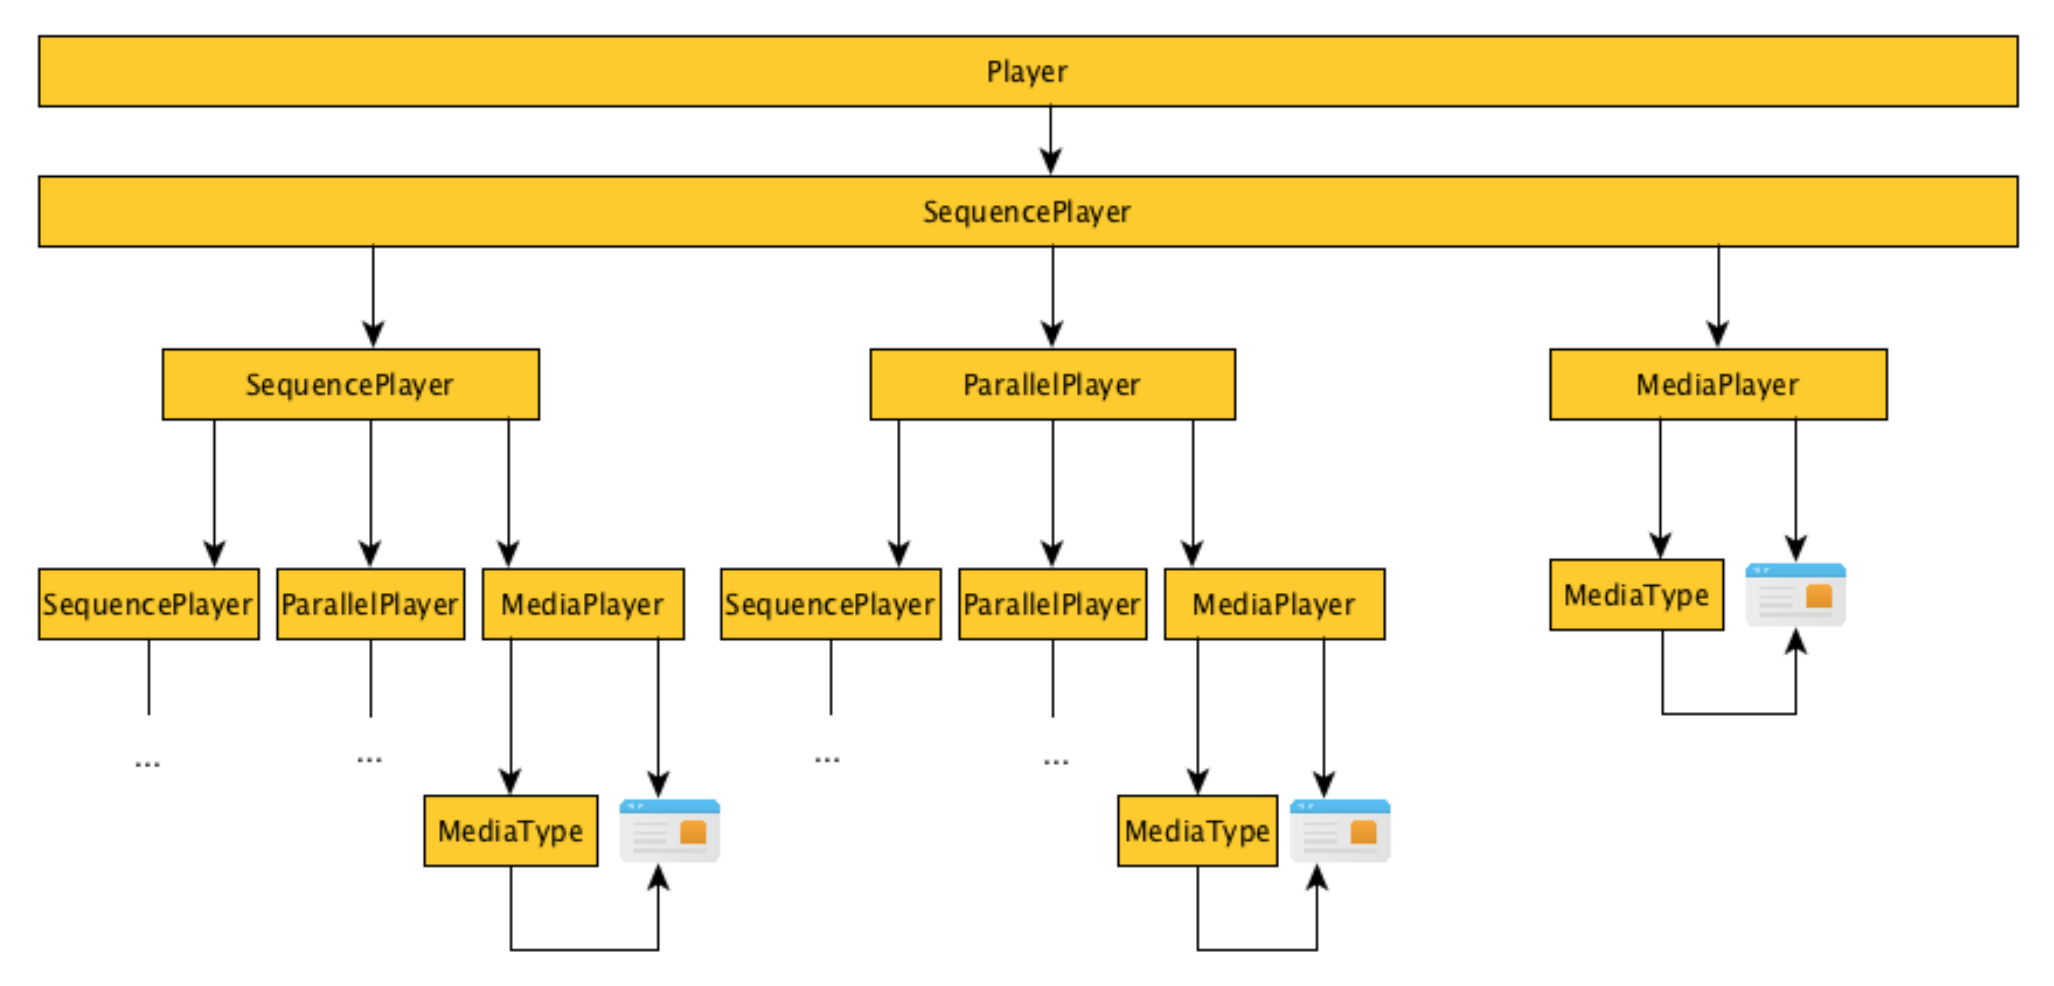
\includegraphics[width=1.35\textwidth, center]{ximpel_original_player_architecture.png} % quotation marks make sure file name does not display
\caption{The original player architecture of XIMPEL. The media type gives rise to media which can be: video, audio, image, text or a custom defined media type. This architecture has been proposed and (partially) implemented by Stefan Bruins \cite{stefan2016}. It has been demonstrated by me that nested SequencePlayers have not been implemented and I also explained why this does not need to happen in the beginning of this chapter. The diagram shows the possible valid children a player would be able to play.}
\label{fig:original_architecture}
\end{figure}

\subsection{Implementation of parallel playback}
For the architecture of any player in XIMPEL (e.g. a parallel, sequence or media player) there is a pipe line. (1) It starts with parsing the XIMPEL playlist, which is in XML. (2) The data parsed by the XML syntax get put into an in-memory configuration object, which holds the details of the XIMPEL playlist. (3) The player itself uses, in most cases, a subset of the in-memory configuration object\footnote{Since the whole object is the complete playlist, so a part of the in-memory memory object it is the relevant part of the playlist that needs to be played}. Each individual part of the pipe line is explained in its own section.

\subsubsection{The parallel player and parsing}
The first part of implementation that needed to be programmed was the parser. The parallel player needed to be registered as a valid child, since it otherwise would refuse to parse the `<parallel>` tag. In the `processSubjectNode` method the `processParallelNode` method is called which will return a parallel model which is part of the in-memory configuration object. The method will determine the info of the `<parallel>` tag (e.g. its parent and children) which is needed to loop through its children. While looping through its children, the method will determine whether this particular `<parallel>` tag has: `<sequence>` tags, `<media>` tags or custom defined media type tags. It will then add those to the parallel model.

\subsubsection{The in-memory configuration of the parallel player}
The `ParallelPlayer` uses a `ParallelModel`. The `ParallelModel` itself is nothing more but a glorified array, as of now. It has a property called `list`. It also has a method called `add`, which means: add the children of the `<parallel>` tag to this list. These children are wrapped in a `SequenceModel` since it is one `SequencePlayer`, managing one media item. It furthermore inherits the `get` and `set` method from `ximpel.Model`. The methods and variables in every method are completely identical to the `SequenceModel`. It only differs from the `SequenceModel` with the idea that the playing order of the `ParallelModel` is to play everything at once, instead of in a default or random sequential order. 

\subsubsection{The parallel player itself}
The major code revisions were regarding the `SequencePlayer` and creating the `ParallelPlayer` itself. XIMPEL always has a top `SequencePlayer` (i.e. \textit{the} `SequencePlayer`), it needs to be aware of how to start a `ParallelPlayer`. For example, when the `SequencePlayer` needs to stop it also needs to stop the `MediaPlayer` and the `ParallelPlayer`. Another example is that there needs to be a method in the `SequencePlayer` to play a `ParallelModel`. All the method really does is passing it on to the actual `ParallelPlayer`, but the `SequencePlayer` still needs to know about it.

%Should I apply variable modifiers?

The implementation of the `ParallelPlayer` itself is inspired by the `SequencePlayer`. Unlike the `SequencePlayer` which plays media types in sequence, the idea is to play everything all at once. The architecture of XIMPEL already allows for players to start playback for other players. In the architecture outlined in figure \ref{fig:architecture}}, a `ParallelPlayer` will have multiple players as its children of some kind. 

As possible candidaties, one could consider the `ParallelPlayer` to have multiple `MediaPlayer`s, or multiple `SequencePlayer`s, or a custom implementation of multiple players. For sake of simplicity I chose that the `ParallelPlayer` is able to have multiple `SequencePlayer`s, simply for the reason that a `SequencePlayer` is a wrapper for a `MediaPlayer`. Because it is a wrapper, it has the same and extended functionality. This extended functionality was eventually needed when I realized later on that you might want to have a sequence while you are playing something parallel. This is entirely possible with multiple `SequencePlayer`s, but it would be more tricky to create with multiple `MediaPlayer`s.

For all the other functionalities the core idea of the `ParallelPlayer` is that all `SequencePlayer`s need to be: played, stopped, paused or resumed. In other words: everything a normal `SequencePlayer` does, a `ParallelPlayer` does too but then for multiple `SequencePlayer`s. The diagram below shows the new architecture of XIMPEL on a high level including the newly implemented `ParallelPlayer` (see figure \ref{fig:architecture}).

\section{Conclusion}
A conclusion on such a technical subject as this is fairly straightforward: parallel media playback works and no issues have been observed as of yet. Other designs were possible but they have not been investigated. On another note, the creation of the parallel player allows for parallel playback, which allows the terminal media type of exploration 1 to be used in a much more useful manner since it is now possible to add video playback with it. Parallel playback allows for multiple media items of the same or different media types to complement each other through the ways such media items present their information.

However, such a conclusion is too short to be satisfying. Moreover, since this thesis is an explorative one it may be fruitful to know how far we have come. So in the remainder of the conclusion we are going to take a step back.

% what is the relationship between XIMPEL and education? And how does XIMPEL need to be improved for it to better serve education? 
Since exploration 1, I started with the question of how XIMPEL and education relate and how it needs to be improved, I now stumbled upon a new question. What are the implications of parallel media playback? It is mostly the latter question that will be answered in the remainder of these pages. This is not because I wanted to answer it, it is because I stumbled upon many questions and issues going forward with parallel media playback. 

Let us look in the future regardless. The `ParallelPlayer` has a lot of implications such as the user need for a media item surviving a subject switch (MISSS) when a user jumps to a new subject (see exploration 6) or the implications for time scrubbing are so numerous that it poses serious design issues (see exploration 5). The biggest implication of all is that everything is a lot less complicated when the developer only has one playing media item at a time to worry about instead of as many as a `ParallelPlayer` allows. Currently, XIMPEL is now able to play playlist \ref{playlist:example_playlist}, which is in appendix \ref{chap:exploration2_appendix}, which means it is able to play parallel media.
% Note that the media and sequence tags can be interchangeably used. 

Let us look to the next exploration. Exploration 1 sparked exploration 3. So for the next exploration, ideas about parallel media playback will be left alone. These ideas come back in exploration 5 and 6. So dear reader, I now give you a choice. Explorative reading is an art in itself as well.

\textbf{Option A:} You can either start reading exploration 5 and 6 if you want to know more about parallel media playback.

\textbf{Option B:} Or, you can start reading exploration 3 and read how I recreate the majority of XIMPEL to ReactJS.

The choice itself centers around the following question: do you want to thematically read all the themes in such a way that it is easier to digest? Choose option A. Do you want to read how the thesis happened in chronological order? Choose option B. Regarding option A, it is my suggestion to read the thesis in the order of: exploration 5, exploration 6, exploration 4 and exploration 3. Exploration 3 and 4 could be swapped since it is exploration 1, 2, 5 and 6 that are thematically linked. Regarding option B, I would like to remind the reader that the correct chronological order of how the explorations have been done are: exploration 3 (read only until the first subsection), exploration 4 to 6 and back to the rest of exploration 3. 

% Maybe in exploration 1?
% Another implication pertaining to parallel playback and one that has been shown in exploration 1 is that it allows a XIMPEL author to play multiple media items on one page. One use case for that is education, which benefits from playing multiple media items regarding course creation. The odd fact has been observed that some media items are not items of media but rather applications disguised as media items. This seems strange, but it works. The strangeness might be because the philosophy of hypermedia in general has been formulated when the view of the web as a hypertext document was still in vogue. In 2018, the idea of a website as an application is a lot more trending\cite{garrett2000, paulson2005}. 

% Jesse James Garrett wrote in 2000 about it and stated:``The Web was originally conceived as a hypertextual information space; but the development of increasingly sophisticated front- and back-end technologies has fostered its use as a remote software interface. This dual nature has led to much confusion, as user experience practitioners have attempted to adapt their terminology to cases beyond the scope of its original application.\cite{garrett2000}'' He saw a clear difference between the web as software interface and the web as hypertext system. Five years later an industry trends article appeared titled \textit{Building Rich Web Applications with Ajax} in the peer-reviewed IEEE Computer Society in which they shed more light on this trend, through the help of Garrett his visual image\cite{paulson2005}.

% One could ask: since the philosophy of the web shifted, how should the philosophy of XIMPEL react to it? Should it stay the same? Or should it adapt? The concepts of hypermedia have not been updated with this paradigm shift about the web. If the philosophy of hypermedia adapts, then it may be possible to reconcile the whole media versus non-media paradox regarding the extensibility of XIMPEL. While this question is not an implication of parallel media playback, the process of creating the parallel media player did trigger it.


\begin{figure}
\centering
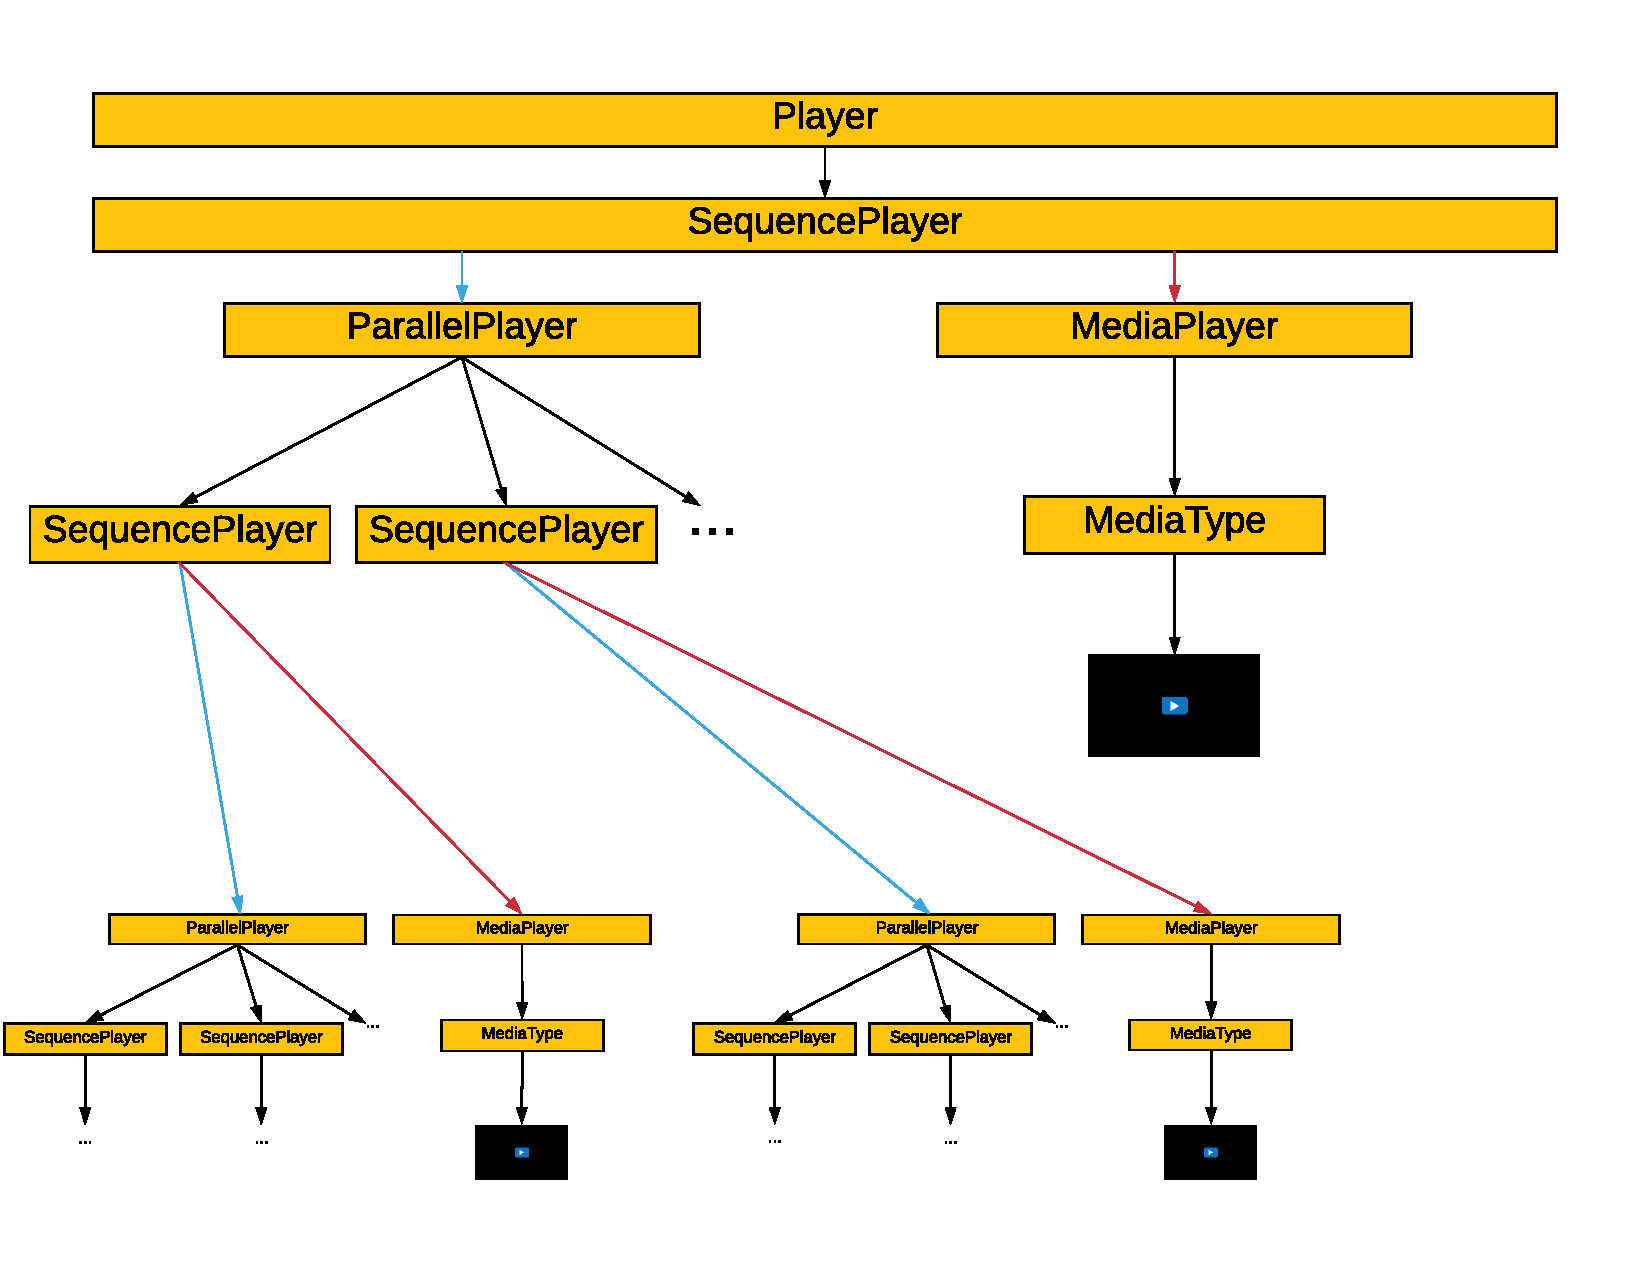
\includegraphics[width=1.35\textwidth, center]{ximpel_player_architecture.pdf} % quotation marks make sure file name does not display
\caption{The current player architecture of XIMPEL. The media type gives rise to media which can be: video, audio, image, text or a custom defined media type. The diagram shows which possible players can be played but also how many players another player can play. A blue or red line indicate that the player of which the line originates needs to choose between one of them. A black line means that a player will be invoked by another player.}
\label{fig:architecture}
\end{figure}



% 
\chapter{Exploration 3 (part 3): assessing the benefits for porting XIMPEL to React}
\label{chap:exploration3}

% Leg de titel uit en waarom part 1 en 2 weg zijn
Why would a chapter start with part 3? There is of course only one sensible explanation: part 1 and part 2 -- also described as first attempt and second attempt -- have been kidnapped. On a more serious note, the relevant elements of part 1 and part 2 are in this chapter as well, but it is part 3 that presents how XIMPEL could be effectively and efficiently be ported to React. However, in an attempt to preserve how the exploration went, this chapter has been labeled part 3 and the other two parts are in the appendix.

% Leg uit waarom je voor ReactJS koos
With that said, ReactJS is hip, new and shiny. It introduces a relatively unknown paradigm to web developers called reactive programming. I wanted to work in this language because the web community seems to settle on this as a best practice method of creating web applications. Moreover, if my thesis supervisor can demand that I work on his framework pure for promotional reasons, then I can decide I learn a new framework for self promotional reasons. Later on I also justified the use of React academically but I do not want to shy away from the inherent selfishness that academia has. If science is a form of truth discovery, then the truth of its process should not be hidden.

Related to this is that I wanted to create the same type of exploration that Stefan Bruins did. If Stefan Bruins can port XIMPEL to JavaScript and call it academic, then I can do the same for porting the JavaScript version of XIMPEL to React. I believe in both cases the research question of ``is it possible?'' could be answered a priori with a ``yes.'' However, like Stefan I am an empiricist and the strongest form of evidence is through physical demonstration. Moreover, I altered the research focus to whether XIMPEL written in ReactJS (from now on called XIMPEL React) has more advantages than XIMPEL written in JavaScript + jQuery (from now on called XIMPEL JS). That answer is a lot tougher to answer a priori and hence an actual implementation, including a write up of the whole implementation experience is needed.

% I should tell here that XIMPEL has one powerful feature that React has as well: the ability to create components.
On another note, this started out as exploration 3, but part 3 of the exploration occurred later than exploration 4, 5 and 6. Therefore, it could also been seen as the final exploration. 

The reason this exploration started in the first place is because XIMPEL shares an idea that ReactJS has as well. They both have components. XIMPEL has it in the form of a playlist, where every component could be seen as a sort of invocation towards execution of the actual component. It is analogous to a function invocation and function definition. ReactJS is not bounded by a playlist, it has components everywhere; it also has the idea of component invocation and component definition, like XIMPEL. Figure \ref{images:architecture_playlist_to_component_mapping} shows this thought.

My questions specifically regarding this exploration are: is it possible to make use React and its ecosystem to port XIMPEL to React efficiently and effectively? Moreover, what are other possible benefits or disadvantages regarding this port? 


% glossary:
% media type: a specific media class name (e.g. Video or Audio) in both plain JS XIMPEL and XIMPEL React
% media item: a specific instance of any media type

% TO DO
% Short story exploration 3
% Discussie opnemen over welke features erin en welke niet -- justification
% Op welke manier passen questions in XIMPEL?
% React als ecosysteem? Te doen?
% Maintainability
% Is de React codebase zinvol? Voor? Tegen? Eventuele uitbreidingen?
% Duidelijk formaat exploratie. (geldt voor alle exploraties)
For porting XIMPEL to ReactJS I thought it had the following advantages:
\begin{itemize}
    \item A lot of parsing logic could be done via ReactJS and Webpack by transforming the XIMPEL playlist to a declarative language that is completely compliant with JSX. So there is no need to create a parser.
    \item The virtual DOM would replace the in-memory configuration code that has been written for XIMPEL. So there is no need to write in-memory configuration code.
    \item Cross-browser support is suddenly managed by the maintainers of the ReactJS framework.
    \item By teaching XIMPEL to students, it is needed to teach about ReactJS to students who want to extend XIMPEL. This introduces them to some of computer science concepts implicitly.
\end{itemize}

% Veel parsing logic kan via React worden gedaan en hoeft niet meer worden opgeschreven, omdat de XIMPEL playlist basically een JSX datatype wordt.
% Hetzelfde geldt voor de playlist tree dat in het geheugen wordt opgeslagen: React doet dit via de virtual DOM.
% Het maken van mediatypes en dergelijke wordt ook een stuk flexibeler, omdat het aanmaken van een mediatype betekent dat er een extra React component wordt gemaakt.
% Nu kun je mensen stiekem HTML/CSS onderwijzen als ze een XIMPEL playlist maken, terwijl de kern van XIMPEL blijft bestaan. 

% Een mogelijk nadeel:
% Een nadeel is dat elke child node (HTML of React Component) onder elke child node mag waardoor er invalid playlists kunnen bestaan. React is misschien te expressief. Het nadeel is volgens mij niet heel groot, omdat de gebruiker er visueel mee wordt geconfronteerd.

In short, the idea was to see if it is possible to make the ReactJS framework work for us. If this is possible, then we as XIMPEL developers have a free lunch! Who does not want a free lunch?


% De voordelen 1 tot en met 3 blijken onwaar te zijn. Ik kwam erachter dat veel parsing logic en playlist tree logic nog steeds geprogrammeerd zou moeten worden, en het maken van eigen mediatypes zou net zo flexibel zijn -- niet flexibeler. Voordeel 4 is echter wel waar, mits je XML opgeeft en studenten laat programmeren in JSX, maar dan wordt XIMPEL ook wat complexer helaas. Mijn XIMPEL React programma laat wel zien hoe je XML kan vertalen naar React components, wat ik supergaaf vind om te zien! :)

To validate these assumptions I made a very simple prototype of creating a custom React component in an XML file. The XML file would be read in by a React class that I programmed. What I found is that this exploration failed so dramatically that for more than 6 months I believed to have invalidated most advantages. You can read a full write up of the failure in appendix \ref{chap:exploration3_appendix_part1}.

However, by writing the chapter 6 months later, I was forced to take a closer look at the source code. Because I needed to look at the source code, I needed to look at the dependencies. And when I looked at the dependencies, I noticed that the XML parser of Webpack uses a library in order to parse the XML. There seemed to be a small detail that I missed. Upon further inspection this dependency of the XML parser of Webpack showed that the XML parser was configurable! Unfortunately, I did not see this before. So I could do a lot more in my second attempt, which is described in the next section.

\section{Webpack XML parser setup}
There were two modifications that allowed for a much more successful exploration compared to the first time. First, I modified the parser to have an explicit tree structure by preserving order between siblings and parent-child relationships. In general, it is the question whether an XML document needs this type of order preserved since some XML documents could be treated as an unordered set. 

For XIMPEL, it is needed that the XML document would be parsed as an ordered array. This feature gives more power to the programmer, in the same sense that a Turing complete system has more computational power than a finite state machine. Without order there is chaos, and in this particular case there would sometimes be no way to determine which media item (such as a video or image) or subject should be loaded first.

The second modification helped a lot in code readability. While it is not as game changing or groundbreaking as the first, code readability is a necessary requirement for a fruitful collaboration on any software project. For example, the default setting to denote attributes of a parsed XML tag itself was `$`. To denote inner text it was `_`. And children was `$$`. I renamed this to: `attributes`, `text` and `children` respectively.

%TO DO: some bug is in here!
\section{Implementation methodology of the second and third attempt}
In the second attempt of this exploration I tried to explore if I could re-implement XIMPEL quickly since the possibility of it is one of the main questions. I did not consider architecture -- or even best practices for programming React. This has led to quite a bit of technical debt. Creating technical debt has also been done in order to find out what architectural patterns work and which does not. Another reason to create technical debt is because I follow the programming philosophy of Jonathan Blow, which is: try to produce as fast as possible and then when you hit performance bottlenecks or any other bottleneck of any kind, only then try to be smart about solving that bottleneck. In some of his YouTube videos he goes in-depth how the code that he created for his award winning games like Braid and The Witness only have 6 to 10 percent of optimized code
\footnote{I forgot which video, but here is his channel: \url{https://www.youtube.com/channel/UCCuoqzrsHlwv1YyPKLuMDUQ}.}. 
It has also been done in order to find in which regards one needs to fight the React framework and in which cases React gives the developer wings to fly and develop certain features of XIMPEL a lot faster.

This approach worked. However, while it worked it did create an issue too big to ignore when it came to infinitely nesting the `<media>` tag (which allows for parallel play and is presumed as default by giving it the `<media>` tag) and the `<sequence>` tag (which allows for sequential play). Since infinitely nesting parallel and sequential play is a feature essential to any hypermedia framework, I decided to revise the architecture and brush up a bit on the best practices of ReactJS. This also meant that I almost completely restarted from scratch, except for the Webpack XML parser setup, which is exactly the same. The inner workings of my second attempt is also put in the appendix which can be read in appendix \ref{chap:exploration3_appendix_part2}. Besides the necessity of revising the architecture and learning more about React's best principles, I still had the same programming philosophy in mind inspired by Jonathan Blow.

To summarize, there have been three attempts in porting XIMPEL to ReactJS. The first attempt did not go anywhere (see appendix \ref{chap:exploration3_appendix_part1}), the second attempt did but had an architectural flaw (see appendix \ref{chap:exploration3_appendix_part2}) and the third attempt has an architecture that is clear and one that works. The third attempt will be exclusively presented in the next sections  (without the first and second attempt). The final two attempts do have a couple of things in common (e.g. overlays, Webpack setup and data flow philosophy). So some paragraphs in the appendix are the same as they appear in the chapter here.

% Not everything has an error message
\section{Designing XIMPEL React}
While porting XIMPEL JS to XIMPEL React, I decided to leave some features out. I did this in the interest of time and in the interest of vision. The requirements of a fixed width and height 1920 by 1080 has been dropped. This is because there is more focus on displaying (hyper)media than XIMPEL being an interactive video player. The `<quiz>` tag has been left out since it can be modelled already through other language constructs that XIMPEL provides. One way to model it can be seen in figure \ref{tikz:full_graph}. The pause, stop and play functionality has been dropped, because I hypothesize that these features make users assume that time scrubbing is an available feature. The error message system has been altered as well. Tags that are not allowed are shown as an error message on the page, because not every XIMPEL author knows about the JavaScript console. Unknown attributes are not shown as an error message, it would be more productive to do so but experienced authors can find them quite quickly and inexperienced authors learn a thing or two about debugging. This is an educational experience that every XIMPEL author should be familiar with.

Every exploration that I wrote contributed at least a small feature to XIMPEL React, most of which are also in XIMPEL JS. The ability to play parallel media (exploration 2), integrate a terminal (exploration 1), log user data and capture their facial expressions (exploration 4), media items surviving a subject switch (MISSS, see exploration 6) and even simply leaving the time scrub bars in for audio and video (inspired by exploration 5, this feature is not in XIMPEL JS). 

The process of the design happened intuitively. The requirements of porting are quite clear and so is the problem definition regarding re-implementing XIMPEL. Normally, the first major step is devizing the architecture and I decided to program it iteratively. By programming an architecture iteratively, it is possible to see what works and what does not work in earlier versions of XIMPEL React. Furthermore, a lot of the design process also occurred by virtue of writing this thesis and revising this chapter more than any other chapter.

\section{Architecture}
% Also describe how you make the playlist a little bit smaller the whole time
In this section it is described how the third attempt improved upon the second attempt from an architectural standpoint, since improving and implementing the architecture is the biggest difference between the two attempts. Then, a small explanation of some terminology known in compiler construction will be added to our vocabulary in order to explain this architecture better. Then, the rules of all components are described. While it is not a comprehensive rule list it does give a good idea of what XIMPEL React is capable of on a per component basis. Describing rules on a per component basis does not give the full picture, which is done in the subsequent sections.

\subsection{Improvements compared to second attempt}
The general idea of the architecture is that each XML tag has its own component. This component is responsible for rendering its own level, which is an improvement compared to the second attempt where there was one top level component trying to render everything. For example, a media type like the `<image>` tag would render its own image via the HTML5 `<img ... >` tag. The `<sequence>` tag would render as a `<div ...>` in HTML5. Another improvement is regarding the in-memory configuration which is an object that is created by Webpack which parsed the XML file. In the second attempt, the in-memory configuration consisted of actual React elements. In the third attempt the program uses the parsed XML by Webpack as the in-memory configuration. This eliminated a whole host of introspection issues since React elements (2nd attempt) are tougher to inspect compared to an XML in-memory configuration (3rd attempt). One potential tried solution was to stringify React elements to JSON and do a string match. This did not work, because a React element has circular dependencies, which means the stringification to JSON will never complete. Contrast that to parsed XML which had a `#name` property which indicated the type of the parsed XIMPEL tag (e.g. `audio`\footnote{Indeed, it is with a lowercase `a`, React elements and components would be with an uppercase `A` but in XML form it is a lowercase `a`}). A third improvement is regarding the communication, which has been streamlined regarding the publish-subscribe communication pattern. Specifically there are fewer `publish(...)` and `subscribe(...)` calls.

% \incgraph[documentpaper,
%   overlay={\node[red] at (page.center) {\Huge Picture sized to paper};}]
%   [width=\paperwidth,height=\paperheight]{images/architecture_playlist_to_component_mapping}

% \newpage
% \thispagestyle{empty}
% \begin{figure}
% \begin{tikzpicture}
% \node[black, fill=white] at (1, -33) {Paper sized to picture};
% \fill [purple] (1, -16) rectangle (6, -16);  %Somehow needed, otherwise \node does not position
% \end{tikzpicture}
% \AddToShipoutPictureBG*{%
%   \AtPageLowerLeft{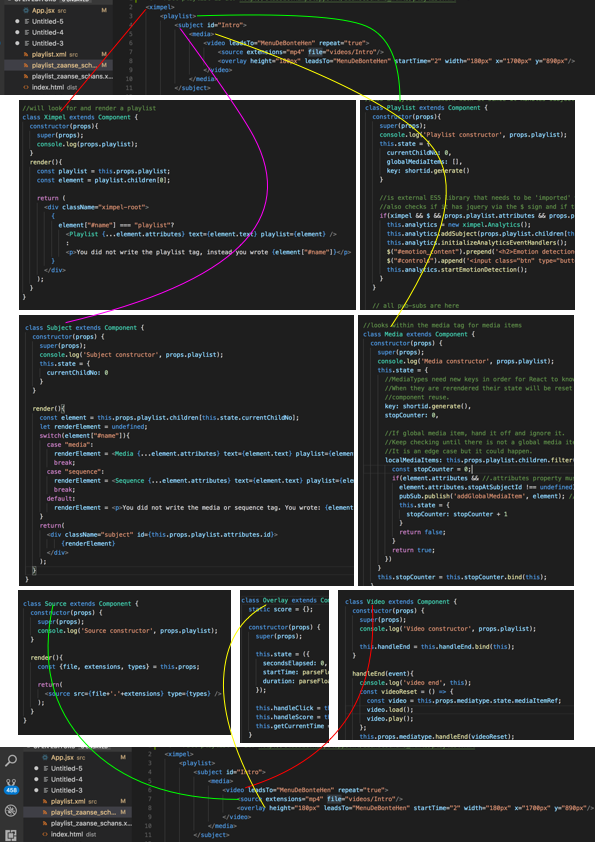
\includegraphics[width=\paperwidth,height=\paperheight]{images/architecture_playlist_to_component_mapping.png}}
%   }
% \caption{test}
% \label{images:architecture_playlist_to_component_mapping}
% \end{figure}
% \newpage


\begin{figure}
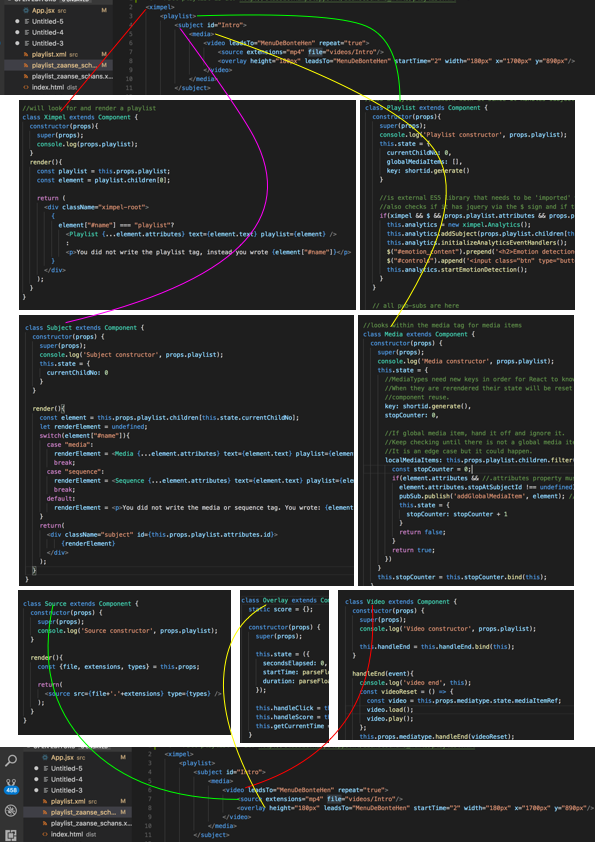
\includegraphics[scale=0.8, center]{images/architecture_playlist_to_component_mapping.pdf} % quotation marks make sure file name does not display
\caption{An example of how a XIMPEL playlist maps onto React components.}
\label{images:architecture_playlist_to_component_mapping}
\end{figure}

\subsection{XIMPEL tags mapped to React component and the link to compiler construction}
To start off this section: consider the following excerpt of the De Zaanse Schans playlist (see code section \ref{playlist:ximpel_zaanse_schans}).

\begin{lstlisting}[language=XML, caption=An excerpt of the De Zaanse Schans playlist., label=playlist:ximpel_zaanse_schans]
<ximpel>
    <playlist>
        <subject id="MenuDeBonteHen">
            <media>
                <video repeat="true">
                    <source extensions="mp4" file="videos/MenuDeBonteHen"/>
                    <overlay height="100px" leadsTo="WalkToHetJongeSchaap" width="350px" x="200px" y="970px"/>
                    <overlay height="100px" leadsTo="QuizBonteHenIntro" width="350px" x="800px" y="970px"/>
                    <overlay height="100px" leadsTo="TourOfMolenDeBonteHen" width="350px" x="1470px" y="970px"/>
                </video>
            </media>
        </subject>
    </playlist>
</ximpel>
\end{lstlisting}

Every tag here as its own React component. The `<ximpel>` tag has the `Ximpel` component, the `<playlist>` tag has the `Playlist` component and so on. 

This design makes it possible to devise rules for every component, just like it is possible to devise rules for every context free grammar when parsing a programming language. Since a XIMPEL playlist is a declarative language, borrowing conceptual ideas from syntax analysis in compiler construction may prove to be useful for describing XIMPEL's architecture.

A context free grammar (CFG) has four elements to it. A set of non-terminals, a set of terminals, a set of production rules and a starting symbol. Of relevance here are the ideas of: non-terminals, terminals and production rules. Knowing which are which tells more about the architecture. These terms will not be used in a strict sense, but the essence of these ideas will remain. When I clearly deviate from the strictness of one of these ideas it will be written in advance. The idea of production rules will be renamed to component rules since the rules of what every XML tag should do is encoded in the React component that maps to it and strictly speaking they are not production rules (though they have some similarities).

The terminals are the easiest to understand: the media items displayed on the web page are the terminals, such as a video element or audio element. These terminal symbols are not strictly terminals in the CFG sense since they can nest elements as overlays and supporting elements (e.g. `<source>` for the `<video>` tag). They are terminating symbols in the sense that the endless nesting stops and a media item will be displayed. Other terminating symbols are: `<source>` (as a part of `<video>`) and `<overlay>` (as a part of any media type).

The non-terminating symbols are: `<ximpel>`, `<playlist>`, `<subject>`, `<media>` and `<sequence>`. Writing a playlist with only these tags will yield in a meaningless playlist.

\subsection{Component Rules}
The component rules are written per React component in the source code. For architectural purposes, I will present the rules per component, but they may not be fully comprehensive. They will, however, serve for having a strong understanding of the architecture underlying the code base. The rules will be discussed from top to bottom. 

\subsubsection{Ximpel}
The `Ximpel` component checks whether the `<ximpel>` tag has been written. 

It sees if there is a `<playlist>` tag underneath it and will output a warning on the page and not render anything else. 

It does not check if there is one `<ximpel>` tag. 

\subsubsection{Playlist}
This component tracks which subject is being played. 

It also tracks all the global media items (media items that survive a subject switch, i.e. a global media type) and renders them if needed. 

It initializes the logging framework the `enableLogging` attribute is set to ``true''. 

It also has two subscribed methods in the publish-subscribe system that XIMPEL React uses. 

It listens to any component publishing a topic on `leadsToUpdate` and it will update its own state to render a new subject. 

It also listens to when a `Media` or `Sequence` component signifies the topic of `addGlobalMediaItem`, in which case it adds a media item to its own `globalMediaItems` array so the media item is able to survive the subject switch. 

It renders the global media items and the underlying `<subject>` tag. If no `<subject>` tag has been specified it will display an error message on the page.

\subsubsection{Subject}
This component looks for the underlying `<media>` or `<sequence>` tag. If it is not there it will display an error message on the page.

\subsubsection{Media}
This component plays media items in parallel. 

It is able to render a `<sequence>` tag or any media tag. 

It will give an error message if no media type tags or `<sequence>` tags are children.

It counts how many of its children have stopped playing and notifies this to the parent. This notification is intended for the `<sequence>` tag. With it, the `<sequence>` tag knows that it is able to continue playing the next media type or `Media` component. If the parent is a `<subject>` then this notification is not relevant.

Before playing it checks to see if its first media item is a global media item. If it is, it will increment the stop counter since the responsibility of a global media item does not belong to the `Media` component but to the `Playlist` component.

When it renders a media tag, it also renders an element that tracks time for the media item as a parent. As of now this is called `MediaType` but it may also be called `MediaManager` later on. Here is a piece of example code.

\begin{lstlisting}[language=JavaScript, caption=An example of how each media item has a general component to manage itself for time tracking (among other things)., label=javascript:media_type_render]
    <MediaType stopCounter={this.stopCounter} {...element.attributes} playlist={element} key={this.state.key + i} render={mediatype => (
        <Youtube {...element.attributes} mediatype={mediatype} text={element.text} playlist={element} />
    )}/>;
\end{lstlisting}

\subsubsection{Sequence}
This component plays a media item (or `<media>` tag) one at a time and will go to the next one when the duration of its current media item is finished. If a media item has no duration specified in the playlist, this media item will be playing it for an infinite amount of time. A `<media>` tag does not need a duration, it only needs to notify the `Sequence` component that it is done rendering all its children.

It will give an error message if no media type tags or `<media>` tags are children.

It counts which child it is playing and whether it is finished playing.

When it is finished playing it will notify its parent that it stopped. This notification is intended for the `<media>` tag so it knows that this component is done with rendering everything. If the parent is a `<subject>` then this notification is not relevant.

When it renders a media tag, it also renders an element that tracks time for the media item as a parent. As of now this is called `MediaType` but it may also be called `MediaManager` later on. 

\subsubsection{MediaType}
The `MediaType` component is the only component that does not have a direct one to one mapping with the XIMPEL playlist. This component applies to all media types and acts a manager for every media type. All media types have a couple of requirements in common which is why this component was created.

It tracks: duration, the amount of seconds elapsed, whether it has to render itself, it also tracks an inner state of whether it should play and the underlying media type and when a media item needs to start playing.

It is able to get information from the underlying media type regarding the amount of seconds elapsed. This feature is also seen in XIMPEL JS, where it has been argued in the comments that the video and YouTube API are better able to track time than the JavaScript implementation of XIMPEL JS itself.

It notifies the `Media` or `Sequence` component when it stopped playing.

It renders overlays that are children of any media type tags. In the general architecture of XIMPEL React it is a rule that an overlay can only be rendered by a media type.

\subsubsection{Media Types}
Most media types simply render themselves, take in the attributes of what was written in the playlist. `Video`, `Terminal` and (in future work) `YouTube` have more than only a call to a render method.

All media types are able to render overlays and overlays are only allowed to be rendered as children of media types.

The `Video` component also tells `MediaType` when it is done playing itself when it is not on repeat and it gives a reference of itself to `MediaType` in order for `MediaType` to improve time tracking (e.g. when a video is paused there is no time elapsing). The `Youtube` component could be programmed to do these things too, but as of now this has not been done yet.

The `Terminal` component connects to a server that runs a bash shell and communicates via web sockets. Because of this, it is able to handle form submission.

\subsubsection{Overlay}
This component has a static variable called `score` which is an object that tracks all the scores that are put as an attribute in the `<overlay>` tag. 

It tracks its own time, except when `MediaType` passes down a reference of the HTML5 video player. Then the time will be tracked for the overlay.

Other than tracking time it also tracks start time and duration.

It renders itself and has no children.

The most important feature of an overlay is that when it is clicked, it will publish a `leadsToUpdate` to any subscriber willing to listen which is the `Playlist` component, since it will start rendering a new `Subject` component, forcing a rerender of a whole new part of the playlist.

% kun je een force unmount doen?
% je kunt een force unmount doen, dus dit zou eventueel kunnen veranderen.
\subsection{Beyond the component rules}
It is important to know that while these rules describe the components fairly adequately, two things have been left unsaid. Certain edge case behavior has not been discussed and lifecycle management issues that needed to be programmed against. An example of one edge case is that the logging framework is written in ES5 and jQuery. Because of this the `Playlist` component needs to check if jQuery exist and use it in order to attach the facial expression classifier part of the framework to the DOM. An example is key management, which is needed for almost any React component out there. If React needs to use deep diffing into the DOM, then the lifecycle methods will be called at unfortunate moments. This is an issue if a new developer does not understand key management and how it influences the lifecycle methods. Currently it is not a problem anymore, but it used to be.

\subsection{Data flow within XIMPEL React}
The data flow within XIMPEL React tries to follow conventional ReactJS philosophy: try to have a unidirectional data flow as much as possible. Which means data flowing from parent to child. However, sometimes this is not possible. If a child gets a state change earlier which a parent also would need to know, then it in some cases becomes difficult to do so. Conventional React best practice suggests to lift state. However, this has not always seemed to be possible, but furthermore it makes code readability worse.

For child to parent communication I used callbacks or render props (through which I could use callbacks). For great great great ... great grandchild communication to the `Playlist` component I used a publish subscribe library called PubSub.js \cite{pubsubJS}. Some people reading this may ask themselves ``why did you not use the Redux library?`` The answer simply is: it was not needed. I know that a lot of developers use the flux architecture for solving data flow communication issues, but this is only needed when current data flow communication solutions become unwieldy. This is not the case for XIMPEL React. It may be the case in the future, when the codebase passes 5000 lines or 25000 lines (who can tell?) and then refactoring will be needed.

% Op welke manier passen questions in XIMPEL?
% React als ecosysteem? Te doen?
% Maintainability
% Is de React codebase zinvol? Voor? Tegen? Eventuele uitbreidingen?
\section{Conclusion}
So who is hungry? It is about time to assess whether porting XIMPEL in React provides a free lunch! The assessment works as follows. First, unexpected advantages and disadvantages will be taken into consideration. Then, the expected advantages will be evaluated by asking: to what extent were positive development factors in reality?

\subsection{Unexpected advantages and disadvantages}
The biggest downside of React was not the library itself but the learning curve of it. The fine-grained understanding over the lifecycle and key management has produced hundreds of lines of code that were ultimitaly unecessary and have been refactored out. Without this fine-grained understanding, more control over the DOM would be nice, as well as knowing when the lifecycle methods would be triggered. Fortunately, it was a learning curve issue and nothing else. 

The pro's of the React and Webpack combination were plentiful. One advantage mentioned earlier is that React components map really well on XML elements of the XIMPEL playlist. Since the component abstraction rarely breaks, it is fairly easy to reason what each XML element is responsible for regarding which React component. 

Another advantage that came to light later on was the lack of DOM manipulation needed. React does this. Normally, a developer needs to be concerned about: state, rendering HTML (most likely with jQuery) and when to render the HTML. With ReactJS the only concerns are having the right state and rendering it, which simplifies reasoning about the whole application since the question of when to render HTML is gone.

One future advantage is when XIMPEL or concepts like XIMPEL will be used for mobile applications. React Native shares a lot of similar code with ReactJS and to port it over to mobile should be possible. One interesting caveat is that mobile applications need to be reviewed by their respective app stores. However, a playlist that is sent over the server does not need to be reviewed. So a technique to extend an app is to create one's own custom declarative language and load it in as a playlist, like XIMPEL does. A related advantage is that it is almost within reach to create mobile apps with XIMPEL. The framework has to be adapted to React Native, which has a lot of code in common with ReactJS, in general.

% https://github.com/Leonidas-from-XIV/node-xml2js
\subsection{Evaluating the expected advantages}
The first pro is that a lot of parsing logic could be done with React and Webpack. This is true, but interestingly enough, not by transforming the XIMPEL playlist to a language that is completely compliant with JSX. The XML loader of webpack had (in hindsight) a strong XML parser that was a good library to use \cite{node_xml2js}. This parser created a workable in-memory configuration object.

Which brings us to the second pro. The virtual DOM would replace the in-memory configuration code. So there is no need to write in-memory configuration code. While it has been tried to use the virtual DOM to replace the in-memory configuration code, this has been tedious -- this has been done in the second attempt. As stated in the previous paragraph, the actual parsed XML tags were used, which provided the in-memory configuration that was needed -- this has been done in the third attempt.

% https://reactjs.org/blog/2016/01/12/discontinuing-ie8-support.html
% https://reactjs.org/docs/javascript-environment-requirements.html
The third pro is that cross-browser support is managed by the maintainers of the ReactJS framework. This is unfortunately not entirely true since the logging framework has not been ported to React. ReactJS itself support Internet Explorer 9 and higher through the use of some polyfills. It used to support Internet Explorer 8, but it has discontinued support since the beginning of 2016 \cite{react_discontuining_ie8}.

The final advantage was a didactic one. Students who want to extend XIMPEL React need to learn a thing or two about ReactJS. This in turn leads them to learn some computer science concepts. It is hard to assess this potential advantage, but since I needed to brush up on my ReactJS skills, I can review which programming concepts I have gained a better understanding of. These are: lifecycle methods, diffing, performance between a virtual DOM and actual DOM, the DOM itself, some basics of functional programming (I did not follow the course in my bachelor degree), the render and state cycle, the lifecycle of a component (it is reminiscent of the iOS framework Cocoa and Cocoa Touch which also has lifecycle methods) and key management (unique identifiers). It could be argued that some of these concepts are also computer science concepts. Regardless of whether it is true, students who want to extend or play with the core of XIMPEL will learn a lot about web development.

\subsection{Concluding the evaluation}
In summarized fashion, the advantages of ReactJS are: no DOM manipulation, XML attributes easily included as props (thanks to a combination of React and the XML parser), strong one to one mapping to the XIMPEL playlist, cross-browser support, strong error reporting, a strong ecosystem, and porting options to mobile and tablet. The strong one to one mapping to the XIMPEL playlist has been very useful for development. Focusing on solely one tag and writing out the component rules for that tag is helpful. Regarding the props of ReactJS, it has not been needed to attach the XML attributes to anything, unlike in XIMPEL JS. The ecosystem of React is perhaps its strongest advantage since it offered easy discoverability for libraries that saved a lot of time, such as the XML parsing library or the ability to write ES6 with Babel. This means: less code to write, an architecture that is fairly easy to reason about, maintainability out of the box and rapid software development options on other platforms. This is a lot. A speculative advantage is that ReactJS might segment its position as a best practice for the web. 

The only downside is that people need to learn it and become proficient in it. Fortunately, the learning curve should not be that high since XIMPEL React only uses ReactJS its core library and DOM library. It does not use other popular libraries from the React ecosystem that invite a learning overhead (e.g. Redux). Hence, the downside is relatively contained compared to other React ports.

Does this mean that we should abandon ship and stop the development of XIMPEL JS? Compared to the development time of XIMPEL React, the creation of XIMPEL JS has also been realized relatively quickly. While I do not have data on the matter, my guess would be that it has been made within 336 to 672 hours of development time. Bruins developed XIMPEL JS for his master thesis, and had (officially) 1004 hours time for the whole thesis. The point is: that is still relatively quick. 

As of now, XIMPEL React is a subset of XIMPEL JS and has a couple of different design decisions. Therefore, no version of the framework replaces the other. The design decisions of XIMPEL React easily shows whether the design decisions taken were a good idea. XIMPEL React has no: pause and resume functionality, quiz tags, constant dimensions (i.e. 1920 x 1080). Some media items have rudimentary video and audio time scrubbing. Preliminary results show that: quizzes can still be modeled; even quizzes with feedback and not having constant dimensions has consequences of the positioning system in such a way that it is identical to positioning web elements. 

To close this chapter, this exploration is a final exploration in disguise. Since it had three attempts, only the first attempt was the actual third exploration which is now in appendix \ref{chap:exploration3_appendix_part1}. The second and third attempt can be seen as the seventh exploration respectively. When I ported XIMPEL to React successfully in my second attempt and fine-tuned it in my third attempt, the first rough draft of everything (including this chapter) was already written and everything else was already programmed. So other than an assessment to see whether XIMPEL could be ported to React, this port also showcases a particular vision of XIMPEL. The other explorations serve as puzzle pieces of programming and design explorations and they serve as an inspiration for this implementation of XIMPEL React.
% 
\chapter{Exploration 4: creating the necessary requirements to measure the frustration of users in XIMPEL}
% Question: how do we extend XIMPEL with data logging? What theoretical knowledge do we need to analyze the quality of experience, engagement and frustration?

At one point while I was playing with XIMPEL I noticed that I found it to be a shame that every playthrough would be forgotten after it had ended. I wanted some form of memory. I wanted some form of logging. I then realized that creating a logging framework and creating a theoretical framework on how to measure frustration with it would be valuable for improving the user experience of XIMPEL. So in this exploration I am finding out what kind of theoretical framework for frustration (and to a lesser extent engagement) we should have and from that framework what the minimal requirements are regarding data capture.

One reason I chose frustration as an important metric for user experience is because it seems that the experience of frustration is still quite misunderstood in academia. Having written earlier about frustration from a psycho-neurobiological perspective, I had the idea that I would be most productive for the academic community if I would resume my work in this area of research. Another reason is: this is my first attempt and experience at answering an artificial intelligence question while having a background in it through other disciplines, which is exciting!


% Why do I start to talk about my measures first and *then* have a literature review?
% Ik laat ook niet de wetenschap zien achter facial expression detection

\section{Justification for creating a logging framework}
% Tell here that you created history graphs and what it is useful for
One justification is: to understand your users. Hugo Huurdeman shows this justification in work that happened at more or less the same time \cite{ximpel_norway_first_article}. In order to understand more about the user experience (UX) that XIMPEL users go through I have created the beginning of a framework that logs data needed for classifying frustration or engagement. Understanding whether a user is engaged or frustrated helps to improve the UX for authors creating XIMPEL presentations. I chose for frustration and engagement because it will give insight into whether a user wants to quit in the middle of a XIMPEL presentation (frustration) or is driven to see all of it (engagement). Moreover, it begs the question: how does one measure and classify frustration and engagement in hypermedia frameworks? For this question I emphasize a focus on frustration, because quitting an application out of frustration is a more urgent problem to solve than to keep users fully engaged. Another question that came up is: does frustration always lead to quitting behavior? The answer to that is no it does not always lead to quitting \cite{roest2015}. A follow-up question would then be: is it possible to differentiate between different frustrations? To which I found a tentative slightly surprising answer by accident.

Since hypermedia frameworks are interactive they have on some dimensions more in common with digital games than with multimedia. A single video does not allow for much interactivity. However, with XIMPEL it is possible to create a point and click adventure game. Therefore, I chose to review the literature on engagement and frustration regarding digital games. A second motivation to do this is because XIMPEL is an intentional intersection between hypermedia and gaming.

My approach for reviewing this literature is as follows: I draw from my own previous literature review, written in 2015 about what frustration and engagement is and add to that review with new research findings. I furthermore, review literature on how engagement but most notably frustration are measured and classified. 
The result of this literature review will influence my choice of measures that I will include in creating a logging framework for XIMPEL. Furthermore, these measures will have a focus on accessible non-customized hardware, which means conventional hardware available on most laptops and tables. Another result is a literature review itself, which is guided for design and not for comprehensive review but because of that an example of bridging literature to implementation.

\section{What is frustration}
% Check to see if there are new articles, otherwise just take stuff from your old thesis.

In gaming, to frustrate a player means to block their progress. Or as Gilleade and Dix state it, it is: ``that which arises when the progress a user is making towards achieving a given goal is
impeded.'' \cite{gilleade2004} In general, players will feel frustrated when they realize that the blocking of their progress has happened. 

% generality of the definition?
Despite that this definition has been made in a gaming context, it seems to be quite general. Studies about completely different topics (e.g. human motivation) give very similar definitions, albeit implicit. Take for example (emphasis by me): ``Recently, it has further been recognized that beyond measuring need satisfaction versus the lack thereof, needs can also be \textit{actively blocked} or the growth potential of individuals, \textit{the frustration of these needs} would elicit defensiveness, ill-being, and even psychopathology.'' \cite{chen2015} Because of this generality, the definition of Gilleade and Dix will be used.

% Probably not include this, but leave it here for an interesting comment: Frustration can refer to no or little progress in achieving goals due to limited skills and strenuous challenges in tasks -- definition of Csikszentmihalyi 1988

% the nuances of frustration
\subsection{Some nuances regarding frustration}
It matters to whom or what the frustration is attributed to. If the frustration is attributed to oneself it will not cause quitting a game. If, however, it is attributed to the game itself (e.g. lag or too difficult AI) or to another person (e.g. the co-player did not perform well in a task) then the player will quit. This is indeed a quite subjective experience. More forgiving players might attribute the frustration more to themselves than to their co-player, for example. In my literature review, I provided some evidence for this claim but the strongest evidence for it has been found in a recent 2017 study about near-misses in Candy Crush.

The near-miss is a form of frustration where attribution of a failure, which was almost a success, is attributed to oneself. The canonical example of a near-miss is a slot machine that almost shows three lucky number sevens, but the third seven goes a little but too far and reaches over the line, leaving itself at the right bottom corner of the slot machine (see figure \ref{fig:near_miss}). 

\begin{figure}
    \centering
    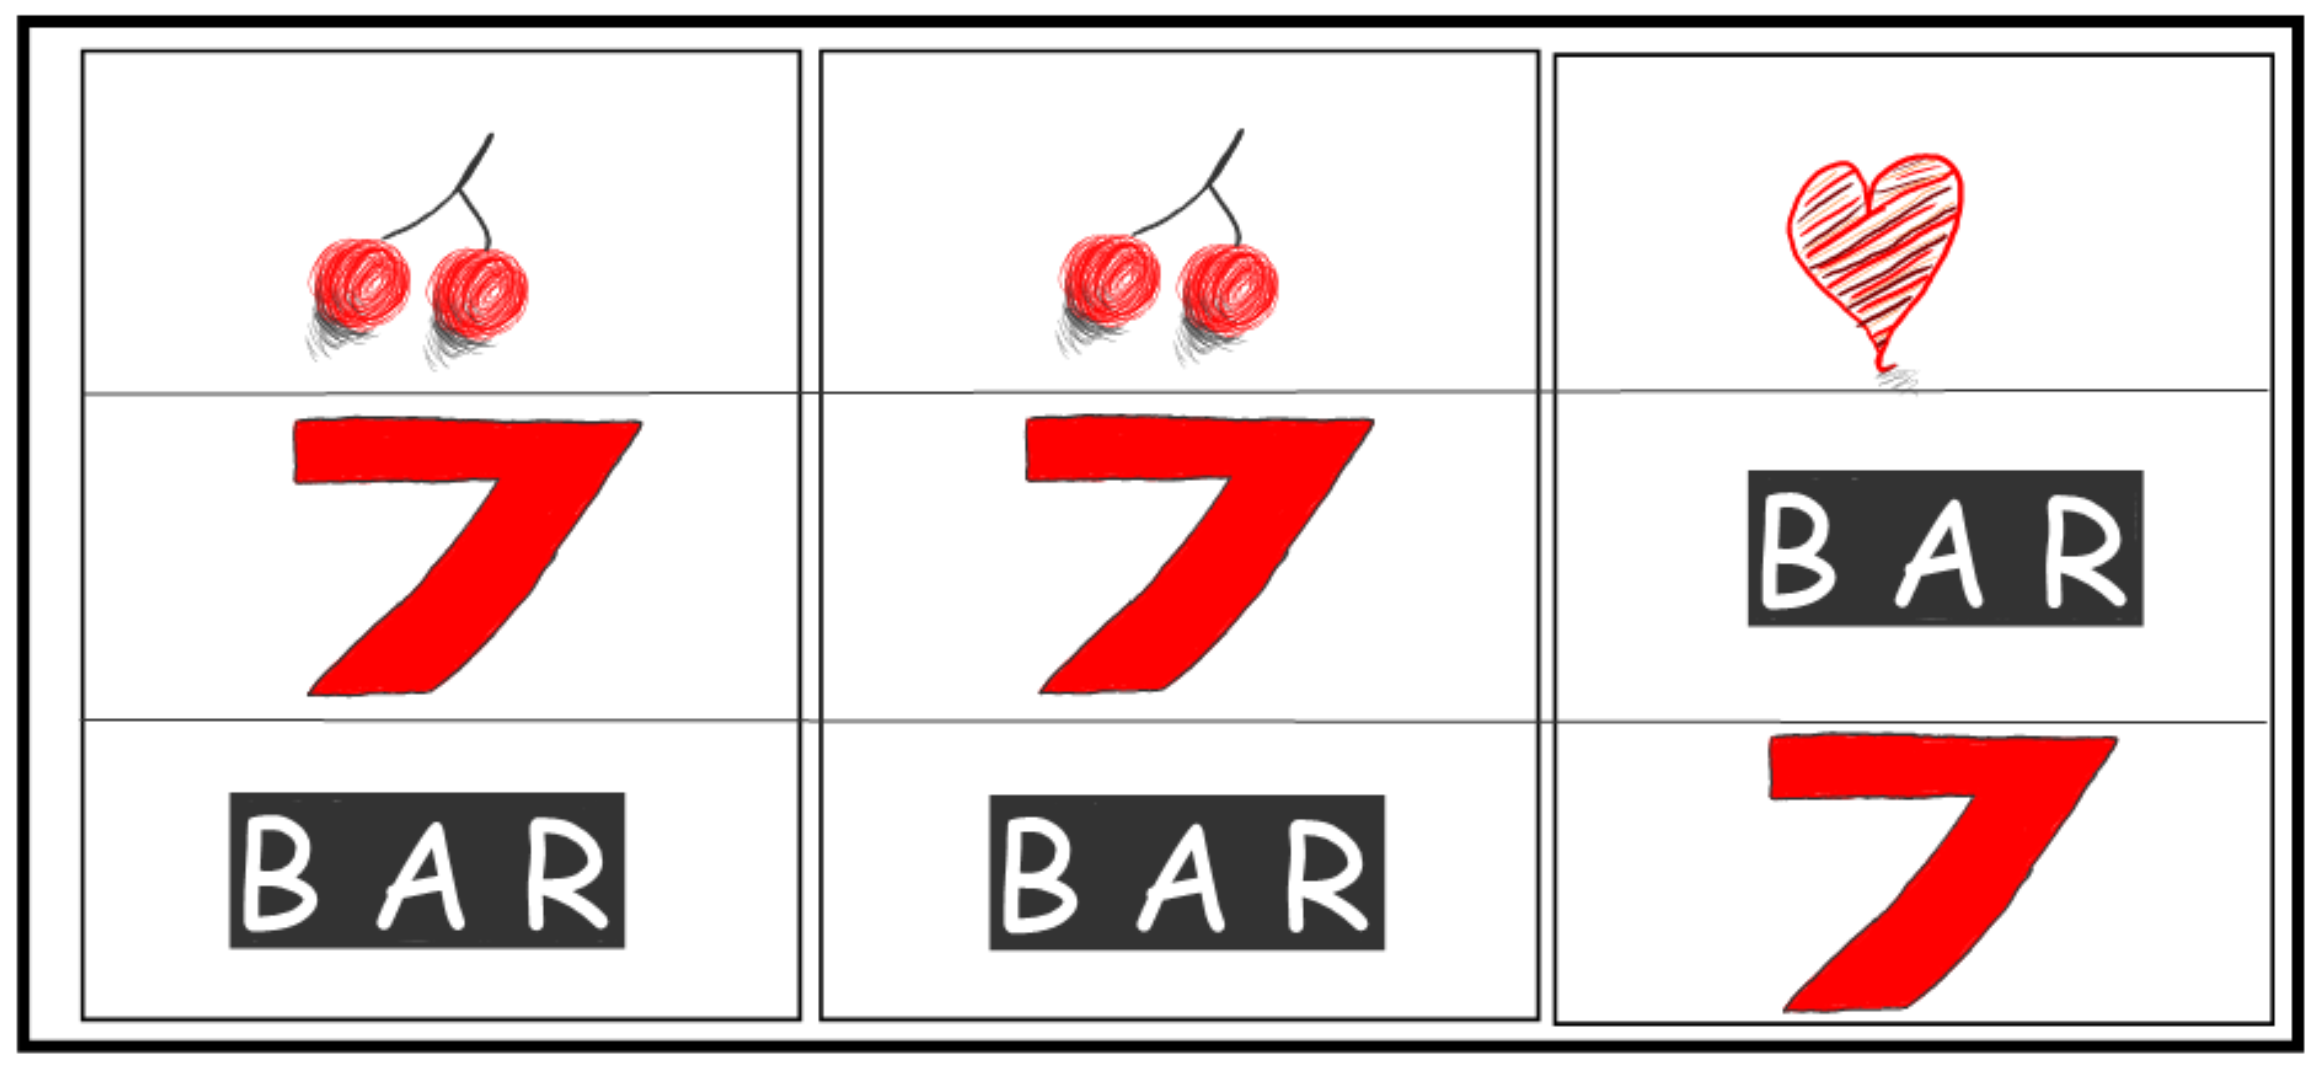
\includegraphics[width=1.35\textwidth, center]{near_miss.png} % quotation marks make sure file name does not display
    \caption{A visual example of a near-miss. The lucky number 7 on the third slot machine column went one place further than intended.}
    \label{fig:near_miss}
\end{figure}

In the study, researchers found that the near-misses in Candy Crush increase the wanting to play and frustration \cite{larche2017}. This is clear evidence for the idea that the attribution of frustration matters since players believe they are able to achieve their goal. For XIMPEL authors understanding this distinction is important when their application resembles a game.

However, when the XIMPEL application resembles multimedia more in the sense of that it is a XIMPEL application in which the user is passive, then the attribution of frustration is in almost all cases on the XIMPEL application itself. When a user is passive, he or she cannot do much in the first place and will therefore most likely place the blame on the application. That blame may be placed on several factors such as: topic mismatch, badly designed applications, the XIMPEL control buttons, or a terrible quality of experience (when watching YouTube videos or other networked media types).

XIMPEL authors need to consider to what extent they deem frustration and the willingness to quit important. In some contexts, frustration matters less. For example, when students are made to watch any presentation during their student lifetime at university, frustration will only lead to disengagement but not to quitting. One might think that this is just as bad, but one study shows this is not always the case. 

Computer scientists at the University of Saskatchewa in Canada created a game to create interpersonal trust in which they showcase: a literature review on what interpersonal trust is, a literature review on how it is developed in real-life and via digital games and an experiment if their game fosters trust. The interesting result is that their game was found to be frustrating. They remark:  ``Our game was strongly affected by networking issues, which made the game more frustrating and difficult than we expected. ... participants in the game condition scored low on competence and high on tension. Comments from the debrief as well as the recordings of the game session confirm that many participants experienced a frustrating, `buggy' game, rather than the playful experience we intended.'' \cite{depping2016} They also state that this situation caused the game to become an out-group and the players to become an in-group, which fosters trust\footnote{I will skim over the fact that they implied on some level that a game is a person (an out-group in this case). Media like games, are social things that we project human values on. Unfortunately, I know too little to academically defend this position and will defer to my media studies and other social science colleagues. These types of things should be discussed more often in computer science literature in order to have stronger assumptions and assertions.}. A game does not have to be fun to reach its designed goal \cite{depping2016}. It could even be very frustrating, it could even be a negative experience. 

% \section{What is engagement}
% % Check to see if there are new articles, otherwise just take stuff from your old thesis.

% % I need to make quite a strong note somewhere on the relationship between frustration and engagement and how it is under
% % https://link-springer-com.vu-nl.idm.oclc.org/article/10.1007/s40429-017-0163-x -- children's motivation to play video games

% https://www.semanticscholar.org/paper/Predicting-User-Engagement-with-Direct-Displays-Us-Arapakis-Leiva/50b73a320e600b841be0bde76be562ac18ca1674 -- maybe check that out for classifying engagement -- all kinds of mouse metrics for measuring engagement and frustration

% Recently an updated literature review about the impacts and outcomes computer games have (2016) has shown more insights into what engagement is \cite{boyle2016} (the older systemic literature review was from 2012 \cite{connolly2012}). In the timeframe of four years, 22 studies done on engagement were deemed acceptable enough for the reviewers. It paints a clear picture how researchers are defining engagement in different ways and some researchers try to move away from the flow theory first formulated by Mihaly Csikszentmihalyi \cite{boyle2016}. 

% The most compelling 


\section{Capturing data for analyzing frustration}
% Just write out and justify what you've created and what is too hard because of time-constraints. Do technically explain how facial expressions get measured.
% Explain here that you could do studies such as correlating facial expressions with mouse movements

Since XIMPEL is a framework with the browser in mind, I have assumed that most users only have access to standardized hardware. This is because at this moment XIMPEL is used by students at the Vrije Universiteit Amsterdam and by organizations who use it in giant tablet installations. Because of time-constraints I used measures that I could only find on my MacBook Pro (2015), since that is the hardware available to me. 

This constraint takes precedence over evaluating academic literature. No organization has given me the tools to do something else and I do not have the funds available to buy specialized hardware. However, some of the reviewed literature (see the next section) does use specialized hardware. Despite this mismatch, these articles provided inspiration nonetheless on the nature of frustration, measuring it or classifying it.

\subsection{Frustration measures: clicks, mouse speed, user XIMPEL subject history and facial expressions}
XIMPEL users tap or click on overlays, which means that taps (not available on my MacBook Pro) or mouse clicks need to be measures. Furthermore, measuring mouse moves at the exact moment when they are made allows for the inference of acceleration or deceleration of the mouse and some estimated average speed in general. Since XIMPEL developers also know on which x and y coordinates their overlays are, they can also analyze through the mouse position if the user is standing on an overlay or media item.

Finally, measuring the starting time and which subjects the users are in at any moment allows for the construction of a path where users have been and for how long. This used to be in the old XIMPEL framework (written in ActionScript) but has not yet been implemented when it was ported to JavaScript.

Measuring: mouse clicks (x, y and time), mouse moves (x, y and time), starting time of playback per subject (in milliseconds) and the subject ID forms the basis of measuring frustration. It is quite unfortunate that these measures are relatively indirect. Frustration is a feeling first and foremost and gets expressed through the user in a variety of ways. 

The need to obtain more direct data was there since these measures are perhaps too indirect to be useful for classifying frustration. Maybe it would be possible to capture frustration through the use of a web cam. While it is not as standardized (or unobtrusive) it may help greatly in the situations in which it can be used. So I decided to make that an optional measure. Sending web cam data directly is a lot of data to store. Therefore, I decided to classify facial expressions directly through the CLMtrackr JavaScript library. It detects: joy, anger, surprise and sadness. It has to be noted that this is a trade-off to make. Does a data capturing server store video streams or does it store classified data? The disadvantage of the former is that there is a lot of data to store, the disadvantage of the latter is that the data contains less information since there is a lot more one can do with pure video data than classified facial expressions. How this classification works is explained later in the chapter. 

The use of CLMtrackr and classifying emotions related to frustration have two reasons. (1) Detecting facial expressions in the browser in general is difficult, so it is better to work with libraries already in place for this. As of writing, this is the only library I came across. And (2) in the reviewed literature on facial expressions (see section \ref{frustration_facial_expression_literature}), there is a strong argument to be made to not measure the facial expression of frustration. To summarize (2): the detection of anger may be useful since frustration and anger are very related through the frustration-aggression hypothesis \cite{roest2015}. Sadness may be useful as well since it can be caused by a hopeless variant of frustration \cite{kuppens2003}.

\subsection{Software architecture and implementation for capturing data}
% Client-server and stored in a database
% Have some screenshots
% Discussion point here: there is double work done on the server-side of things

All the mouse click, mouse moves, starting time, subject ID and classified facial expressions are sent to a NodeJS server. That server created a session ID to the client beforehand (including the date and the time) and stores everything in a postgres database. The data stored can later be retrieved for classification. The reason for not doing it on the fly is because it is computationally expensive and perhaps even wasteful. The detection of frustration is only relevant when developers want to improve the UX of XIMPEL. NodeJS with Express has been used because developing with an unopinionated microframework allows for the quick creation of routes that stores data in a database. The data can be queried from the database using any kind of program. 

Independent parallel work has been done in similar fashion by the programmers of the University of Oslo who develop XIMPEL applications specifically for tablets. Instead of using NodeJS and Express, Python was used in combination with Flask, which leads to a more or less similar communication pattern between XIMPEL and the server-side data capture application \cite{ximpel_norway_datacapture_server}. 

% to do -- maak plaatje hiervoor -- maybe

% Measures
% Facial expressions (angry, sad, happy, surprised)
% Mouse clicks (x, y)
% Mouse moves (x, y)
% Starting Time
% Subject Id

\section{Classifying the measures as frustration} %think about this
% Before you start your own thoughts, look up literature first

Now that we have a way of measuring raw data for frustration, the next question is: how to determine when a user is frustrated with this data? The approach for this is to first look at previous research and then conceptualize a possible classification method.

% It is around this time that I started to ask myself if there had been research on this. And to my surprise there was! This comes as a surprise since the literature on a nuanced view of frustration is rather sparse. So I believed there would not be research that would classify frustration. I was wrong. So while I did already determine my metrics on how to measure frustration, it is only now that I started to read about others who did the same.

I do need to note that I did not implement a classification algorithm. It is outside of the scope of this project to implement it. However, conceptualizing a first iteration of such an algorithm or algorithm design approach leaves opportunity for further realization in future work.

\subsection{Related Literature}

% input --> AV-space --> emotions
% Do I need images or diagrams for this?
\textbf{Depping, Mandryk, Johanson, Bowey and Thomson} used four inputs (galvanic skin response, heart rate and EMG frowning and EMG smiling) in order to calculate arousal and valence values. A certain combination of arousal and valence (which is a range from displeasure to pleasure) would yield a particular emotional state: boredom, challenge, excitement, frustration, and fun. Each input is a time series that would be used to create a time series for arousal and valence, called AV-space (figure 1, 3, 14 and 15 in their paper \cite{mandryk2007}). 

For example, increasing galvanic skin response would be mapped to increasing arousal. Low or high galvanic skin response would be modulated with heart rate data, where a low heart rate would result with a lower arousal level than high heart rate data. EMG Smiling would mean that valence levels increased and EMG frowning would mean that valence decreased. They had other rules which have been written in more detail in \cite{mandryk2007}.

Then, they created a mapping from AV-space to emotions. In particular, frustration needs to have a high arousal (e.g. high galvanic skin response and high heart rate) and low to medium valence (i.e. displeasure, e.g. frowning on the EMG). They discuss all their emotional states in their paper \cite{mandryk2006} and go into more detail in another paper \cite{mandryk2007}. Through a user study they found that their predicted model of frustration did not coincide with self-reported frustration. This was not the case with for the emotions fun and excitement \cite{mandryk2006}.

% Picture would be nice, since it makes it easier to understand

% Cogni Mouse
\textbf{Researchers in Cyprus and Portugal}\footnote{To make it a little bit confusing, one of the researchers is called David Portugal. His last name and the name of the country Portugal bear no affiliation. Jo\˜ao Quintas is the researcher who is affiliated to a Portuguese laboratory.}, created a new mouse called CogniMouse\cite{portugal2016} for older computer users. With this mouse they hoped to measure frustration since some older computer users have some difficulties using computers at work. While I am not developing my own computer mouse, it is interesting to see which extra measures the research team was trying to get. The sensors in the mouse are a: ``galvanic skin response sensor, temperature sensor, inertial measurement unit (IMU), grip/pressure sensor, and heart rate sensor.'' \cite{portugal2016} They used a classification algorithm that employs ``Bayesian-based formalism inspired on conditional probability distributions.'' \cite{portugal2016} This means that they used a formula that constantly calculated a probability to what extent the user was frustrated. They used: grip force, acceleration vector and click stream frequency as inputs. The formula itself is:

$$P(Frus|Grip,Acc,Click)=\dfrac{P(Frus)*P(Grip|Frus)*P(Acc|Frus)*P(Click|Frus)}{P(Grip)*P(Acc)*P(Click)}\cite{portugal2016}$$

The formula clearly shows the Bayesian nature of the classifier. They have a planned user study and present a use case scenario of a middle aged woman who would experience issues using a new computer system. The CogniMouse noticed her frustration and helped her by presenting a graphical help wizard. In their future work they will add more ways to track the user, such as an eye tracker.

% measuring frustration in keylogs in a programming course
% using bayes method to detect frustration with keystrokes, mouse strokes and interaction logs
\textbf{In the study of \cite{leong2016}} an annotator annotated the signs of frustration from web cam recordings, where students in those recordings made use of web based programming tutoring meant for a Java programming course for beginners within University of Singapore. Students mouse clicks, keystrokes and actions were written into log files. This was compared to the annotations on a time scale. After this comparison, relevant extracted metrics were: ``the mean and median key latencies, number of keys, wait time (duration longer than 1 second with no key inputs), back space and delete key latency and frequencies and the frequencies of mouse clicks. The interaction features include the number of compilations, number of errors encountered, number of exercises completed and the duration of time spent working on the exercises.'' \cite{leong2016}

The extracted features were aggregated into a sliding window with sizes of 30, 60, 90, 120, 150 and 180 seconds; where windows would overlap each other for one-third of whatever window size was determined. Frustration would be observed per sliding window. If the frustration occurred in the overlapping sliding window part, then both sliding windows were annotated as a frustrating event. Changing the window width from 30 seconds to a 180 seconds -- and everything in between -- would have consequences for the detection of frustration. If someone gets frustrated within every 3 minutes, then a window size at the highest width would always be marked as frustrating, this would not be the case for lower window width sizes. The problem with lower window width sizes is that there might be insufficient data to determine anything at all.

To classify frustration within these sliding windows they trained a Bayesian network and compared it to a naive Bayes model. The performance of the Bayesian network compared to the naive Bayes model was a significant improvement. The performance improvements were 32.79\% (under the curve, they authors did not define what this means), 32.73\% (accuracy, ``the number of correctly identified instances divided by the total number of instances'' \cite{leong2016}) and 2.53\% (sensitivity which ``measures the true positive rate or the proportion of positives that are correctly identified as such while specificity measures the proportion of negatives that are correctly identified as such'' \cite{leong2016}).

% Stress on e-learning students
\textbf{Instead of classifying frustration, one could also classify something else such as stress}. Rodrigues, Gon{\c{c}}alves, Carneiro, Novais and Fdez-Riverola did this \cite{rodrigues2013} in a study for which they created a stress detection tool in for the e-learning platform Moodle. They created a system called the Dynamic Student Assessment Module (DSAM) which has all kinds of components for detecting the mood of a student. The DSAM does this in two ways: by asking students through a questionnaire and by looking at their behavior. They looked at their behavior through ``facial analysis, mouse analysis, keyboard analysis, and log analysis (through Moodle logs).\cite{rodrigues2013}'' The features they analyze are: ``the number of mouse clicks per minute, the average duration of mouse clicks (from the button-down to the button-up event), the maximum, minimum and average mouse speeds, the keystroke rate (strokes per second), the average duration of a keystroke (from the key-down to the key-up event) and performance measurements.\cite{rodrigues2013}'' They asked 10 students to do two similar programming tasks. In one programming task they were stressed through the use of a time limit and being told that this assignment was very important for their future (academic) career.   They found that the following JavaScript events were fired a lot more when students were stressed: key down, key up, mouse down, mouse up, mouse wheel and mouse movement. In some cases it was 5 times as high, in other cases about 1.5 times as high. From these differences they claim they can detect stress.

\subsection{Proposed approach for classifying frustration in XIMPEL}
In the related work section a lot of input sources have been described (too many to list). Classification techniques were: rule-based, Bayesian and comparing it to a control group. Furthermore, \cite{mandryk2006} wrote about another author using Markov chains. It seems to be the case that any probabilistic classification technique can be tried. Other than probabilistic classification techniques, rule-based techniques sometimes seem to work -- comparing results to a control group is a specific example of a rule-based technique.

In XIMPEL we measure: mouse clicks, mouse moves, a historical trail (with time) of which subjects a user goes to and facial expressions. Since a hypermedia-like application could be different than a game or a generic application due to watching video, some measurements will not always be the same. For example, someone could get frustrated at miss-clicking on an overlay, finally the user will click on the overlay. Compared to a non-frustrated user, the frustrated user will likely have more clicks. But if a user is frustrated because a certain video is boring and he or she cannot go to the next subject, the frustration may only show via their facial expression and not through their use of how they use the computer mouse.

Since it seems more important to give insight to XIMPEL authors when a user is \textit{possibly} frustrated, I put more emphasis on detecting all true positives. In order to detect all true positives, one must be willing to accept that there will be possible false positives. In order to get all true positives one must minimize false negative occurrences of frustration and thus be forced to have more false positives. At the same time, looking into a particular possible frustrating episode must be worthwhile so having a signal to noise ratio of 10 to 1 might be a bit much since it might take 2 to 5 minutes to check a possible occurrence of frustration (e.g. checking the data for a particular person for a possible frustrating occurrence). A signal to noise ratio of 1 to 3 would be much more acceptable. For example, if the signal to noise ratio is 1 to 3, then it would take 20 minutes at worst to look at instances of possible frustration.

So the requirements for our classifier are:
\begin{itemize}  
    \item A signal to noise ratio of 1 to 3 or lower (specificity).
    \item If the first requirement is not broken yet, then get more, or even all, occurrences of frustration (recall).
    \item Be able to pickup on frustration when the user is not using computer peripherals (e.g. listening to audio or watching a video).
    \item Be able to pickup on frustration when the user is using computer peripherals.
\end{itemize}

Time constraints prevent me to create such a classifier. Nevertheless, I will write my ideas down for future work related purposes. Since interactive video, hypermedia and XIMPEL applications are a bit different than other applications, an observation study should be done as to what makes users frustrated. From such an observation study it should be possible to see what frustrated behaviors users have and how this could be possibly measured. The measures that I programmed for are a mix of a best guess inspired by literature and hardware constraints.

Classification should depend on the requirements for detecting frustration within XIMPEL. These requirements are listed above and were made with the rationale of why we should detect user frustration within XIMPEL applications in the first place which is to improve UX. The requirements are fairly broad, which means that a potential solution does not have to be perfect. It is likely that multiple solutions are possible.

My approach to classifying frustration would be to create a simple classifier per input type. So there is a mouse movement frustration classifier, for example, and also a facial expression frustration classifier. If one of these classifiers gives an alert, then frustration is possibly detected. This is possibly too straightforward, but it allows to get more experience as to which input types explain frustration independently from the other input types. Testing which classifiers give too many false positives is future work. The question that I will attempt to answer now is how does each classifier work?

While this is one question and directly applies to mouse clicks, mouse moves, user trials and time between subjects; it applies differently to detecting frustration in facial expressions. CLMtrackr already classifies facial expressions. So the question regarding facial expressions goes much deeper and this depth is written down. Then, I realized that in my first literature search on detecting frustration in users I did not find anything about how to detect frustration in facial expressions, so I did a separate literature search for that specific question. So the specific questions regarding frustration in facial expressions are: (1) how does the current classification algorithm work regarding basic emotions? (2) do classified basic emotions help classify frustration, if so, how? And (3) why not detect frustration as a facial expression directly? Perhaps noticeable, questions 2 and 3 are related to how does the facial expression classifier work?

\subsubsection{Facial expressions}
% Anger --> frustration
% Sad... ?
% Happy, surprise --> engagement
% Leg uit waarom je voor een proxy moet gaan
The JavaScript library CLMtrackr classifies anger, sadness, happiness and surprise and gives all four a value between 0 and 1. 
CLMtrackr does this through constrained local models (CLM) among other things. It technically also classifies contempt and fear but not good enough according to a quick discussion with the CLMtrackr author on the Github Issues page \cite{github_issue_clmtrackr}, which is why these facial expressions are not classified. CLMtrackr trained its facial recognition abilities through the MUCT Landmarked Face Database (MUCT: Millborrow -- the author -- University of Cape Town)\cite{milborrow2010}. This database has 76 points (called landmarks) annotated on 3755 faces. It is possible to see an example image of such an annotated face on their homepage \cite{milborrow2010}. 

What follows now is a high level explanation of how this works. However, the mathematics will not really be explained since they have been explained quite well in the online resource of \cite{auduno2014}, which I recommend to anyone interested in the technical details of facial detection. That article also points to amazing resources on CLM itself.
The algorithm that Clmtracker uses is called subspace constrained mean-shifts, which is a form of a CLM and is authored by \cite{saragih2009}. CLM algorithms in general have two strategies that happen iteratively until some optimum has been found as explained in \cite{saragih2009}. 

\begin{itemize}
    % \item 1. perform an exhaustive local search for each PDM landmark around their current esti- mate using some kind of feature detector
    % \item 2. optimize the PDM parameters such that the detection responses over all of its landmarks are jointly maximized.
    \item 1. Exhaustive local search: perform a local search for each landmark in the model around their current point estimate. Use a classifier that will generate a probability map and associate the landmark to the highest probability pixel on the map.
    \item 2. Optimization: it could be that some landmark to pixel associations are a bad fit because there were no high probability pixels on the map. Shift their point estimate to somewhere else by calculating where there are likely higher probabilities.
\end{itemize}

The mathematical techniques that make this possible are explained below. I do have to caution the reader that I intuitively understand what is happening, but I do not understand the mean-shift algorithm and associated algorithms well enough to explain its details. Such details can be read in \cite{saragih2009}. Furthermore, data cleaning techniques that are used are not presented at all in this thesis (see \cite{saragih2009}).

The author of CLMtrackr built a model through the use of Principal Component Analysis (PCA), which informally speaking is a method by summarizing as much variance into a component. This is done by first calculating the mean points of all the landmarks of all the annotated faces, then PCA is used to extract the variations as components (they can also be seen as linear combinations of vectors). PCA has the property that the first component accounts for the most variance, the second component for the second most variance and so on. This means that with a few components most variance has been accounted for. PCA is therefore really useful as a data summarizing technique. The components themselves are uncorrelated to each other\footnote{An in-depth mathematical student explanation on can be found on \url{http://www.cs.otago.ac.nz/cosc453/student_tutorials/principal_components.pdf}. The best visual explanation about PCA is to be found here: \url{http://setosa.io/ev/principal-component-analysis/}. The best visual explanation for eigenvectors is here: \url{http://setosa.io/ev/eigenvectors-and-eigenvalues/}.} The PCA model of a generalized face can be viewed at \cite{clmtrackr_model_viewer}. Playing with it gives a better intuitive understanding of what PCA does regarding finding the average model of a face and the variations of that on a per component basis. 

The model has 70 points. Each point in the model has been associated to one classifier during training, meaning there are 70 classifiers for the model in total. Each classifier has been trained by cropping a small patch of its associated annotated point per facial image (3755 facial patches per annotated point in total). The classifier for such a patch is a logistic regression classifier with a support vector machine linear kernel (and a MOSSE filter which is of less importance). The reason it is a logistic classifier with a linear kernel\footnote{The author Audun Mathias Øygard calls it an SVM kernel. However, digging into the source code it seems that the so-called SVM kernel is a linear kernel. I had to dig deeper since there is no such thing as an SVM kernel. The kernel can be seen here with a search query in the Github repository: \url{https://github.com/auduno/clmtools/search?utf8=\%E2\%9C\%93&q=kernel}} is because it ``is what the original paper suggests.'' \cite{auduno2014}

\textbf{Exhaustive local search.} When the classifiers are used it crops a local (i.e. small) search rectangle around its initial position and calculates a probability map of pixels which are aligned with the landmark. When this works, such a map has a few high probabilities lying around in the center, of which one of them is the highest and that pixel value (or grid of pixels) will be associated to the landmark. This is done for all 70 landmarks in the model. 

\textbf{Optimization.} However, doing this there is one problem. Since the local rectangle might be too local. The problem with this is that some classifiers cast their local rectangle in a different area compared to where the actual facial feature is (e.g. an eye). In order to counter this, a second step is being done that is akin to gradient descent. This is done by shifting the point of a landmark, which means when it will cast a new rectangle to search for the highest probability it will find new values. The method is called a mean-shift. This mean-shift is determined by using expectation-maximization.

By doing all of this we have found faces. What we have not found are facial expressions. These are classified using logistic regression. The parameters of the facial model are used as features. To get training data for the regression, images of people expressing emotions have been annotated and projected on the PCA decomposition. By doing this, the closest parametrization is achieved. What is not done but could be done for future work is to first determine a neutral baseline, since it is not clear how expressive emotional faces are beforehand. The emotion classifier can also be viewed since the regression coefficients can be used as parameters for the facial model. You can view it at \cite{auduno2014b}.

\subsubsection{Detecting frustration through CLMtrackr}
The facial expression of anger is interpreted as frustration. The facial expressions of happiness and surprise is interpreted as its opposite: engagement. Sadness might be a meaningful measure of frustration as well since it has shown to correlate as much to frustration as anger \cite{kuppens2003}.

It is important to keep the classification of engagement since it may give extra data if another classifier does classify that the user is frustrated. In most cases facial expressions should take precedence over mouse clicks, mouse moves and history graphs because a facial expression conveys how a user feels, much more so than the other measurements. The reason for that is that facial expressions are much more connected to emotions than the other units of measurements since facial expressions are a display of emotions.

% Not included in this thesis:
% https://www.paulekman.com/blog/anger-problem/
%% Reason: blog post and no sources

% https://www.paulekman.com/blog/respectful-disagreements/
%% Reason: blog post and no sources

% https://journals.lww.com/nursingresearchonline/Abstract/2010/05000/A_Meta_Analytic_Study_of_Predictors_of_Anger_in.4.aspx
%% Reason: I'm lazy, site does not load and I need to get this done

% ---

It may seem a bit of a cop out to use anger and sadness as a proxy of frustration. However, perhaps it is not. Anger is the result of a particular frustration. When a user is frustrated at anything other than him or herself, he or she will become angry \cite{roest2015}. Therefore, the detection of anger is a possible detection of frustration. Other research (not included in the literature review) that point to this direction is research about consumer anger \cite{funches2011}. The authors do not explicitly write about frustration, but in this study all the sub-categories of anger are related to frustration in the conceptual sense, they are: broken promises, unfairness and expressed hostility (by service employees to customers). Neuroscientific research shows that ``poorly controlled frustration, manifested as exaggerated anger.'' \cite{yamagishi2012} Research on emotion regulation implies the same, in one paper it is stated that ``a low frustration tolerance is related to trait anger and a higher level of frustration tolerance is related to lower levels of anger and longer persistence on difficult tasks.'' \cite{szasz2011} 

Kuppens, van Mechelen, Smits and de Boeck gave strong nuances to this view. In their article the appraisal basis of anger was evaluated to which components were necessary and sufficient. The researchers conducted two studies and they found that ``other accountability and arrogant entitlement, as instance of unfairness, are specific appraisals for anger.'' \cite{kuppens2003} They suggest that frustration and having an antagonistic action tendency co-occurs. This is easier to believe for having an antagonistic action tendency, since only one study found an association with anger. However, the reason they state for the feeling frustration leaves much to be desired. They studied the \textit{feeling} of frustration in their first study and \textit{goal blocking} in their second study. They found that goal blocking is not associated with anger but feeling frustrated is. They also found that feeling frustrated is associated with sadness \cite{kuppens2003}.

Putting anger and sadness side by side from their first study, it is observed that sadness has frustration as an appraisal-action tendency component and did not have any significant correlation with the other appraisal-action tendencies. Interpreting these results it could mean that sadness occurs when one feels hopeless because of frustration. Whereas if one feels angry because of frustration it is because of someone (or perhaps something) else. 

The result of Peter Kuppens et al. give an indication that indicators on sadness may be important as well. Therefore, the final conclusion of detecting frustration in facial expressions is that sadness and anger combined are an interesting proxy for frustration and joy and hope for engagement.

\subsubsection{Detecting the facial expression of frustration}
\label{frustration_facial_expression_literature}
The complexity of writing a thesis while programming is that a program can become obsolete when new literature is found. It is quite possible for a researcher to believe they are up to date for a certain topic, only to discover there was extra information out there available by a slight alteration of their search queries which they had not considered. This arguably happened for this project, or perhaps not. Indeed, an exploratory thesis such as this one is quite prone to requirements creep. Additional found literature seemed to answer one particular question: how does one detect the facial expression of frustration directly?

The following articles have not been found initially, because the importance of detecting facial expressions at all -- on a practical level -- had more importance. Both studies used the Facial Action Coding System (FACS) which divides the face up in certain sections. These sections are called action units. Humans code these action units on a 1 to 5 point scale in terms intensity. These 5 points are labeled as: (1) trace, (2) slight, (3) marked or pronounced, (4) severe, (5) maximum. Other modifiers are R and L which convey information that assymetrical movements happen on the right or left side of the face. 

In one article action units (AUs): 1, 2 and 14 (14 is of secondary importance) were associated with frustration. AUs are respectively named after their movements. For example, AU 1 is called the inner brow raiser, AU 2 is called the outer brow raiser and AU 14 is called the dimpler. Moreover, action unit 1 and 2 often occured together and ``triggered each other'' \cite{craig2008} which means that ``a raised inner brow tends to trigger a raised outer brow, and vice versa.'' \cite{craig2008}

An article written five years later (in 2013) compared the results of the authors of \cite{craig2008}, though not specifically from the paper that is outlined in the previous paragraph but a paper written by the same authors a year later \cite{craig2009}, which describes two studies one of them being the study of \cite{craig2008}. They found completely different results since they noted that frustration has a strong association with AU 4. They note that AU 1 was associated with whether a student self-reported their tutoring session (with JavaTutor) to be worthwhile. AU 2 was associated with whether a student self-reported the feeling of being rushed during a tutoring session. AU 14 was was associated with whether a student self-reported with whether how successful he or she felt in the accomplishment of a task. All the AUs they found for their dependent variables were: AU 1, AU 2, AU 4, AU 7 and AU 14. They measured self-reported frustration as: ``How insecure, discouraged, irritated, stressed and annoyed were you?'' \cite{grafsgaard2013} It could be the case that they measured something different than frustration since: ``discouraged, irritated, stressed and annoyed'' is not particular to only frustration, whereas the other questions in their post-session survey seem to be related to frustration. The authors note a similarity with how they detected AU: 1, 2 and 14; with its relationship to frustration in previous research as well. They seem to suggest that these action units are related to frustration. Finally, their research shows how difficult it is to replicate previous research in this area.

This difficulty is also seen in the final article found for this section, which has been peer-reviewed but will be published later in 2018. The topic of research was detecting frustration in frustrated drivers. In this study the authors found that they were mostly in line with the action units that also have been found by Ekman, which are AU: 4, 14, 23 and 24 \cite{ihme2018}. These action units are only partially in line with research from the previous paragraphs written. The authors from the previous paragraphs found evidence for AU: 1, 2 and 14 \cite{craig2008, grafsgaard2013}. The authors of \cite{ihme2018} note that these action units have been linked to other emotions such as surprise (AU 1 and AU 2)\cite{ihme2018}. In their final results they found no significant result for AU 4 and AU 14. They did find a significant result for the association of AU 23 and frustration. They also did find a significant result for the association of AU 24 and frustration. They furthermore did an exploratory analysis, meaning they also looked between a difference of their control condition and experimental condition while considering all the other action units. In this analysis they found that AU: 10, 12, 17 and 20 also had significant differences between the experimental and control condition.

It could be that frustrated driving does not capture the same type of frustration as a facial expression compared to computer-mediated learning -- which the other two studies in this section were about. It could be that there are issues with the methodology. What it at the very least shows is that finding the facial expression of frustration directly might be possible for specific domains, such as computer-mediated learning or frustrated driving, but it proves to be much more difficult for detecting frustration as a facial expression in general. 
% This does assume that the criticisms outlined in \cite{ihme2018} about frustration in computer-mediated learning is false, which it may not be.

Since it may or may not be possible to directly detect frustration it may seem to be a better idea to stay with the idea of having proxies for frustration such as anger and sadness. Anger and sadness as facial expressions have been studied more in-depth compared to frustration. While it will increase the signal to noise ratio, it is better to have a signal at all since research on finding frustration directly argue on what the signal is. User studies would need to be done to show if this approach has any merit.

\subsubsection{Mouse clicks and mouse moves}
% Frustration: aggressive movements
% Engagement: ??
In XIMPEL a user navigates with the mouse either to interact with the XIMPEL presentation (through overlays, form input or multiple choice questions), to use the XIMPEL controls (stop, pause and play) or to use a feature of the browser they are using. By being aware of this, it is obvious that a classifier for mouse clicks and mouse moves is only able to detect frustration when the user interacts with the video. This frustration is hypothesized to occur in two ways. 

The first one is that for some reason an interactive feature of XIMPEL does not fully work. For example, a user types out their nickname in the XIMPEL application and when the user clicks on submit nothing happens. Sometimes this can happen in any application and most users would click again. Yet, if nothing happens, the chance of frustration is really high since the user is not successful in reaching his or her goal. In the data one would see a lot of mouse clicks and little mouse moves at the same location. This form of frustration is obviously UI-frustration and is possibly as easy to classify by filtering the data for a lot of mouse clicks on the same place. If a lot of users have issues at the same location, then it is abundantly clear that the UX need to be improved.

The research of \cite{rodrigues2013} showed that there was more mouse movement, mouse down and mouse up events when programming students were stressed. Programming is a more interactive experience than a hypermedia presentation so not all metrics may show up in the same way when it comes to hypermedia presentations. However, having experienced hypermedia presentations myself, one hypothesis is that it could be the case that mouse movement is more rapid in a frustrating experience compared to a non-frustrating experience. In these cases a user feels he or she is waiting too long for going to the next subject. This is a form of content-frustration -- arguably also UI, since there is no time-scrubbing. 

% It could also be the case that users click on something since they thought it was something else?

\subsubsection{User trails and time between subjects}
% Frustration: ?
% Engagement: went on an exemplary path with exemplary times as the multimedia author intended it

When it comes to analyzing the history graphs, the most important questions to ask are: (1) did the user spend the amount of intended time for each XIMPEL subject? And (2) if the user did not, then did the user follow an acceptable trial within that graph? It could be presumed that users feel relatively engaged when they follow a XIMPEL presentation as intended as opposed to when they do not. For example, some XIMPEL presentations present overlays within any subject for the reason that a user can always opt to go to the next subject. This is to alleviate frustration, but in some presentations this is also a problem, depending on the intent and structure of the presentation. Some XIMPEL presentations intend that every piece of content is read and seen and some XIMPEL presentations do not. For those that do, the second question seems more relevant. 

An example of this is the Zaanse Schans (a place in The Netherlands) example on the ximpel.net, where it is possible to do quizzes for every informative video shown, but users are also able to skip them. The intended message would be a bit lost if users did not take the quiz since that helps for memory retention. However, it could be argued that it is acceptable that all quizzes were not experienced by users as long as they view al the video content. If users do not view all video content and quit prematurely, then that may be seen as a sign of frustration.

User trails and time between subjects have two questions that seem quite XIMPEL presentation independent. This is another reason why frustration classification has to be done after the fact since acceptable paths and acceptable times can only be determined after a story graph and design of a XIMPEL presentation is finished. Moreover, the idea of what is an acceptable history trail and time between subjects may change in the mind of the XIMPEL author. This could be even years later. For example, a new improvement for the XIMPEL presentation may be added and it changes the idea of what is an acceptable history graph.

\subsubsection{Conclusion}
% Je mag ook zeggen dat dit niet allemaal geautomatiseerd hoeft te worden gevalideerd, maar dat een interpretatie van een developer of UX designer ook prima is
The philosophy of XIMPEL is being pragmatic. In this case the pragmatic approach is to classify certain features that I am able to do and for other features I offer my best approximations of it. It would be best if frustration could be automated, but in detecting frustration for XIMPEL it would be as interesting to be able to filter data instead of full classification. This approach that you do not let the computer do all the work is an approach in AI-based game-design as well (e.g. see \cite{karavolos2015}). 

The approach that I outlined is to create a simple classifier per input type. Having multiple classifiers being good at one type of classification is not uncommon since that is also part of the algorithm regarding how facial expressions are classified \cite{auduno2014}. The input types are: facial expressions, mouse clicks, mouse moves and user trails per subject (how long have they been at each subject in a XIMPEL presentation?), also called a history graph. My approach for facial expressions is to detect anger and sadness as a proxy for frustration and joy and surprise as a proxy for engagement. A baseline needs to be determined, since it could be the case that the classification of certain facial expressions could have high values already at baseline (e.g. 0.8). The suggestion for mouse clicks for detecting frustration is (1) local and frequent clicks; (2) faster mouse moves. For mouse clicks, a baseline needs to be determined beforehand to see the normal frequency of clicks and speed of mouse moves. Detecting frustration in user trials seems not possible but dissatisfaction may be. The outlined approach is to see if the user (1) spends the intended amount of time per subject and (2) follows a trial deemed acceptable by the author. If this is not the case, then the user might be dissatisfied, especially if other classifiers point towards frustration. It most likely is a thesis in itself to implement this fully and do a user study on it.

% to do: describe the others as well and then think of where you want to go with the conclusion. Future work
% oh wait it is a subsubsection for classifying XIMPEL. You have to reread this maybe...

\section{Future work} %think about this
% Explain here that you could do studies such as correlating facial expressions with mouse movements but then in more detail
Future work could be done in various areas. There are a couple of areas of improvement. These are (1) detecting frustration and engagement directly, (2) researching the associations between mouse moves and mouse clicks with facial expressions, (3) improving the classification abilities of the current approach (e.g. better facial expressions detection), (4) implementing the current approach in code and (5) rewrite the unique parts of the NodeJS server-side application to Python with Flask and merge it with the Microtiks server made by Hugo Huurdeman and Dan Michael O. Heggø (the data capturing server made for XIMPEL in Norway). Some of these opportunities will be outlined more in-depth.

% From the definition of frustration, I presented evidence that not all frustration leads to quitting behavior. However, it always is experienced as a negative feeling. This means that 

\subsection{Detecting frustration directly}
% (5) researching to what extent each classifier could make predictions about frustration or engagement on a fundamental level.
Research on detecting frustration directly is tough. There are different experimental outcomes with detecting frustration through facial expressions \cite{craig2008, grafsgaard2013, ihme2018}. One outstanding question that generates more questions than answers is: to what extent is frustration a universal emotion or facial expression? Many emotion researchers claim it is not a basic emotion \cite{ortony1990}. Is it then universal in western or eastern cultures? Or are there even too many differences per country? Or is it even the case that frustration, as a facial expression, is only measurable per topic? Maybe frustrated drivers look differently compared to frustrated programmers.

If the extent of the universality or lack of it is unknown regarding frustration, then research on detecting it will be more difficult to compare. Assume that it is true that the facial expression of frustration is different per topic but researchers do not know this. Then, it could be the case that researchers on frustration simply think that other frustration researchers that study frustration through another topic are simply wrong. Just assuming that frustration has some form of universality is assuming something very fundamental. If that fundament turns out to be false, then we are not standing on the shoulders of giants but on towers of air castles.

So future work regarding detecting frustration directly is possible, but from a scientific standpoint also a big risk, because the aforementioned assumption can cause a lot of confusion. Therefore, more fundamental research is needed.

\subsection{Researching the associations between mouse moves, mouse clicks and facial expressions}
Another line of future research is researching the system that already has been conceptualized. Looking for associations between mouse moves, mouse clicks, joy, anger, sadness and surprise is a way to do this. How to best go about this research is a tougher question. The main vague answer is to train some model (``some'' being the vague part).

For example, users could interact with a XIMPEL presentation online. Everything would need to be recorded, which the current system is capable of doing. Then, we could use any machine learning algorithm to see if it is able to predict one of the four facial expressions given mouse clicks and mouse moves. The danger of this approach is that spurious associations probably exist. Therefore, this approach may only benefit the predictability for detecting one of the four facial expressions, regarding mouse clicks and mouse moves. If we are not able to directly detect when a user is frustrated, then detecting sadness or anger seems like a good way to move forward.

One issue with this approach is that it assumes correct classification of: joy, anger, sadness and surprise. The current method does not always do this. So there needs to be a self-report check from the user to see if they think the classifier correctly classifies as the current classifier does so better on some humans than others.

\subsection{Improving facial expression classification}
Current issues regarding facial expression classification is that it uses straightforward logistic regression as a classifier. This can be improved by looking into different classification algorithms. Note, this has nothing to do with face detection, which uses constrained local models combined with a mean shift\footnote{Of which logistic regression with a linear kernel plays a part, but that in itself is not straightforward logistic regression.}, but with the classification of joy, sadness, anger and surprise. Secondly, no baseline is made. For example, when I look in the web cam, the reading always is that I look very angry or sad (0.8). Two things are possible here: (1) I am angry and I do not know it, or (2) my eyebrows frown down because those are the type of eyebrows I have which are immediately classified as angry. If a baseline check would be made, then the 0.8 angry value would be the new neutral. 
% 
\chapter{Exploration 5: exploring what time scrubbing mechanisms XIMPEL needs}
% Question: what are the technical requirements and difficulties for creating time scrubbing in XIMPEL?

During my talks with Hugo Huurdeman we both came independently to the conclusion what XIMPEL should have a time scrubbing feature that is related to all media types but especially video. I talked about how to possibly implement this. Then, as I went on to implement it, I gradually realized that a time scrubbing feature for multiple parallel playing media is not straightforward at all. For this reason, I staved off development and thought about the different possible conceptual implementations of this. Time scrubbing in multiple parallel playing media is not the same compared to time scrubbing for one video. Different conceptual implementations will lead to very different behavioral outcomes when a user starts to use the time scrubbing feature. Since few people thought about this before, I will attempt to outline different time scrubbing scenarios. Unfortunately, no time scrubbing mechanism is implemented since there are too many design questions. The presentation and illustration of these questions is the result of this exploration.


%There are 3 problems with time scrubbing:
%Normal time scrubbing with parallel media
%Time scrubbing and overlays
%Time scrubbing and subjects

\section{Time scrubbing with videos}
In normal videos time scrubbing is straightforward. There is a slider. With this slider the user is able to control at what time playback starts or skips to (see figure \ref{fig:normal_time_scrubbing}). From a user experience standpoint the benefits are: being able to skim videos by time scrubbing through it, skipping unnecessary parts by showing small relevant segments and replaying a small segment after having not fully seen it due to a lack of focus, for example.

The straightforwardness comes from the fact that videos are linear media. Time scrubbing allows for random access of linear media. Furthermore, videos are only one instantiation of media. Multiple videos playing at the same time would be multiple instantiations of media. Contrast that with media played in XIMPEL which could be: non-linear and have multiple instantiations of different forms of media such as one text block, two images, three audio tracks, four videos and five custom defined animations.

\begin{figure}
\centering
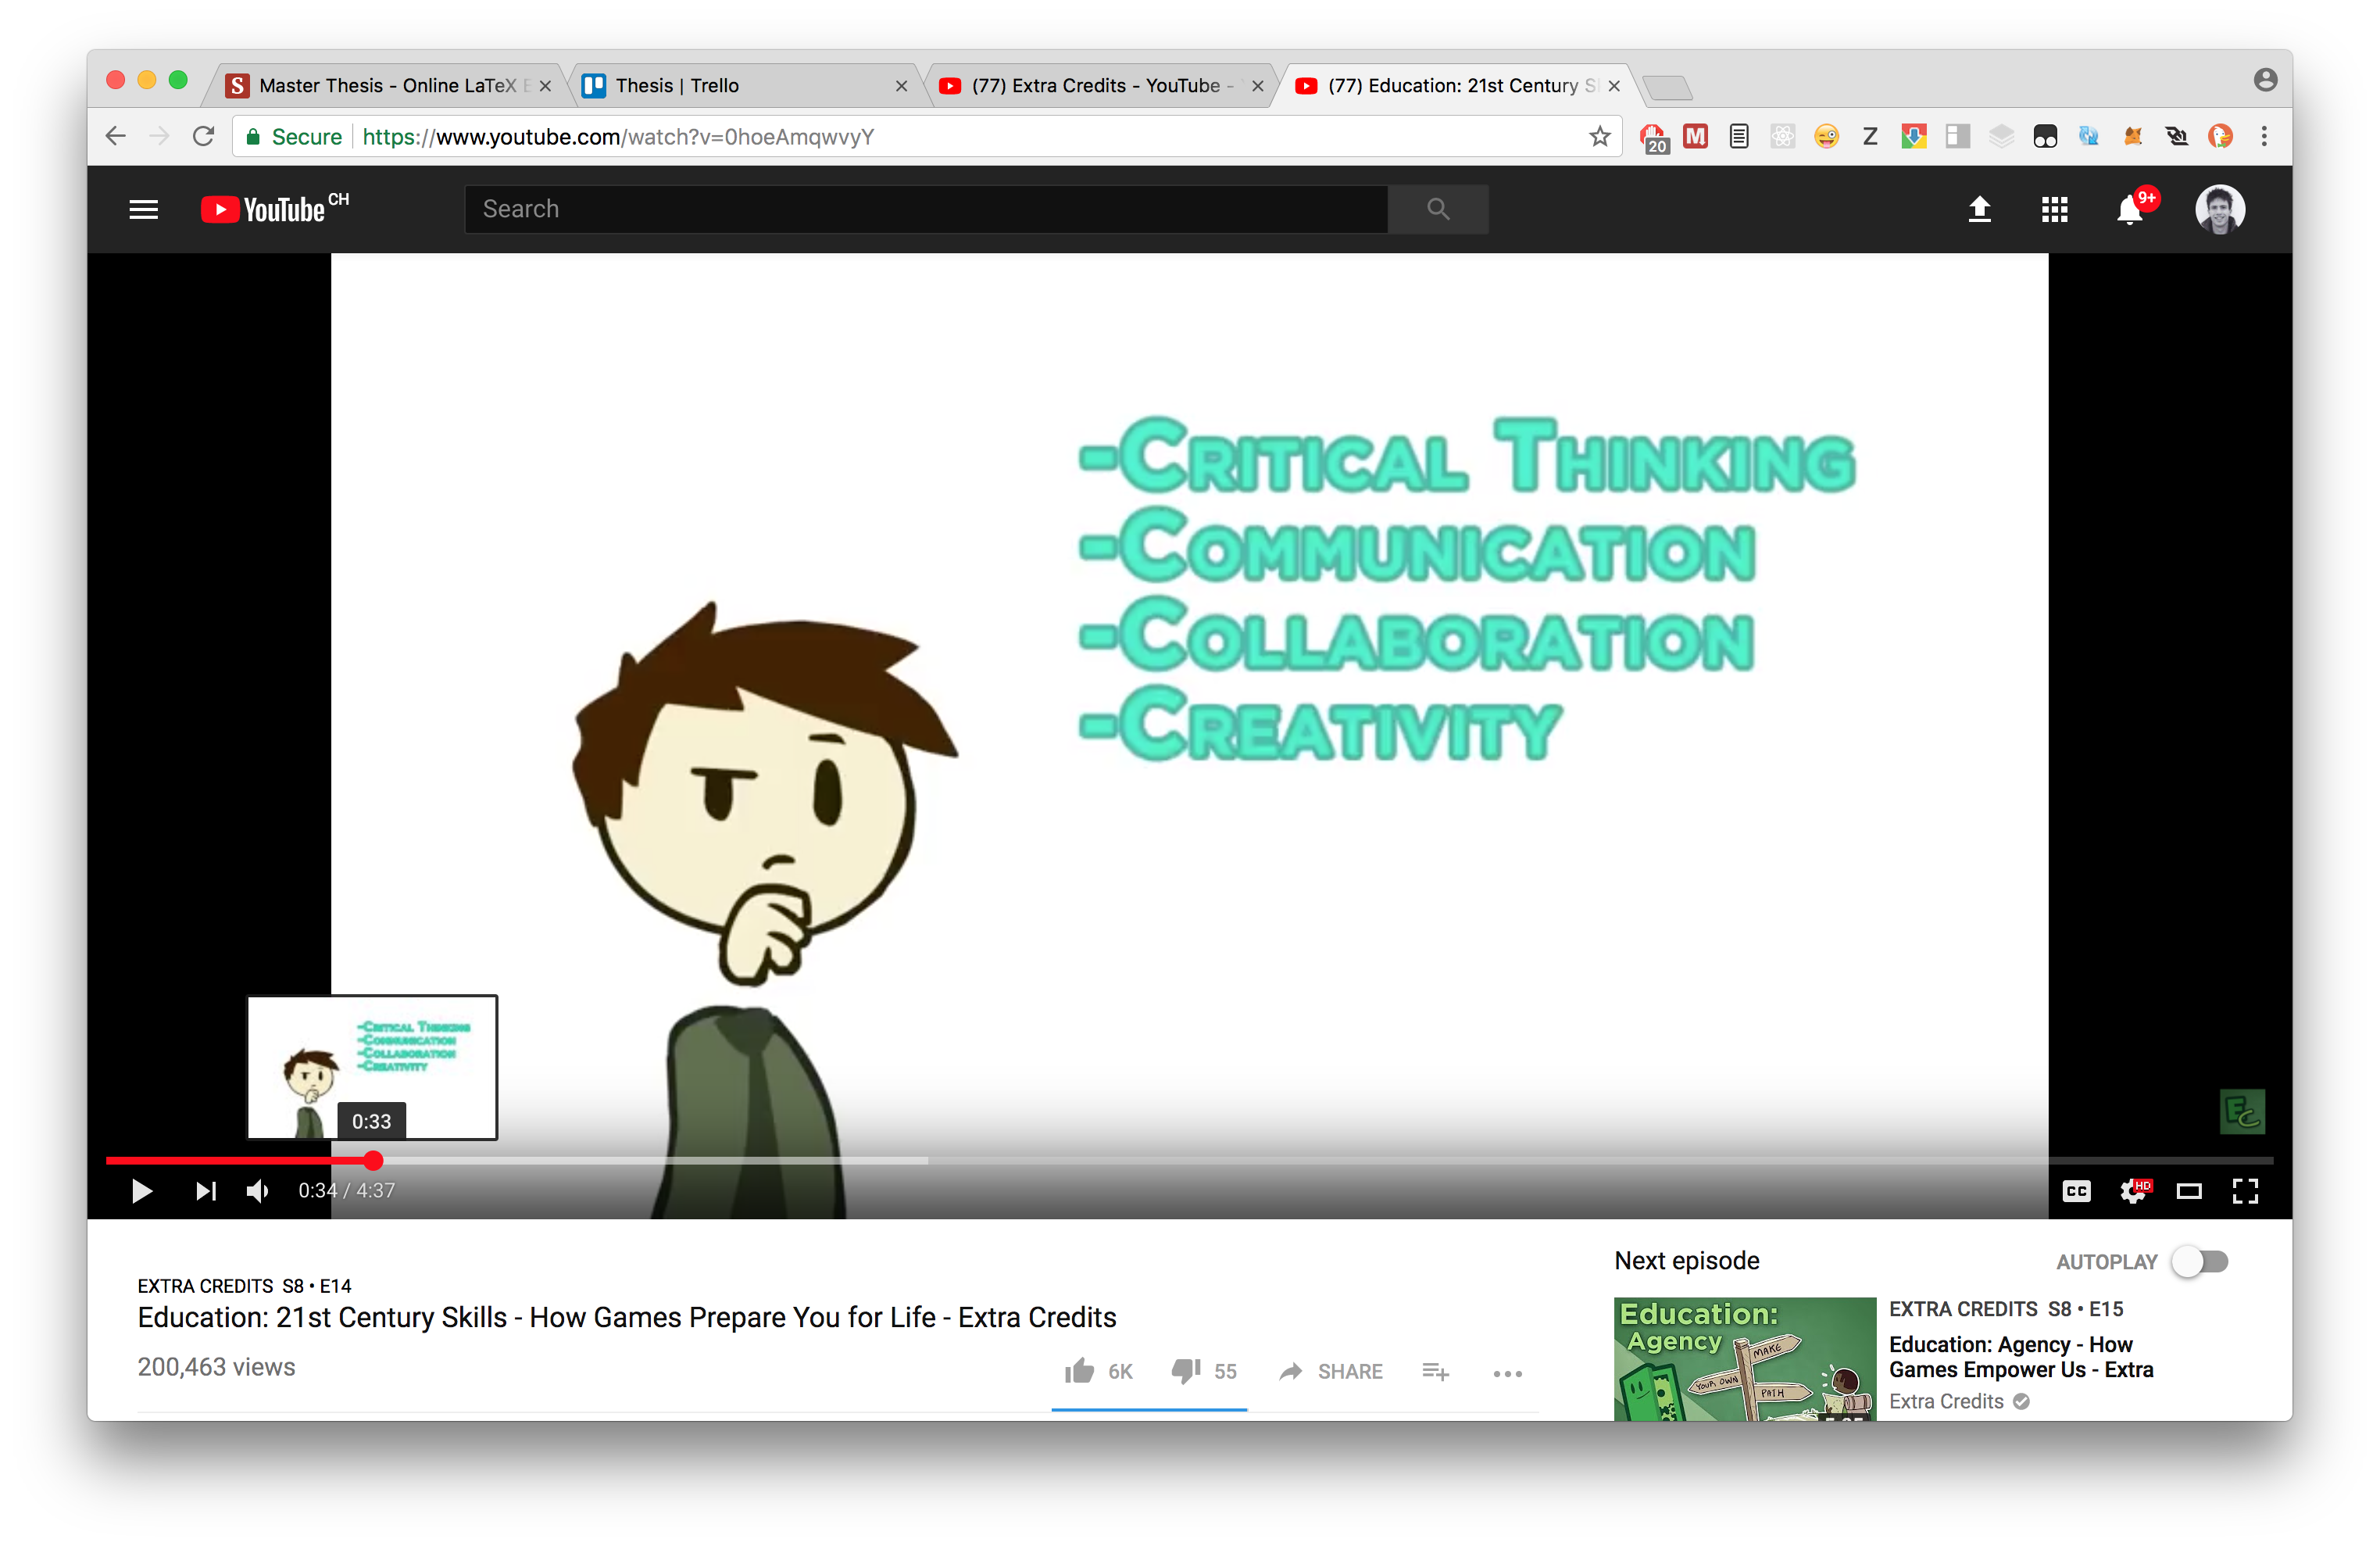
\includegraphics[width=1.35\textwidth, center]{time_scrubbing_mechanism.png} % quotation marks make sure file name does not display
\caption{An example of time scrubbing with a YouTube video. The red line could be dragged by the mouse to earlier or later times and resume playback there. The video itself is taken from a show called Extra Creditz, which talks about how game-design affects our lives for the better.}
\label{fig:normal_time_scrubbing}
\end{figure}

\section{Related work}
Before we start getting into the wonderland that is time scrubbing let us first look at related work in order to have some background knowledge. Some researchers also decided to present their work on YouTube which is arguably gives a much more intuitive introduction. The in-text citations of these papers are made \textbf{bold} (e.g. \textbf{[1337]}). When you, dear reader, look at the bibliography a YouTube URL will be there for you, so you can watch a demonstration of their work. Since we are going to look at time scrubbing systems it may be useful to first see systems in action rather than read academic articles.

Previous research on time scrubbing and related video browsing methods has mostly -- if not only -- been done for linear videos. In my own literature research I found that the biggest trend in time scrubbing research has been manipulating objects in video \cite{nguyen2013, shah2013, goldman2008, dragicevic2008, kimber2007}. The idea is that by manipulating an object within the video, a user is able to scrub along. 

Thumbnail like strategies are another way of doing this. For example, one study presented an interface in which a user sees still images of the video in a grid on their smartphone. When a user taps on one of these images, another set of still images are shown that are closer in time around the first tapped still image \cite{hi_story2012}. Another example is a study that used still images in a tree like fashion. The deeper levels presented still images for more fine-grained time scrubbing control whereas the levels closer to the root node were more coarse \cite{videotree2010}.

Then, there is a line of research that improves the experience of time scrubbing in some sort of fashion. For example, by implementing multiple time scrub bars \cite{multipletimeline1999}, altering the time scrubbing experience \cite{dynamictime2010}, by having automatic labels above or below the time scrub bar \cite{automaticsection2015} or manual ones\footnote{The custom-made video player of the Harvard course CS50: Introduction to Computer Science does this.} or by altering fast-forwarding functionality \cite{fastforward2009}.

Specifically for our interest, time scrubbing or related video browsing techniques have been developed purely for education and MOOCs. In one study, researchers improved the time scrub bar by looking at user statistics. Sections on the scrub bar where it has been stopped at or played at most were highlighted and when a user went over it with the mouse cursor it felt a bit resistant to continue to a non-highlighted part. It furthermore offers a search bar to search text in the transcript, which is mapped to the time it was said in the video. Finally, the most watched parts of the lecture have been automatically summarized. \cite{kim2014}. In another study, researchers created a complete system meant for YouTube educational videos. They created a word cloud in which they utilized the x-axis (temporal ordering in the video), y-axis (temporal spread), font-size (prominence) and font-color (level of acoustic stress). They furthermore created a second word cloud that summarizes a part of the video. A third feature they have are video slides that show points of interest for the next and previous slides, they also have a time scrub bar, which indicates on some points the auditory stress on certain concepts \cite{yadav2015}.

%Review
More information on this topic can be found in the literature review of Schoeffmann, Hudelist and Huber \cite{schoeffmann2015}. The previous information has been found by conducting my own literature search. The literature survey of Schoeffmann et al. is more comprehensive. However, the work of the following authors is not included in the review \cite{shah2013, goldman2008, dragicevic2008, kimber2007, multipletimeline1999, automaticsection2015, fastforward2009, kim2014, yadav2015}. This means that some work of 2013 and 2014 that I cited is not included and all works that I cited before 2009 and the year 2015 are not included. 


%Conclusions
Most conclusions of the reviewers are relevant for our purposes with XIMPEL. The reviewers found that many of the video browsing tools ``try to follow metaphors from real life, such as film strips, multiple parallel, displays and simulated tape recorders.'' Also, ``many interfaces make use of the third dimension.'' Most important of all, ``it is also observable that many tools try to make navigation in videos more convenient by using concepts like sliders with rubber band effects, direct manipulation of objects and synchronized display of thumbnails.'' \cite{schoeffmann2015} It is important to note that these are all conclusions based on what researchers and developers create. The conclusions cannot necessarily be drawn for the user or user experience. As of now, it is still not known to what extent users are waiting for these type of improvements. 

% Biggest critique of the review is no user evaluation
The reviewers formulated their biggest critique related to it: many studies did not perform a user evaluation. This means that a lot of studies have been peer reviewed and published on the idea of: having a justification based on an intuition, looking for related work, designing an own system and -- in most but not all cases -- presenting a prototype. 

%theory of users: scrub bar and watching video
Moreover, my own observation from the literature review is that very few theories and conceptual ideas about user behavior have been formed. There is, however, one study that did look at user behavior and attempted to infer a simple model out of that behavior. The researchers noticed that users mainly use the time scrub bar or simply watch the video from beginning and forward skip in time by a little bit, mostly using the mouse, and possibly restart the video to find what they need. What they did not do was make an educated guess and immediately jump to a specific point in time \cite{cobarzan2014}. 

% Hypervideo 360º
Unrelated, but worth mentioning is that one study in the literature review called 360 degree viewable video by the term \textit{hypervideo} \cite{neng2010}. This may indicate that previous research on hypervideo between 1990 and 2009 is a bit forgotton and now everything that extends the idea of video could potentially be called hypervideo.

\section{Within subject time scrubbing in XIMPEL}
Without the parallel media player, time scrubbing in XIMPEL is a straightforward concept. The way one would scrub with YouTube can be copied and pasted to any media type in XIMPEL -- including text, images and audio. 



% A XIMPEL application in purely sequential mode can be modeled as a directed graph of subjects as $G = (V, E)$ for which $V$ is the collection of subjects and $E$ denotes the direction of a transition from one subject to the next. This graph can be a tree or a graph with cycles, jumping from one subject to the next and back to the previous subject (completing the cycle). 

% Do you have multiple YouTube videos that you can manipulate individually? Or should it be at the level of a subject?

\subsection{Time scrubbing: the difficulties introduced by the parallel player}
%scrubbing within a subject
However, combining time scrubbing with the parallel player makes it more complicated. Now, a subject has control over multiple media types playing at the same time. The first question that make this question complicated is: (idea 1) should the user be able to control time scrub bars of individual media items? (idea 2) Or should the user be able to manipulate a global time scrub bar that will slide all the media items at once? The next two figures show the distinction visually. The visual example is only with videos. It is left as an exercise to the reader to imagine this with mixed media types (see figure \ref{images:local_scrub_bars} and \ref{images:global_scrub_bar_only}). 

\begin{figure}
\centering

\includegraphics[width=1.35\textwidth, center]{images/local_scrub_bars.png} % quotation marks make sure file name does not display
\caption{An example of how local scrub bars look like. They are completely independent of each other, and it is unknown to each scrub bar that there are other scrub bars and at what time they are resuming playback. Image credit: thumbnails from the educational show Crash Course (on YouTube).}
\label{images:local_scrub_bars}
\end{figure}

\begin{figure}
\centering
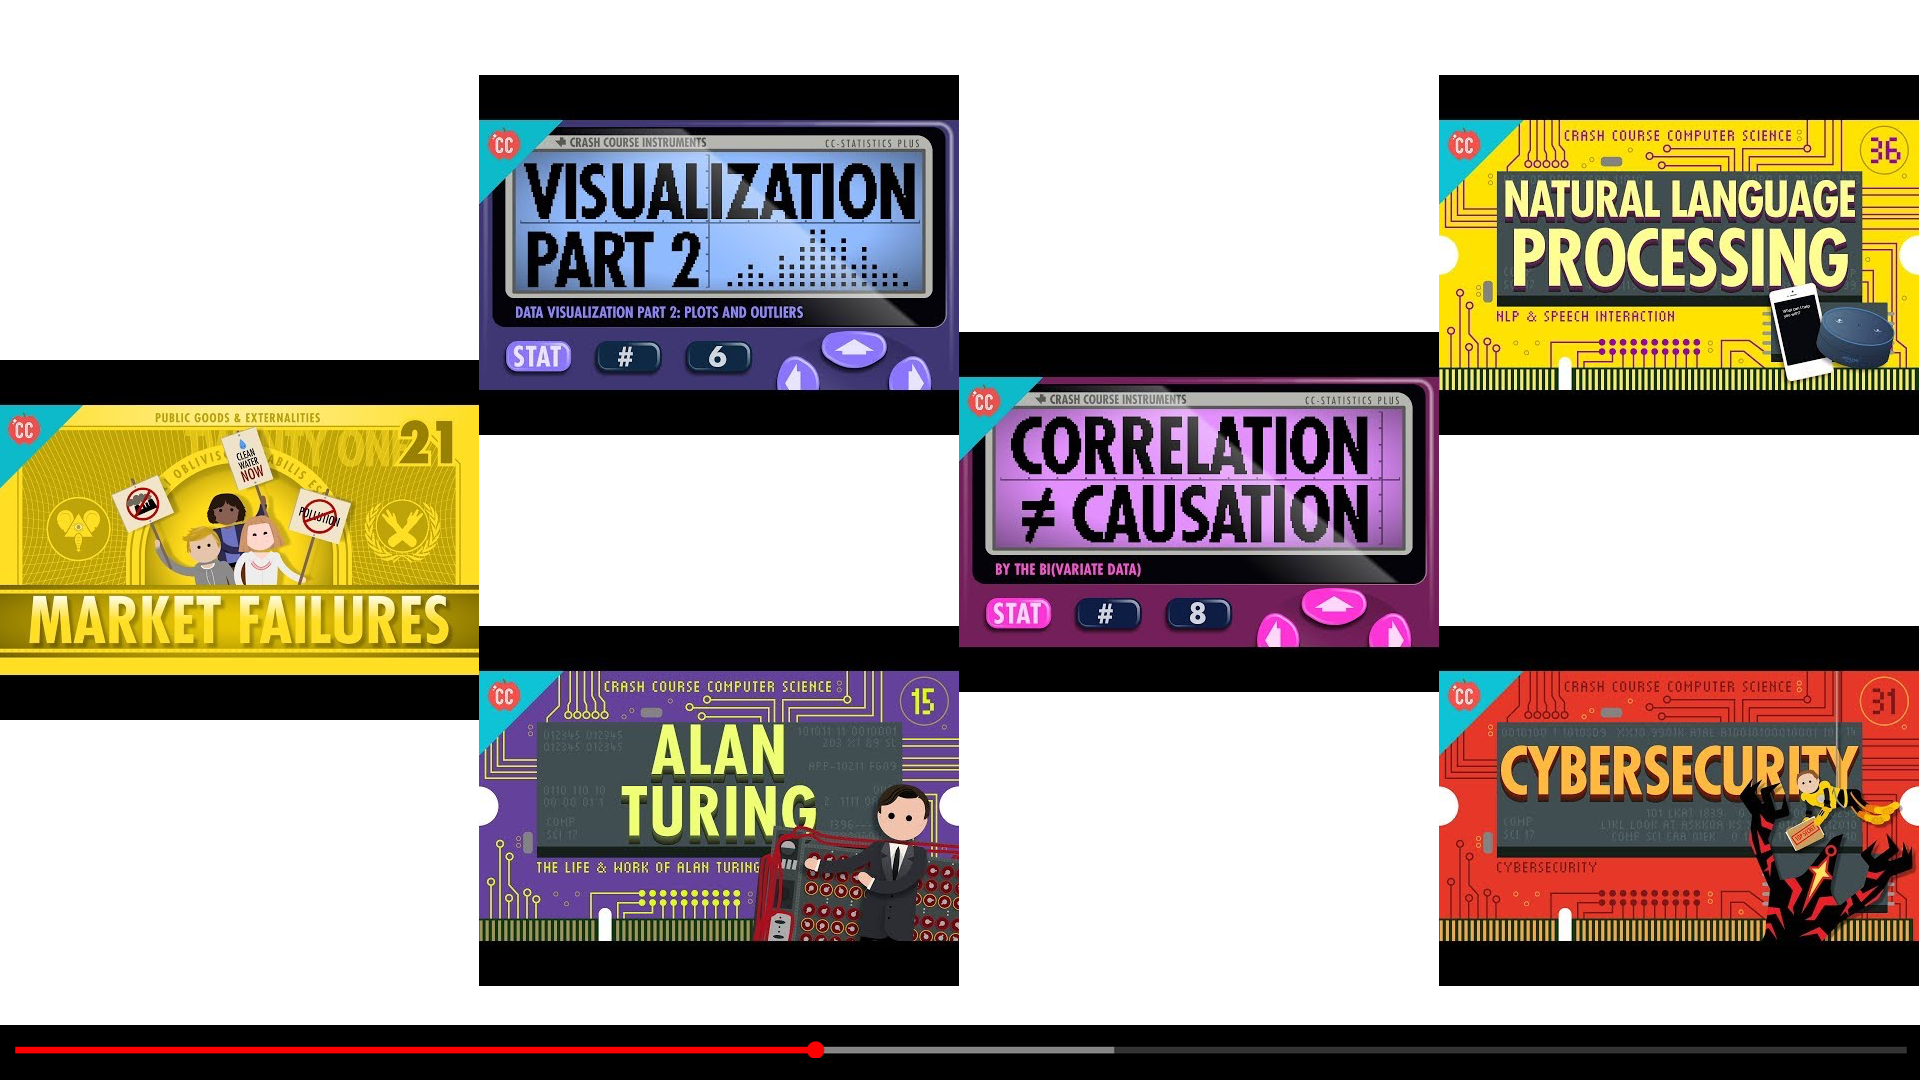
\includegraphics[width=1.35\textwidth, center]{images/global_scrub_bar_only.png} % quotation marks make sure file name does not display
\caption{An example of how a global scrub bar looks like. One scrub bar manipulates the time for all media items in the presentation. Image credit: thumbnails from the educational show Crash Course (on YouTube).}
\label{images:global_scrub_bar_only}
\end{figure}

Manipulating the individual time scrub bars is still fairly straightforward (idea 1 and figure \ref{images:local_scrub_bars}), since the interface does not change. The time scrub bar interface simply displayed more often in the XIMPEL application. The complicatedness, increases when one tries to answer the second question (idea 2 and figure \ref{images:global_scrub_bar_only}). It could be argued to choose for either ideas (1, the local multiple time scrub bars or 2, the global time scrub bar), both ideas need to have a conceptual realization.

\begin{figure}
\centering
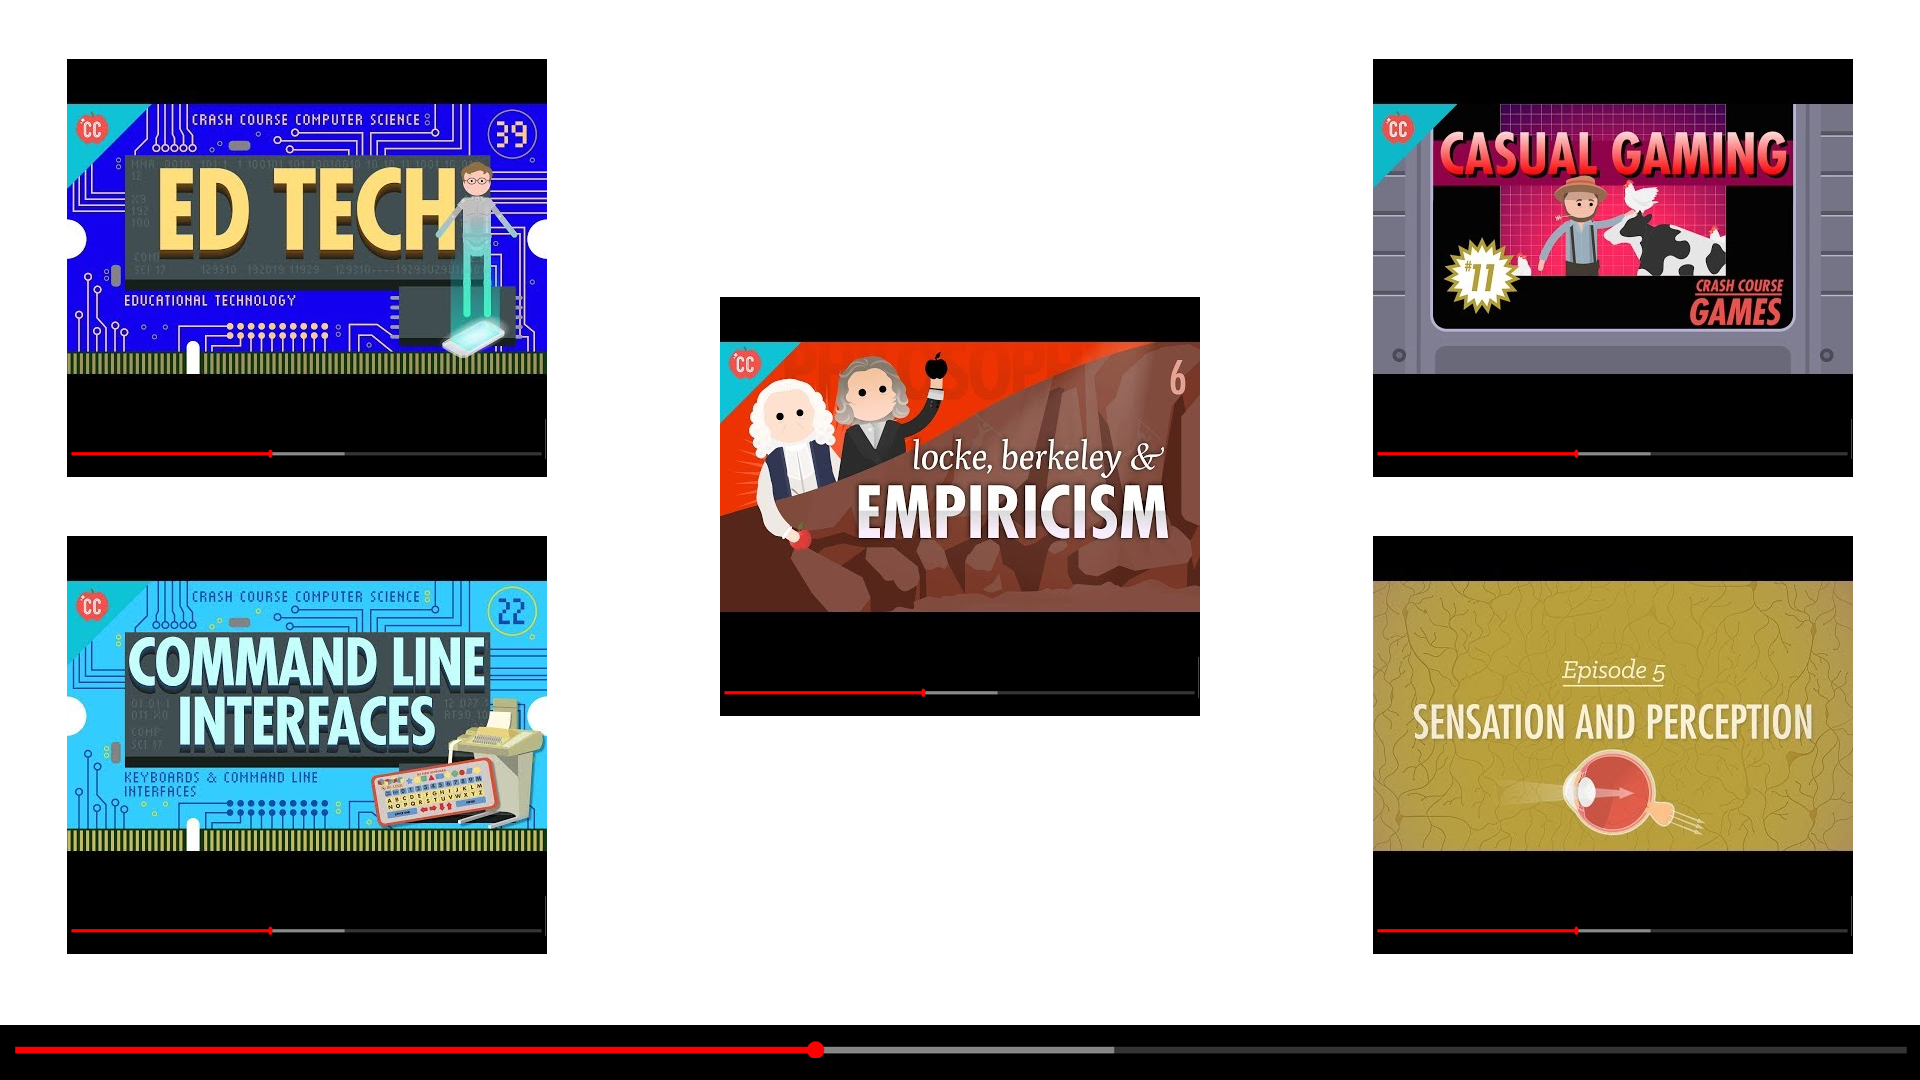
\includegraphics[width=1.35\textwidth, center]{images/global_scrub_bar_with_locals.png} % quotation marks make sure file name does not display
\caption{An example of how a global scrub bar looks like with local scrub bars. The global scrub bar manipulates the time of the local scrub bars but the local scrub bars can also be manipulated individually. Image credit: thumbnails from the educational show Crash Course (on YouTube).}
\label{images:global_scrub_bar_with_locals}
\end{figure}

% For now, let us focus on idea 2: how does one create a global time scrub bar in XIMPEL? The first straightforward solution (concept 2a) would be to have a global scrub bar mapped to individual scrub bars of each media type. This concept would marry idea 1 and 2 by having local time scrub bars and local time scrub bars.

%marrying local and global scrub bar
Moreover, idea 1 and 2 could be combined together by having a global scrub bar and local scrub bars (see figure \ref{images:global_scrub_bar_with_locals}). However, user studies would need to be done in order to validate the concept. Most web applications do not have multiple scrub bars, and therefore it might be a bit too overwhelming for the user.

% \begin{figure}
% \centering
% 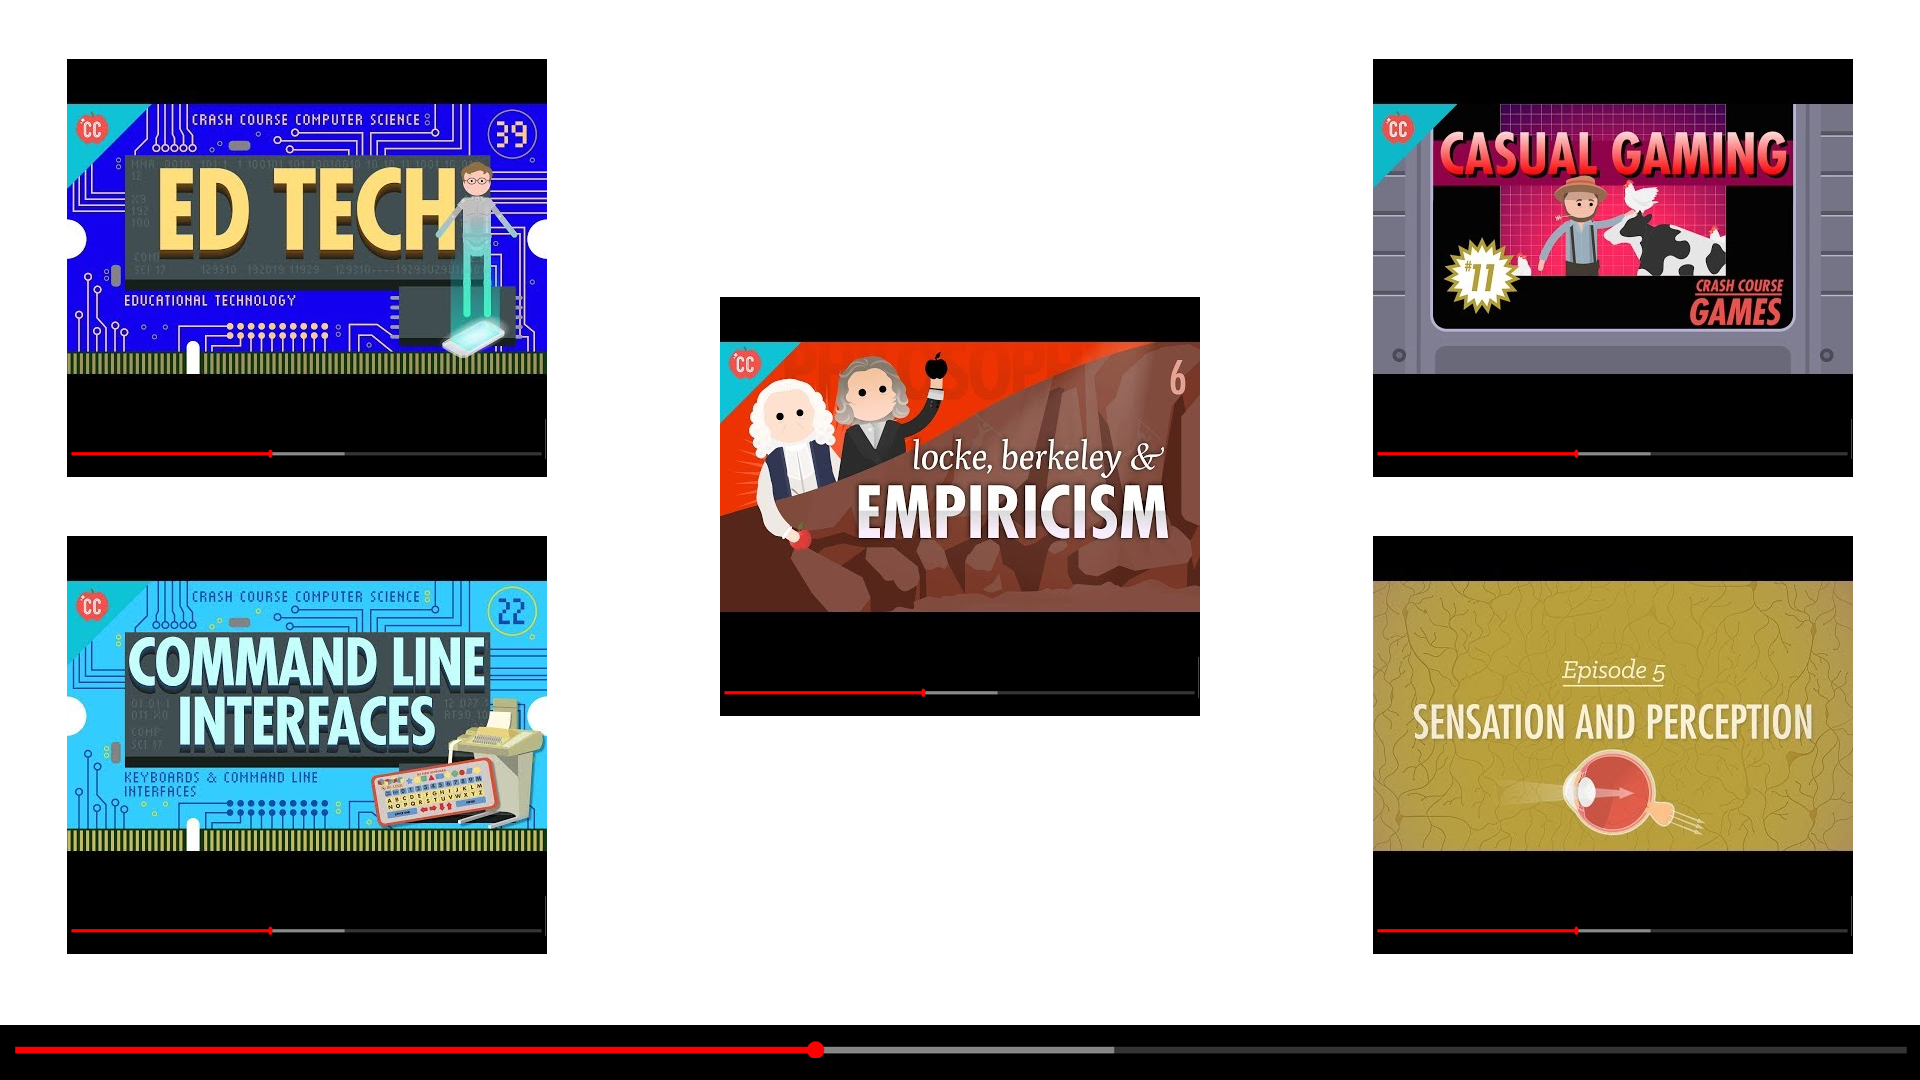
\includegraphics[width=1.35\textwidth, center]{images/global_scrub_bar_with_locals.png} % quotation marks make sure file name does not display
% \caption{An example of how a global scrub bar looks like with local scrub bars. The global scrub bar manipulates the time of the local scrub bars but the local scrub bars can also be manipulated individually. Image credit: thumbnails from the educational show Crash Course (on YouTube).}
% \label{images:global_scrub_bar_with_locals}
% \end{figure}


%talk about limitations of marrying ideas
The limitation of marrying these ideas is that when you time scrub the global one a design decision needs to be taken. If a user already scrubbed one time scrub bar locally and then scrubs globally, three different scrubbing situations could occur (see figure \ref{images:move_along_with_global}, \ref{images:move_along_with_offset} and \ref{images:catch_up}). Either the global time scrub bar resets the local time scrub bar to the original mapping where the global time scrub bar believes it to be. For example, a global time scrub bar is at 50\%, so all the local time scrub bars will be reset to 50\%. Another possibility is that local time scrub bars that have been meddled with, will move along according to the offset of the global time scrub bar. For example, the global time scrub bar is scrubbed from 30\% to 50\%, representing a 20\% increase. One local scrub bar has been scrubbed to 75\% prior. Then, it will increase to 95\% and the other local scrub bars, that have not been meddled with, will move to 50\%. The final possibility is that the meddled local scrub bars do not move if they are ahead of the global scrub bar, and will catch up and reset to the value of the global scrub bar when they are behind. Again figure \ref{images:move_along_with_global}, \ref{images:move_along_with_offset} and \ref{images:catch_up} visually clarify these difficulties.



% Three possibilities:
% 1. move along with scrub bar
% 2. move along with offset
% 3. catch up mechanic and otherwise do what you want

\begin{figure}
\centering
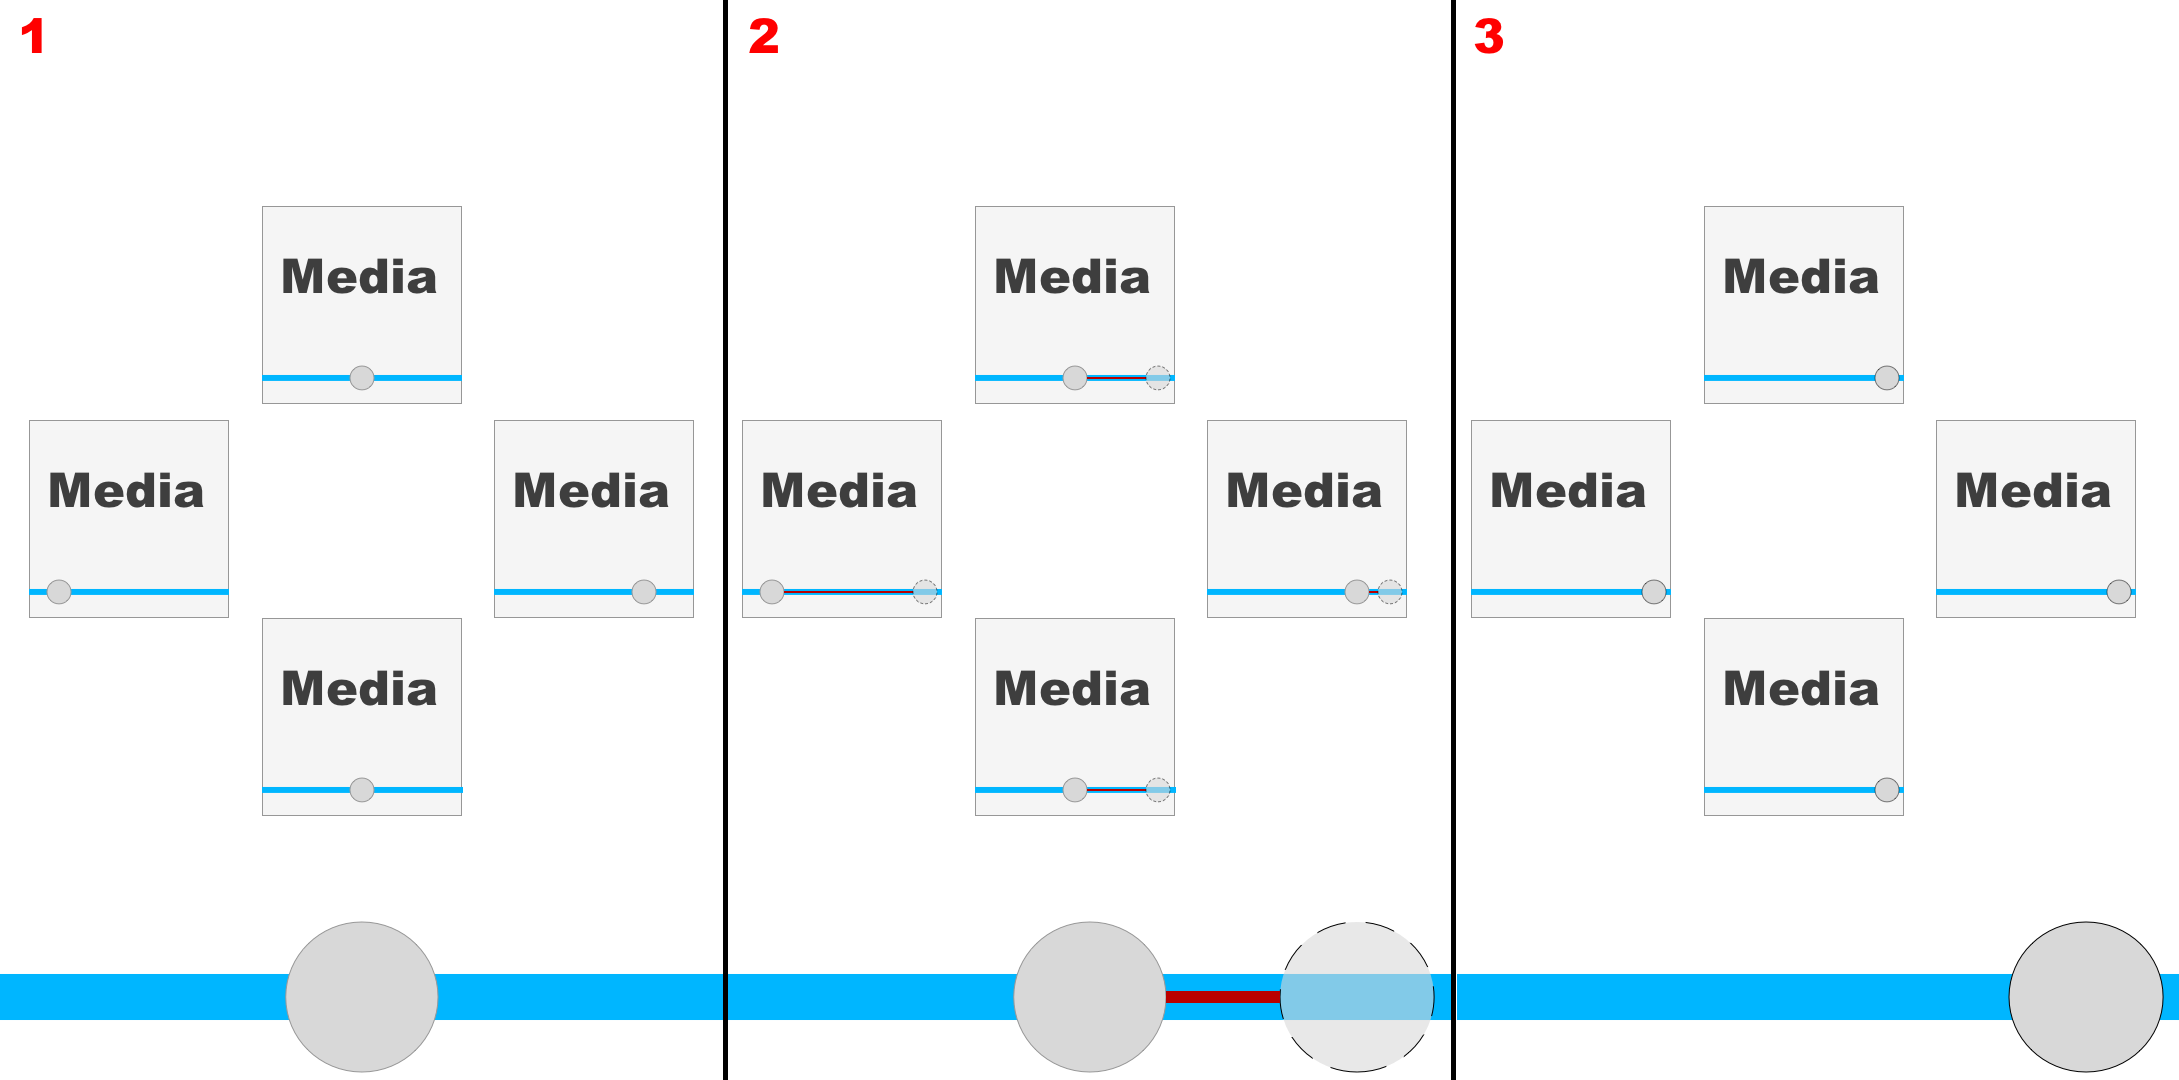
\includegraphics[width=1.35\textwidth, center]{images/move_along_with_global.png} % quotation marks make sure file name does not display
\caption{The global time scrub bar determines where all local scrub bars will resume playback.}
\label{images:move_along_with_global}
\end{figure}

\begin{figure}
\centering
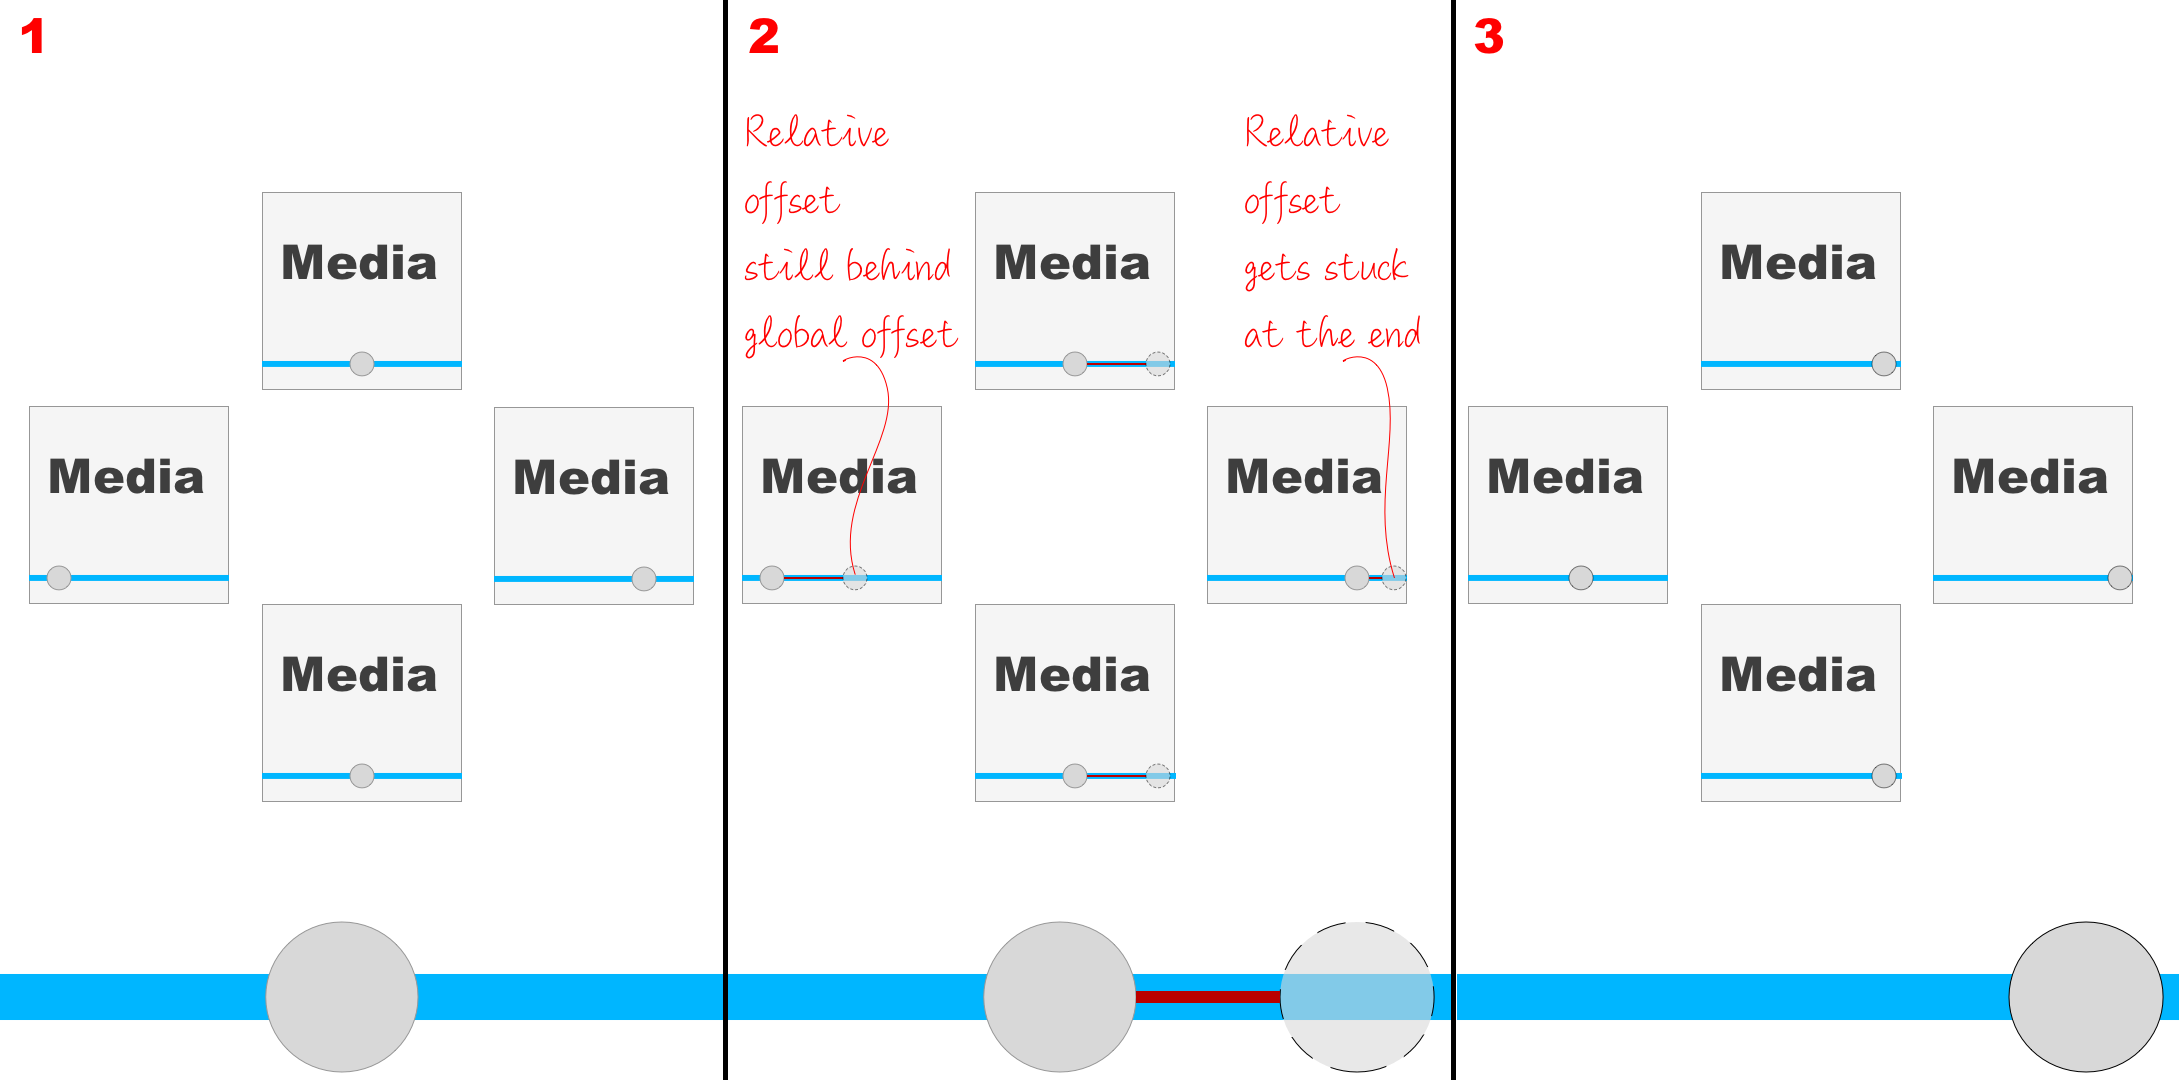
\includegraphics[width=1.35\textwidth, center]{images/move_along_with_offset.png} % quotation marks make sure file name does not display
\caption{The global time scrub bar determines the percentage offset that local scrub bars will give to their position in time.}
\label{images:move_along_with_offset}
\end{figure}

\begin{figure}
\centering
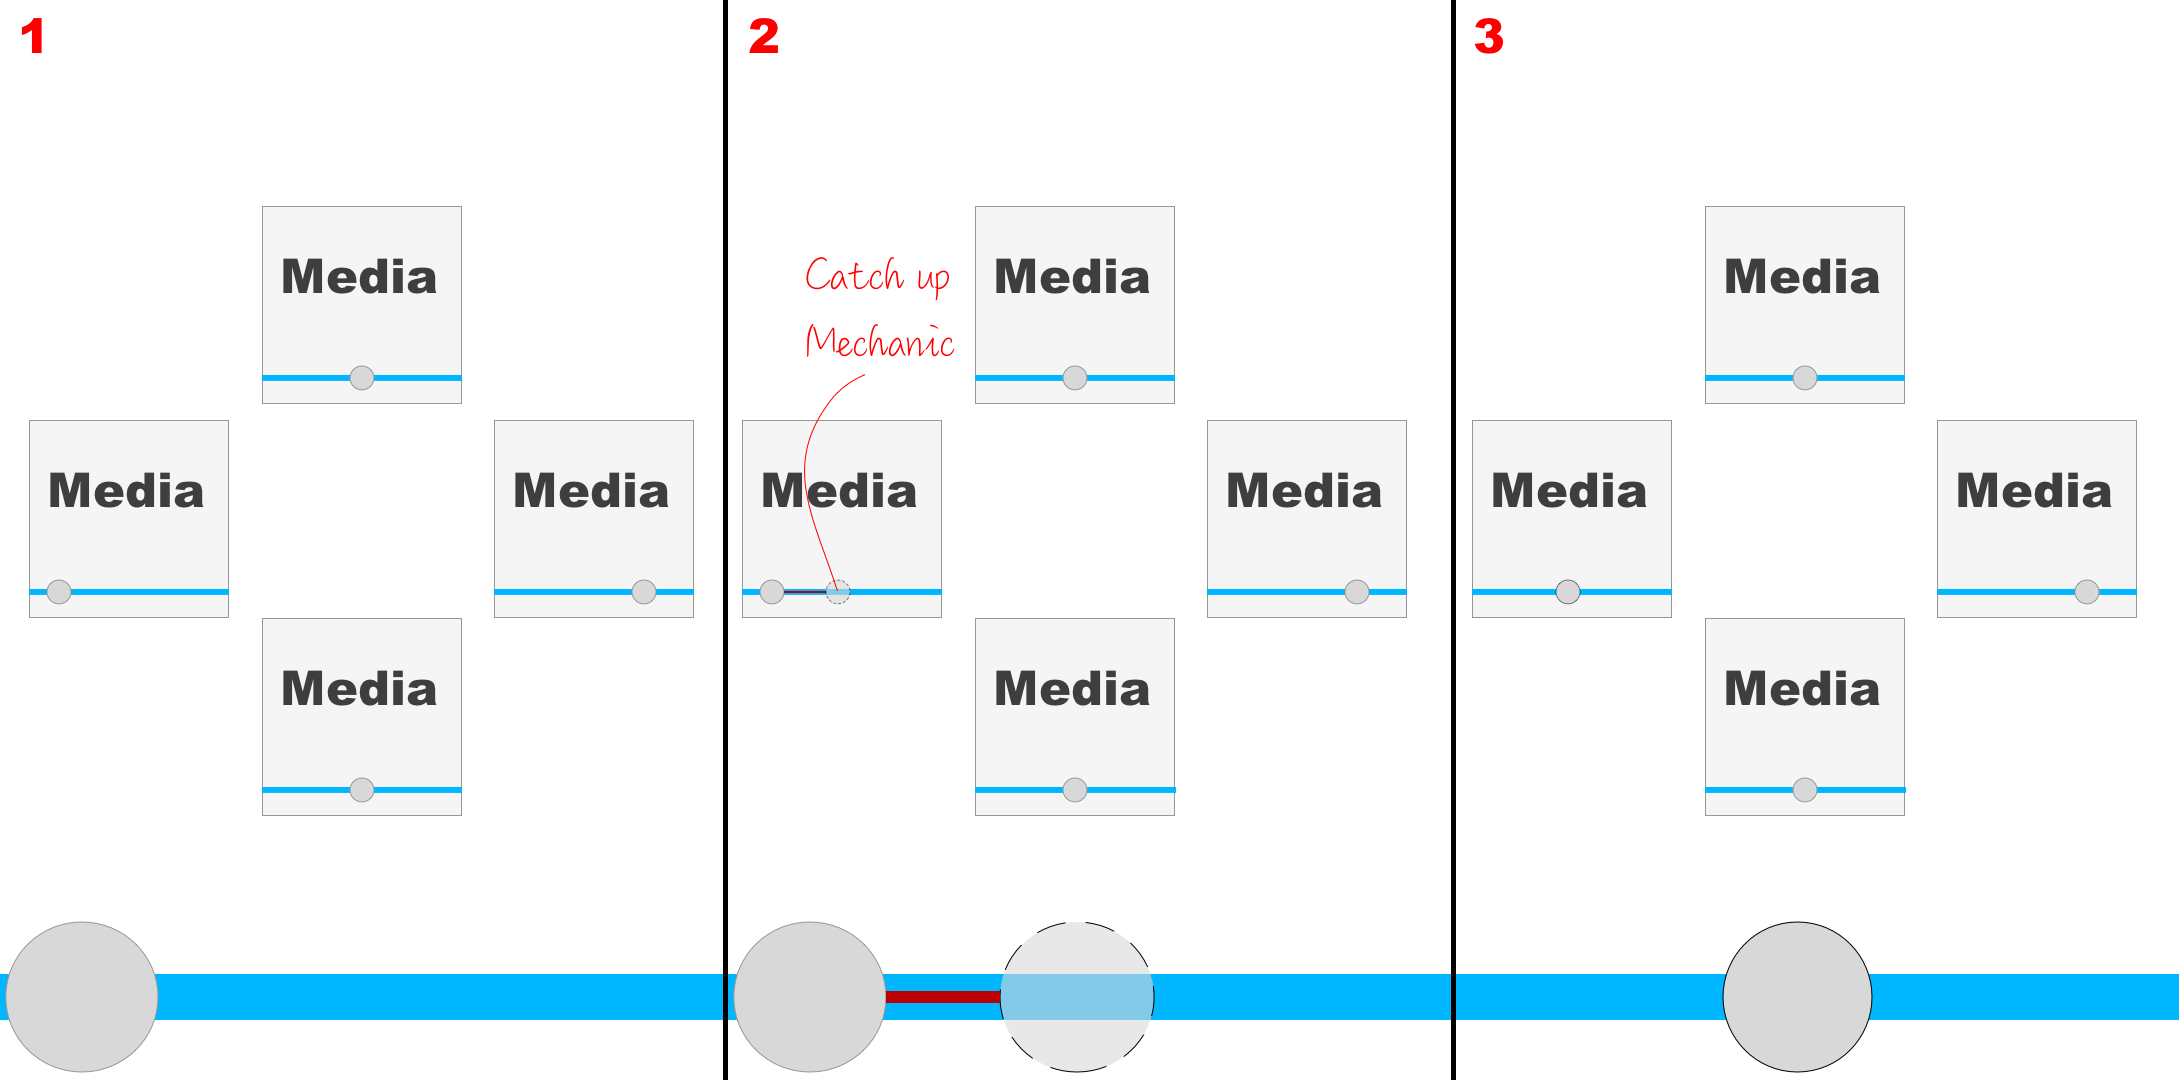
\includegraphics[width=1.35\textwidth, center]{images/catch_up.png} % quotation marks make sure file name does not display
\caption{The local scrub bars catch up with the global time scrub bar, but only if the local scrub bars are behind the global time scrub bar. There is also an inverse situation possible, here the local scrub bars will catch up to the global time scrub bar if they are ahead. This inverse situation is not shown in the figure. In the figure only one media item needs to catch up with its local scrub bar.}
\label{images:catch_up}
\end{figure}


\subsection{Time scrubbing: the difficulties introduced by users having choice}
The real difficulty is introduced not by the parallel player but by XIMPEL and the nature of interactive video and choice itself. One could ask herself or himself: if one scrubs from 30\% to 50\% but on the 40th percentile of the time line an overlay should be presented with a choice, should that choice be known to the user or not? The user may not know that there would be an overlay on the 40th percentile and therefore may not be aware of the choice. The user may also be specifically skipping to the 50th percentile, because the user knows there is an overlay there and wants to skip it.

In a single YouTube video this is less of an issue. YouTube overlays tend to be links to different videos that are less coherent compared to a certain group of hypermedia applications in XIMPEL. The user experience (UX) designers of YouTube presumably have decided that it is okay to skip these overlays. But should the user experience of XIMPEL be similar?

Both UX proposals would need to be tested. And while it is easy to copy the UX of YouTube, it is a less easy question to create a new UX in the case that overlays should be presented to a time scrubbing user. In order to answer this question I am forced to take inspiration from other systems or create something of my own and justify it.

Furthermore, is it desirable in XIMPEL presentations to inform the user that he or she is skipping overlays? Or is it more desirable to inform the user it is skipping a moment of choice. In the first scenario all overlays would need to be known by the user in advance. In the second scenario the user only needs to know whether there is any overlay present at certain moments in time, it does not matter how many overlays there are.

For this question, I take inspiration from the time scrubbing mechanism that professor David J. Malan and his colleagues have developed for the course CS50 at Harvard. The reason for that is because it solves a similar problem and it was usable for me when I took the course years ago. The problem that they solved is that during a lecture a student would be introduced to multiple topics or sub-topics. Since the level difference between the students is quite big, some students may want to skip certain topic. By creating a time scrub bar that allows students to knowingly skip a certain lecture topic, they give the power (the choice) to students to do so. In other words, their problem is also a problem about choice, albeit a different form of choice. 

% TO DO: You left at the CS50 interface.

Figure \ref{images:cs50_player} will show the user interface design. Like CS50 we highlight certain points of the time scrub bar. By doing this, the user is able to know when there will be a potential choice. When the user hovers over such a point, the user will see all possible choices that he or she can make at such a point. This interface is relevant for people who already went through a XIMPEL presentation. In some cases, the XIMPEL author may want to disable this feature since not knowing when certain decisions ought to be made potentially add value to the UX of a XIMPEL application.

This interface works well for one media item? Would such an interface scale for multiple media items? For that dear reader I ask you to use your imagination. Imagine multiple media items, for example, two videos, one audio and one image somewhere on the screen. Got it? Amazing! When all media items have their own time scrub bar -- or in the case of the image at least a time line which you cannot interact with -- then highlighting certain points on the time scrub bar or time line is not an issue. In this way it does scale. However, it is also possible to put all the highlighted points at a global time scrub bar. The possible disadvantaged is that a user cannot identify to which media item the choice belongs to, which is a piece of information that may or may not be important depending on the XIMPEL presentation being played.

\begin{figure}
\centering
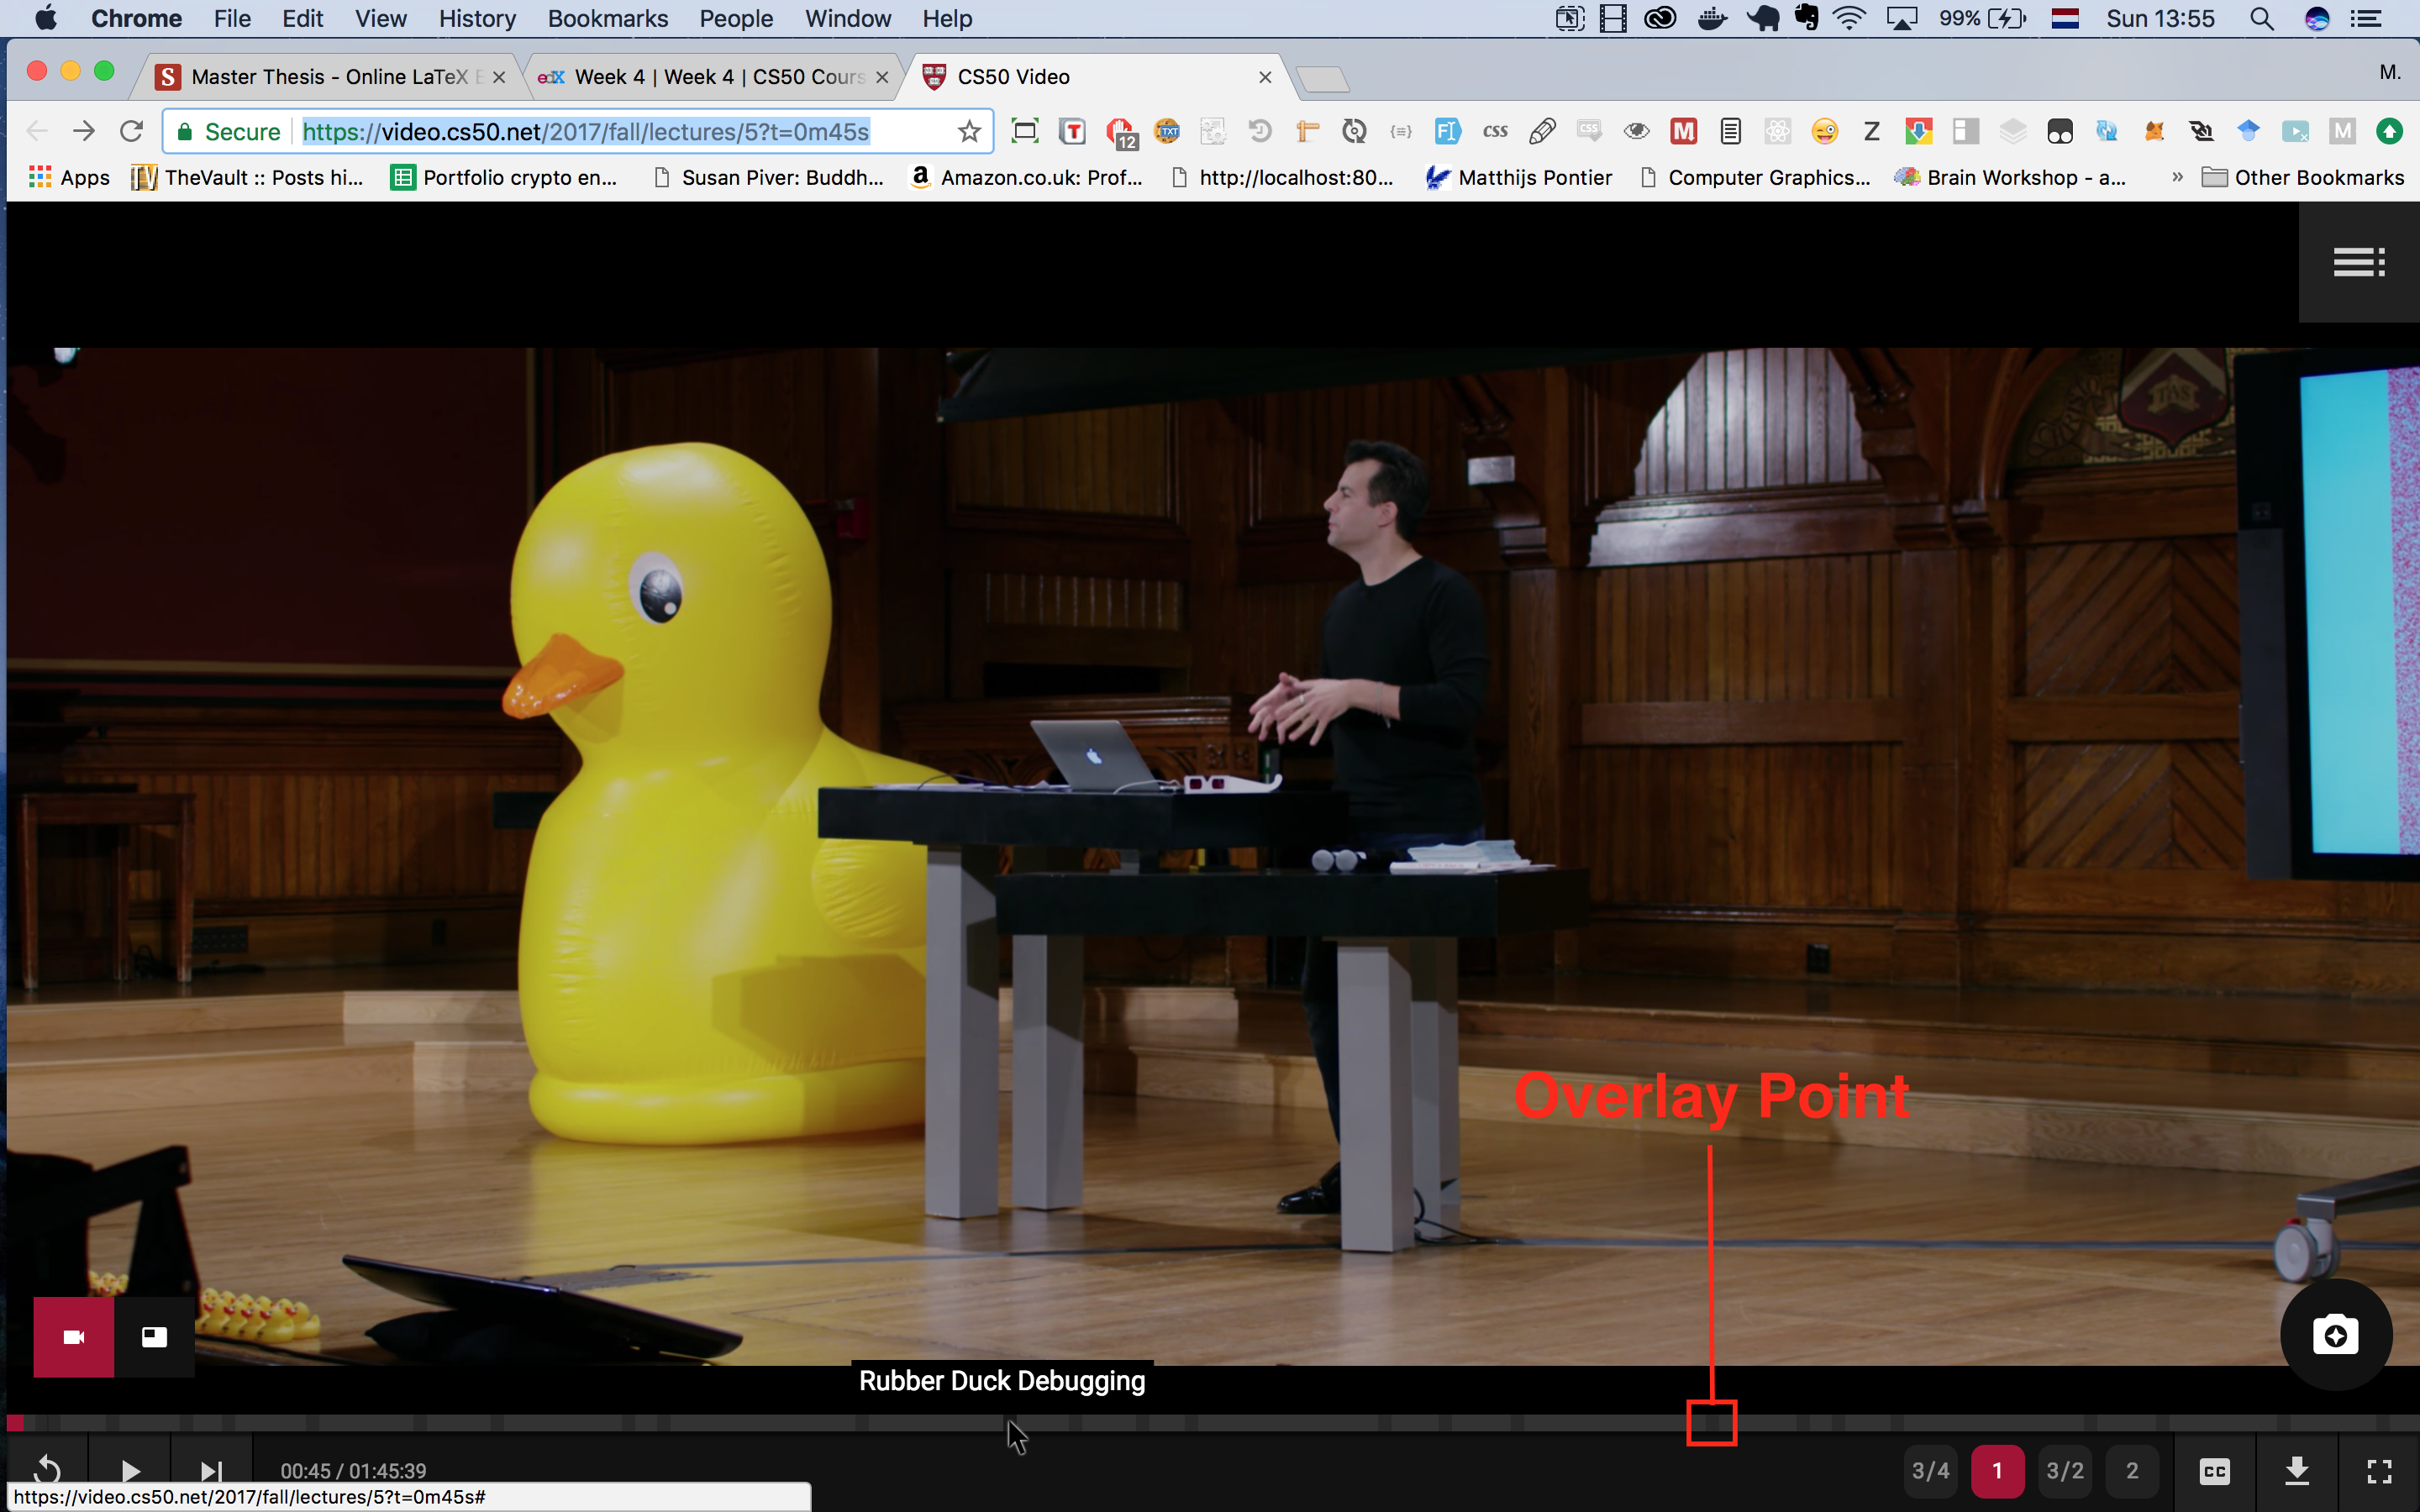
\includegraphics[width=1.35\textwidth, center]{images/cs50_player.png} % quotation marks make sure file name does not display
\caption{An example of the CS50 player. In this screenshot the mouse hovered over an overlay point called Rubber Duck Debugging.}
\label{images:cs50_player}
\end{figure}

\section{Between subject time scrubbing in XIMPEL}
Now that I have outlined which possible design dilemma's by having choice within XIMPEL and the newly built parallel player introduces within a subject, let us look what interactive video or rather XIMPEL itself introduces. What if we do not want to time scrub within a subject but between subjects? From a user experience point of view this is entirely possible because users may experience the interactive video as a whole, and perhaps they would want to skip certain scenes, or maybe skip halfway.

It is important to understand that this is a wicked problem, meaning: ``a problem with multiple plausible solutions as well as multiple subjective interpretations of such solutions. \cite{olsson2014}'' The paper of Carl Magnus Olsson, Staffan Björk and Steve Dahlskog goes into detail about what wicked problems are, how it relates to design (and game-design in particular) and how to deal with them \cite{olsson2014}. For now, it suffices to understand what a wicked problem is, in our case devizing solutions really means making compromises between ease of use and having more information. I will present two different designs which emphasizes one or the other. In order to see which design would be better, user studies would need to be conducted for which I unfortunately lack the time.

% 1: show full graph
We could show more information by having a screen that displays the full interaction graph of XIMPEL. The user would be able to see at exactly which point a choice would be made and would be able to scrub along the time graph (it is not a time line anymore) and land at the point where he or she wants to be. The issue with this is that this may, in some cases, neglect the idea of interactive video. By giving a user the possibility of seeing the interaction points, the author of a XIMPEL application would be forced to give away a part of the surprise. An example of such a graph is shown in figure \ref{tikz:full_graph}.

% For scaling see: https://tex.stackexchange.com/questions/4338/correctly-scaling-a-tikzpicture
% For captioning it see: https://tex.stackexchange.com/questions/28258/what-is-the-correct-way-to-caption-a-tikzpicture
% The picture: is tested at: https://www.sharelatex.com/project/5ab8f520af30be4134f56286
\begin{figure}
\centering
\scalebox{0.5}{
\begin{tikzpicture} %[scale=0.5]
\begin{scope}[every node/.style={circle,thick,draw, align=center}]

    %Subject: De Bonte Hen 
    \node (MenuDeBonteHen) at (0,0) {Menu\\De Bonte Hen};
    \node (WalkToHetJongeSchaap) at (5,5) {Walk to\\Het Jonge Schaap};
    
    \node (QuizBonteHenIntro) at (5,0) {Quiz\\De Bonte Hen intro};
    \node (QuizMenuDeBonteHen) at (10,0) {Quiz Menu\\De Bonte Hen};
    \node (WrongBonteHenQuiz) at (15,5) {Wrong answer};
    \node (CorrectBonteHenQuiz) at (15,-5) {Right answer};
    \node (CorrectBonteHenQuizInfo) at (20,-5) {Correct answer information};
    
    \node (TourOfMolenDeBonteHen) at (5,-5) {Tour of windmill\\De Bonte Hen};
    
    %Subject: Het Jonge Schaap 
    \node (MenuMolenHetJongeSchaap) at (10,15) {Menu\\Molen Het Jonge Schaap};
    \node (MenuDeZoeker) at (15,21) {Menu\\De Zoeker};
    
    \node (QuizJongeSchaapIntro) at (15,15) {Quiz\\Het Jonge Schaap};
    \node (QuizJongeSchaapMenu) at (20,15) {Quiz\\Het Jonge Schaap};
    \node (WrongJongeSchaapQuiz) at (25,20) {Wrong answer};
    \node (CorrectJongeSchaapQuiz) at (25,10) {Right answer};
    \node (CorrectAnswerJongeSchaapInfo) at (30,10) {Correct answer information};
    
    \node (TourOfMolenHetJongeSchaap) at (15,10) {Tour of\\Molen Het Jonge Schaap};
    
    %Subject: De Zoeker
    \node (DeZoeker) at (20,21) {De Zoeker\\(subtree truncated)};
    
\end{scope}

\begin{scope}[>={Stealth[black]},
            %   every node/.style={fill=white,circle},
              every edge/.style={draw=red,very thick}]
              
    %Subject: De Bonte Hen
    \path [->] (MenuDeBonteHen) edge node {} (WalkToHetJongeSchaap);
    \path [->] (MenuDeBonteHen) edge node {} (QuizBonteHenIntro);
    \path [->] (MenuDeBonteHen) edge[bend left=5] node {} (TourOfMolenDeBonteHen);
    
    \path [->] (TourOfMolenDeBonteHen) edge[bend left=5] node {} (MenuDeBonteHen);
    
    \path [->] (QuizBonteHenIntro) edge node {} (QuizMenuDeBonteHen);
    \path [->] (QuizMenuDeBonteHen) edge node {} (WrongBonteHenQuiz);
    \path [->] (WrongBonteHenQuiz) edge[bend right=10] node {} (MenuDeBonteHen);
    \path [->] (QuizMenuDeBonteHen) edge node {} (CorrectBonteHenQuiz);
    \path [->] (CorrectBonteHenQuiz) edge node {} (CorrectBonteHenQuizInfo);
    \path [->] (CorrectBonteHenQuizInfo) edge[bend left=60] node {} (MenuDeBonteHen);
    
    %Subject: Het Jonge Schaap
    \path [->] (WalkToHetJongeSchaap) edge node {} (MenuMolenHetJongeSchaap); %Transition
    
    \path [->] (MenuMolenHetJongeSchaap) edge node {} (MenuDeZoeker);
    \path [->] (MenuMolenHetJongeSchaap) edge node {} (QuizJongeSchaapIntro);
    \path [->] (MenuMolenHetJongeSchaap) edge[bend left=5] node {} (TourOfMolenHetJongeSchaap);
    
    \path [->] (TourOfMolenHetJongeSchaap) edge[bend left=5] node {} (MenuMolenHetJongeSchaap);
    
    \path [->] (QuizJongeSchaapIntro) edge node {} (QuizJongeSchaapMenu);
    \path [->] (QuizJongeSchaapMenu) edge node {} (WrongJongeSchaapQuiz);
    \path [->] (WrongJongeSchaapQuiz) edge[bend right=5] node {} (MenuMolenHetJongeSchaap);
    \path [->] (QuizJongeSchaapMenu) edge node {} (CorrectJongeSchaapQuiz);
    \path [->] (CorrectJongeSchaapQuiz) edge node {} (CorrectAnswerJongeSchaapInfo);
    \path [->] (CorrectAnswerJongeSchaapInfo) edge[bend left=65] node {} (MenuMolenHetJongeSchaap);
    
    %Subject: De zoeker
    \path [->] (MenuDeZoeker) edge node {} (DeZoeker);
    
\end{scope}
\end{tikzpicture}
}
\caption{In this figure a part of full interaction graph of the XIMPEL presentation of the Zaanse Schaans is shown. Users who would like to scrub between subject could see a graph like this, and click on any part of the edge to indicate how far they want to start in a subject. A graph like this could be shown in the upper right corner by clicking on a button, for example. What is not shown in this image is that overlays could be displayed on any part of the edge as well for additional scrubbing information.}
\label{tikz:full_graph}
\end{figure}


In normal time scrubbing this is not a problem. Consider a horror movie -- where there are a lot of surprises. When a person scrubs further along the time line, he or she has no idea what to expect. This is because nothing is highlighted other than the time. With showing the full interaction graph it may not only be needed to show where the interaction points are, but also which interaction points. Whether users prefer a full interaction graph with only nodes and edges going out of nodes or also see labeled possible interactions on the nodes would require user testing. 

% 2: show a simple way to skip scenes with overlays as is possible within current XIMPEL
The simpler way of doing time scrubbing in XIMPEL is creating a scene skipping feature. With the current capabilities of XIMPEL this is already possible. It is even possible to show all possible options for the next scene as an overlay that the user could click or tap on. While it is a crude way of time scrubbing, it is an easier interface and perhaps therefore more usable. An example of this is done in the Zaanse Schans XIMPEL presentation (see \url{http://classic.ximpelapps.nl/zaanseschans_html5}).

\section{Interaction of within and between subject time scrubbing}
% D. 50% of 5th subject --> leave state in a certain way --> what if user scrubs bag to it?
When a user scrubs within a subject, as soon as the user moves to scrub time between subjects it begs the question whether a XIMPEL application should remember the scrubbed state within the subject or whether it should not. If it should, then the concept of time becomes slightly different. For example, a user scrubs the 50th percentile of the fifth subject with the between subject scrubber, then if the user left the state of that subject in a certain way it needs to be recalculated what it means to scrub to the 50th percentile of it with respect to the offset of where the user left it. Imagine a user clicking on the middle of the upper arrow between \textit{Menu De Bonte Hen} and \textit{Tour of windmill De Bonte Hen} in figure \ref{tikz:full_graph} (lets call this user action A). Then the user would be transported to the middle of the video that is associated to \textit{Menu De Bonte Hen}. If the user, then suddenly clicks somewhere completely differently on an edge in the time graph (user action B), and then performs user action A again after a couple of second -- perhaps of boredom. Should a XIMPEL presentation remember that it already was playing from the 50th percentile, and therefore conclude that since the user clicked on the middle of the edge again replay the 50th percentile or add it as an offset? It depends on the intent of the author with their XIMPEL presentation, but both are options.

% E. 50% of 5th subject --> leave state within a certain way (but is forgotten) --> user scrubs back to it in the same way and sees the same thing
% F. User *first* needs to scrub between subject and is only then able to scrub within subject.
There are two other possibilities that make the interaction for between subject time scrubbing and within subject time scrubbing easier. The first possibility is alluded to in the previous paragraph, which is not to remember the within subject state. For example, when a user scrubs to the 50th percentile of the fifth subject, then a user would see the fifth subject playing at the 50th percentile point in time, which is always the same, namely: the 50th percentile point in time of the fifth subject. A second option could be to not intermix between subject time scrubbing and within subject time scrubbing, but having two layers. In this design a user would first need to choose to which subject they want to travel to and when that subject loads, only then is it possible to time scrub within that subject. The latter option is easier to implement since separated conceptual concerns translates to compartmentalized code (e.g. different classes and different files). One could imagine figure \ref{tikz:full_graph} still being shown in the upper right corner when a button is clicked. When the user clicks on a node, then the subject is loaded and only then is it possible to scrub within the subject using time line sliders as seen earlier in the section \textit{Time scrubbing: the difficulties introduced by the parallel player}.

\section{Conclusion}
% Summarizing
Implementing time scrubbing within hypermedia frameworks stumbles upon a lot of questions and little answers. This topic has not been explicitly studied and because of that this chapter has been written. Specifically three areas with design related questions have been identified:
\begin{itemize}
    \item Within subject time scrubbing.
    \item Between subject time scrubbing.
    \item The interaction of within subject time scrubbing and between subject time scrubbing.
\end{itemize}

Another design topic written about -- albeit in a less structured way -- has to do with the overlay in XIMPEL. Does the possibility of choice need to show up in a time scrub bar? If no, then we are done. If yes, then there are three areas to consider:
\begin{itemize}
    \item Presenting possible future overlays within a single media item (related to within subject time scrubbing).
    \item Presenting possible future overlays within multiple media items and different media types (related to within subject time scrubbing).
    \item Presenting possible future overlays while time scrubbing between subjects (related to between subject time scrubbing).
\end{itemize}

% Integrating research
Possible designs have been proposed and have been inspired from previous research. Presenting possible overlays in the future could be implemented in a similar way the video player of CS50 or \cite{automaticsection2015} do. Except instead of showcasing summarized labels of what the video is about at that current point in time, the labels will be about what overlays they are and what for effect they may have on the user. Inspiration for within subject time scrubbing mostly came from the study that multiple time lines in order to fine-tune time scrubbing \cite{multipletimeline1999}. Knowing that it sometimes is useful to have multiple time scrub bars gave rise to the idea to split time scrubbing up into a global time scrub bar and local scrub bars (one per media item). The design approaches for between subject scrubbing have been inspired by the research of \cite{videotree2010}. Abstracting subjects away as a node and conceiving that it could be possible to time scrub a whole graph has been sparked by the idea that it is possible to manipulate time through multiple trees, such as the ones presented in \cite{videotree2010}. 

% Limitations of this analysis
A limitation of this exploration is that this means that a lot of research did not directly go into the design of time-scrubbing within XIMPEL. The biggest example is manipulating objects within a video \cite{nguyen2013, shah2013, goldman2008, dragicevic2008, kimber2007}. Another example is research done on time-scrubbing systems within the context of MOOCs. Ideas of user statistics\cite{kim2014}, word clouds\cite{yadav2015} did not make it. What did make it was showing points of interests through overlays\cite{yadav2015}. 

Another glaring limitation is that there is the implicit assumption that all media items have the same time! This limitation has been found out too late in order to change the analysis, and it would make matters most likely even more complicated. It would be odd to have a global time scrub bar track everything in a relative fashion if one media item only takes 5 seconds of playback and another media item 500 seconds of playback. The full length of the global time scrub bar has to be pegged to the longest playing media item perhaps, but the implications of doing so would not be clear, especially not if some media items have infinite time.

% Where to go from now
Future work could be done on doing user studies or by choosing a subset of all the possible designs outlined in this chapter and directly implementing it. In the first case, user studies would need to indicate to what extent users want to be able to have time scrubbing abilities. And high-fidelity mockups are possible by using XIMPEL and local scrubbing. A target group of interest to test these mockups with would be people who like to go to museums, since XIMPEL as a framework seems to be rising in popularity. Another one would be students since they seem to be one of the most tech-savvy mainstream general groups, and they are relatively easy to recruit. 

Regarding implementation, the idea of what a media item is changes. Not only is a media item able to track time but it is also able to scrub time. Moreover, in some design ideas this information needs to be passed something controlling the subject and when it changes to another. So the XIMPEL player in XIMPEL JS or the `Subject` component in XIMPEL React need time-tracking and time-scrubbing capabilities. These code entities need information from the media items, since it needs to know what their internal playback position is.

One design and implementation approach is to stay close to the XIMPEL design philosophy, which is to keep things simple and not to overthink it. At first I thought this meant: there is a global time scrub bar which determine the time scrub bars of media items (this is exactly \ref{fig:normal_time_scrubbing}), no possible future overlays are shown at the time scrub bar and overlays could already be used to skip individual scenes. However, because of the limitation regarding the global time scrub bar a more pragmatic approach is to only allow for local time scrub bars. This has been programmed into XIMPEL JS and XIMPEL React as the attribute `timescrubbing="true"` (the default is false).

Another form of future work would be to do a conceptual analysis on a partial global time scrub bar. This would be a global time scrub bar that is linked to media items that a XIMPEL author believes it should be linked with, and the unlinked media items have a local scrub bar (not connected to the global one) or none at all. Showcasing the implications of this may yield to fruitful research efforts regarding time scrubbing and hypermedia.

So, what needs the ability to go foreward and backward in time? A media item? A subject? A whole graph? These are the three levels that have been discussed in this exploration. Despite that, there are many stones left unturned and many corners regarding this research area uncovered. Indeed, it might be clear: in this problem there is no rest for the wicked.
% \chapter{Exploration 6: extending the YouTube media type for partial subject refreshes}
Note: this whole exploration is written as a story. Why? Because it is the final exploration of course. Ending it on a more festive note seems appropriate.

As I was playing with the XIMPEL playlist I wanted to have some background music with my videos via YouTube. I then noticed that I wanted the background music to continue, but it couldn't. It couldn't continue because I was changing subjects. So I wanted for a media item to survive a subject switch. I call this a MISSS, a media item subject switch survivor. But how could I do this? Hmm... I wonder how. Could I signal to HTML5 that I want to keep a certain media item playing? All it needs to do is not to detach.

After fiddling for hours I figured out that one way to do this is to put the model of the `mediatype` into the `playlistModel` for a second time in the `subjectModel`, just before the `subjectModel` came for which I wanted it to stop.

This was the code in `YouTube.js`:
\begin{lstlisting}[language=JavaScript]
var sqModel = new ximpel.SequenceModel();
sqModel.add(this.player.subjectModels["lesson1"].sequenceModel.list[0].list[0].list[0]);
this.player.subjectModels["lesson2"].sequenceModel.list[0].add(sqModel);
\end{lstlisting}
	
I also had to modify the stop function in the YouTube media type.

\begin{lstlisting}[language=JavaScript]
	if( this.player.currentSubjectModel.subjectId !== "lesson3") {
		this.state = this.STATE_PLAYING;
		console.log(this.mediaModel);
		this.onEnd(this.player.sequencePlayer.mediaPlayer.handlePlaybackEnd.bind(this));
		return;
	}
\end{lstlisting}

So how would I solve this? I wanted to let the implementation of media item subject switch survival (also called MISSS) rest on the shoulders of the media type developer, which is a pretty big ask since they develop plugin-like code and do not want to change the core of XIMPEL. What was missing was internal knowledge about the `mediaModel` in-memory configuration object for extending XIMPEL. Having access to that means that a media type developer is able to add and remove this `mediaModel` to or from the in-memory configuration object on the fly. The media type developer could now dynamically alter the XIMPEL playlist.

In the `constructMediaItems` method I added a fifth argument, the entire `mediaModel`. Since the media type developer has access to the complete player object he or she could traverse the whole in-memory configuration (i.e. the playlist) recursively and eventually add the media model wherever one's heart desires. The code on how to extend the media type is in appendix \ref{chap:exploration6_appendix} and implemented in XIMPEL JS.

I tested if nested parallel players would work and they do. The reason is because the first `traverse` function searches for the media model that is needed. Therefore, it will always find what it needs (the media model) and is at that point unconcerned with how nested this media model is. Furthermore, the `insertModel` function will add the model to the nearest parallel model (e.g. ``lesson3'') of the subject model just before the final subject model where it needs to stop (e.g. ``lesson4''). In this case the method of adding the `mediaModel` is a bit crude, since there is no concept of nesting. However, this is not needed, since all that is required is for the `mediaModel` to signal the stop event to the XIMPEL player after the subject switch from where it is dynamically inserted. For example, let's suppose a media item needs to stop at a subject called \textit{lesson 4} and before \textit{lesson 4} there is a preceding subject called \textit{lesson 3}. By dynamically inserting the `mediaModel` into \textit{lesson 3}, the stop event will be triggered after the subject switch from \textit{lesson 3} to \textit{lesson 4}, meaning the media item will be removed when the XIMPEL player switches to \textit{lesson 4}.

Finally, after writing all my code I could listen to my background music. I had a real MISSS since YouTube videos could survive a subject change. I then thought about how to do this for non-parallel (i.e. sequential) media and realized that it would be rather silly. A single playing media item does not need to survive a changing subject since it is the only media playing! This means that this feature is fundamentally made possible by the parallel player!

The only question that remains is: should this become a core feature of XIMPEL? I do not think so. XIMPEL should stay true to its name and origin and be simple. I consider this feature to be intermediate to advanced. Consider this, for almost 10 years the framework relied on the idea that when a subject changes, all the playing media items change as well. It may confuse novice people -- new to XML, let alone programming -- that it is also possible to let media items survive a subject change. It redefines the idea of what a subject is and the definition may be less clear, which is fine if a media type provides that as an advanced option for its instantiated media items, but not the framework itself. It should stay XIMPEL.

Since we have one media type programmed in this manner it is possible to see how many people will catch onto this idea in the workshops where XIMPEL is presented and demonstrated. If in those workshops, people would like to have this as a core feature, then it may be a good idea to change the framework and add it.

One way of changing the core framework is to not change it at all, but to increase the power of the extensibility of the framework. Now, it is only possible to extend the framework through media types. This is wonderful but has the limitation that a developer needs to sometimes duplicate code if he or she wants to program the same functionality in other media types. Regarding a MISSS, what we could also do is to create a JavaScript file that share utility functions -- like the ones I wrote for this exploration -- and expose these functions for all media types.

Two types of future work could still be considered. (1) It currently is available as an attribute. Perhaps there is a more intuitive syntactic form so that the MISSS follows more intuitively by reading the code. (2) Currently, it is only possible to let a media item survive a subject switch for only one subject. Maybe there are multiple subjects at which a media item should stop. If this feature gets requested in upcoming XIMPEL workshops, then such a change should be made. 

\textbf{Addendum (months later).} This feature has been added to the core of XIMPEL React, since I wanted background music there as well. The reason it is added to the core of XIMPEL React and not via a plugin functionality like in XIMPEL JS is because it simply was a lot easier to add it in XIMPEL React as a core feature. Just as it was easier for XIMPEL JS to implement it as part of a plugin extension. And while XIMPEL needs to stay simple, there is something to be said for implementing a feature that has been explicitly described as part of the Amsterdam Hypermedia Model \cite{hardman1994}. This does mean that the architecture of XIMPEL React has a disadvantage, or perhaps not since it shows XIMPEL React is less hackable.

% \chapter{Discussion}

% Repeat research question
The questions from the beginning were: what is the relationship between XIMPEL and education? And how does XIMPEL need to be improved for it to better serve education? These questions have been treated in a slightly more general sense by applying the question to hypermedia. Even though XIMPEL is not a strict hypermedia framework, in this thesis it has been treated as such. The philosophy of developing XIMPEL is one where pragmatism and interactivity is favored over the ideals of hypermedia. Therefore, it is quite hard to pinpoint what XIMPEL really is. Not to forget, it is also a framework to gain a poor man's immersion for games \cite{eliens2007}. Perhaps it is best described as a hypermedia framework with gamification possibilities. With that said, it is clear it is heavily and mostly inspired on the ideals that hypermedia had in the beginning phases of the world wide web. 

It is with pragmatism that the questions about education were implicitly answered. The relationship between XIMPEL and education is the creation of online education. It has been possible to recreate a lot of psychology massive online open courses (MOOCs) with XIMPEL since all they need are: video lectures, quizzes, scoring quizzes and text. The Zaanse Schans video shows one way of how this could be implemented. However, it would not have been possible to recreate a computer science course. This is why the terminal extension has been built in exploration 1, to explore and prototype how it should be done. Prototyping computer science courses with a hypermedia framework is a new way to look at computer science education. Another implication with parallel media play is that XIMPEL looks like a LaTeX for PowerPoint, meaning that it can be used for general presentations. I personally tested this to teach my mother about file systems, it also had quizzes to test whether she understood me. One could create this with PowerPoint and now it is also possible to with XIMPEL.

However, only having a terminal window open without anything else is not really informative. The second question on how XIMPEL needed to be improved for educational purposes answered itself in two ways in exploration 2. First of all, the hypermedia ideal should be relaxed and be used as inspiration, as it already was by the XIMPEL developers. This allows for the development of, for example, a `<terminal>` tag as shown in exploration 1. Second, XIMPEL needed the ability to play parallel media. This feature has also been identified as future work by Stefan Bruins, who ported XIMPEL from ActionScript to JavaScript. 

Now with these two explorations both questions have been answered. One could always research deeper into a question but the theme of this thesis was exploring XIMPEL (and hypermedia), not answering research questions as deeply as possible. This also was needed since research on hypermedia seems to be a bit forgotten. The decision to look at another question rose to the surface in the form of recreating XIMPEL in React in exploration 3. Switching to different questions reveals more about the nature of hypermedia, which could lead to more potential avenues of new research, which might mean that the research topic will be looked after a bit more. In short: asking more questions is its own contribution

The question that came up during exploration 1 and 2 is: since the XIMPEL playlist almost looks like a return statement from a render method in ReactJS, would it mean that ReactJS would help the development of XIMPEL? The idea here is that it may help since XIMPEL has something in common with the core philosophy of React: every tag has its own rules. Moreover, would the React ecosystem and best practices help the development of XIMPEL? 

The answer is: React does help. It also does not. It helps in the sense that mapping components to XML tags makes the development of XIMPEL easier to reason about, mostly because this mapping is explicit in the architecture of the React version of XIMPEL. Another advantage is that the XML attributes are already parsed as props per React component. On another note, the ability to write React Native and have cross-browser compatibility without thinking too much about it is exciting. However, two areas of difficulty in the beginning for a new React developer are the fine-grained understanding of lifecycle methods and best coding practices in React. Especially if a developer does not have knowledge on both of these topics, it will take some time to become productive. The biggest disadvantage is when components become too complex and they need to be compartmentalized. This has happened a little bit by creating specific media type components (e.g. `Image`) as a render prop for a `MediaType` component that had time tracking abilities which all specific media type components needed. All media types have common tasks (e.g. time tracking), but this is not expressed in the XML playlist, which breaks the one component mapped to one XML tag abstraction a bit.

The answer to React ecosystem question is a definitive yes since the ecosystem allowed for ES6 and using an XML parser in the form of a library. Writing ES6 helps because combined with React it forces one to write quality code, which is the intention of the React library developers\footnote{A good example of that this really is their intention is seen in their update on async rendering. See: \url{https://reactjs.org/blog/2018/03/27/update-on-async-rendering.html}}. Having an XML parser that does what one wants it to do means it saves writing code. Furthermore, the technology is relevant today which means that motivated students could learn a relevant technology
\footnote{This used to be the case for when XIMPEL was written in ActionScript and it eventually faded with the rise of HTML5. This may happen again as well, especially since Adobe fought hard to keep it alive and still failed. However, there is hope it may not since Facebook is behind React and it is more invested in creating amazing applications for the web.}. 
It ties back to the first question as well: developing with XIMPEL helps education, and studying the source code of the framework is educational as well. Credits have to be given to Anton Eli\"ens for this idea, since he has nudged students into studying the ActionScript code of XIMPEL when I took his class -- and I did in fact study it.
To conclude for exploration 3: while React on itself would not have been enough of an improvement, combined with its ecosystem it (perhaps) is.

Does this mean that all XIMPEL development need to happen in React? This depends very much on the team of the XIMPEL developers and mostly their personal goals. If the XIMPEL developers are neutral, then yes. If they are not for some non-technical reason, then perhaps not. It could also be that two versions co-exist of XIMPEL which is fine. XIMPEL has been mostly developed in an explorative user-centric way after all\cite{winoe2018}. 

There is no connection from exploration 3 to exploration 4. As stated before in this thesis I was daydreaming. It furthermore is the topic which is removed from hypermedia as much as possible. It is also the first exploration where the conceptualization of ideas has played a much more important role than pure implementation. The question was: how to measure frustration within the users of XIMPEL? A similar question has been asked for engagement, albeit a lot less emphasized. 

In this exploration the minimal conditions needed to capture the data has been presented. One of these minimal conditions is that facial expressions are captured since mouse data is not enough. Furthermore, research in capturing frustration via facial expressions seemed confusing at best, which is why capturing anger and sadness seem to be a better way to capture frustration. Not all instances of anger and sadness have to do with frustration, but anger and sadness are possible consequences of frustration\cite{funches2011, yamagishi2012, szasz2011, roest2015}, are more universal\cite{ortony1990} and also more well-studied. 

Regarding the other metrics, some hypotheses have been formulated on how to detect frustration there. Research on it has been scarce so it has been a mixture of literature and my own thoughts on how to detect it. Future work of simply training models have been eluded to.

Exploration 5 and 6 have been natural consequences of the result in exploration 2: the ability to play multiple media items. In exploration 5 it has been explored what the consequences are for time scrubbing. Not all design issues with time scrubbing come from the parallel media player, the biggest design issue starts to appear when one wants to time scrub between subjects. The parallel media player does interact with the other design issues and makes them more complicated by default.

Exploration 6 asked the question on how to implement a media type that survives a subject change. Normally, in XIMPEL it is impossible for media to survive a subject change. Even if the media would be played in the new subject as well it would suffer from refreshing issues and rendering issues. It furthermore would forget its state, which for a YouTube media type might be simple enough to save, but for a terminal media type this might not be the case. This feature is called partial subject refresh. Even though it is actually a complete subject refresh, \textit{it seems} that it is not, hence the name. This question could not have been asked if XIMPEL did not play multiple media types within a subject.

And now we are here. To summarize these are the questions that have been asked:
\begin{itemize}
    \item what is the relationship between XIMPEL and education? 
    \item How does XIMPEL need to be improved for it to better serve education? 
    \item Does React and its ecosystem help for developing XIMPEL? If so, how?
    \item How does one measure and classify frustration and engagement in hypermedia frameworks?
    \item How should a time scrubbing feature be designed in XIMPEL?
    \item How does a media type developer implement a partial subject refresh in its media type?
\end{itemize}

In the style of the `whatis` command, here are one line answers:
\begin{itemize}
    \item The creation of MOOCs.
    \item It needs the ability to play parallel media and needs to have built-in applications as a tag.
    \item Yes, it helps because of useful libraries, better development practices, cross-browser compatibility and the possibility to create mobile applications with a XIMPEL playlist.
    \item By capturing data from the mouse, what the user is viewing now and his or her facial expression.
    \item It depends, there are a variety of ways and it is not clear which one has a better user experience.
    \item By interjecting the model of the media item in the subject which has the `leadsTo` of the subject on which you want the media type to stop.
\end{itemize}

\section{Future Work}

% Server-side
XIMPEL is a frontend framework. It used to have no connection to any backend. In some of the explorations (1 and 4) it needed a connection with a backend. In both cases the solution has been to create a NodeJS server and use websockets or XHR to connect with it. Any developer who has a background in NodeJS or any other server-side micro framework will find this relatively easy to do. Therefore, future work could go into specifically developing XIMPEL so that it would fit with a microservice architecture. It could also be researched what the drawbacks and advantages are. Independently, in Norway some backend programming has been done in Flask, which at the very least hints at the idea that it is an intuitive architecture to have.

% Fundamental
A more fundamental area of research and development is to make a hypermedia or hypermedia-like framework that focuses on web developers. HTML5 has made hypermedia applications more approachable through the use of HTML, CSS and JavaScript. More specifically, the video and audio HTML tags and their respective JavaScript APIs make this possible. What has not been made easy is the concept of overlays, which is what forms the hyper part in \textit{hyper}media. So a library that focuses on this might help. There are already solutions out there\footnote{\url{https://github.com/mrhenry/overlay-js} and \url{https://www.npmjs.com/package/videojs-overlay}}. However, they do not focus on hypermedia. They focus on more specific use cases.

% Synchronization sequence player (play next) video
Other fundamental future research is a literature review on media synchronization. The AHM and SMIL made this a huge topic. XIMPEL does not make this a huge topic at all. However, the justification regarding not making that a huge topic seems to be lacking. Hence, a literature review may help to elucidate what justifications there are for either perspective, and perhaps there are more perspectives to consider.

% Exploration 4 and 5
Partially fundamental and partially not, the implementation of exploration 4 (classifying frustration) and 5 (implementing time scrubbing) are future work. Both are bachelor or, depending on how far one goes, master theses on their own. Other than the further implementation of exploration 4, there is more future work regarding that area (see the future work section of exploration 4). Exploration 5 has its own challenge in that it is mostly a requirements issue and design issue, which falls in the domain of human-computer interaction.

% Web components
The first paragraph about fundamental future research was about focusing on web developers. A similar brand of future work would be to recreate XIMPEL through the use of web components. This would not mean that XIMPEL would be exactly the same. The benefit that one would attempt to have using this approach is the ability to create a playlist or several playlist within an HTML file. This would be useful for web developers who want the full ability of HTML, JavaScript and CSS but also want the functionality that XIMPEL tags provide. Another possible way to achieve this is reuse the media type components from XIMPEL React and develop a ReactJS application, which may very well be a much quicker way to achieve this since the media type components already exist -- they may need to be adapted a little.

% More interdisciplinarity
Moving away from fundamental research and the web, a collaboration between media studies researchers and computer scientists could be made. The amount of knowledge about media from a more conceptual point of view taught to computer science students is close to zero. Because of this, people with a background in computer science know the technicalities of media but not really what it is. It is likely that this is also the case for hypermedia. Interdisciplinary research on the bounaries between (hyper)media and applications could be done. Or maybe it is not research but simply cross-over lectures at universities. For example, teaching XIMPEL to media students and having a discussion with them about (hyper)media.

From a more technical point of view the idea of MISSS challenges the idea of subjects. There are different ideas to think about hypermedia, for example, the AHM thought about media items needed to be put in different tracks, akin to musical instrument tracks in a digital audio workstation such as GarageBand, Cubase or Logic Pro. A question could be: how can one fully re-imagine a hypermedia framework from the ground up?

% Where does XIMPEL need to go for education?
Regarding education, it is simple what needs to be done for XIMPEL. Content is king. Right now XIMPEL has no king. Therefore, XIMPEL needs content, educational content. This will show how usable XIMPEL is right now to current XIMPEL authors. Strengths and weaknesses will surface. It is clear that XIMPEL will occupy a niche in the prototyping space. The real question is: could it also occupy a space in production, and if so, is that already the case or does it need to be improved?

% Implications parallel media player
The thesis itself showed a lot of implications regarding the parallel player. More future studies could be done on focusing what the implications of sequential media playback, parallel media playback and parallel media playback including applications are. One could say that this thesis is a contribution to that, but there is more to explore. Especially mathematically, for example, what if all time scrubbers knew the playback position of all the other objects it has a relationship with, how many connections would there be? Take for example, a graph scrub time graph, a global subject scrub time line, and 5 media items within that subject. 7 time scrubbers in total being connected to each other is $n(n-1)/2$ with $n=7$ so it is 21. Perhaps the mathematical implications are already solved problems in mathematics, but they are not yet uncovered within the realm of hypermedia.

% Conditional media items
Another area of future research regarding media playback is to introduce a third type of media playback, which is the optional media item. This feature exists in SMIL \cite{SMIL_lecture}. Though before implementing this an analysis needs to be done whether optional media playback can now be modelled with a combination of MISSS, subjects and conditional subject switches via a score. It may be the case that it already is possible since the conditionality can be modelled via scores and different subjects. Despite the fact that it may be possible, another related question is if it is possible to model the same level of fine-grained control since SMIL has it on a media item basis and with XIMPEL it is one level up: on a subject level basis.

% Hypermedia and gamification
XIMPEL is an amazing framework to do gamification studies with regarding score. At the time of writing my thesis I did not realize this, otherwise I would have done it (if there is a gap in the literature). Here is why: current gamification focuses a lot on points. And in my experience non-game designers who do not play digital games believe that simply showing points is enough. With XIMPEL the claim of showing points being motivational in itself can easily be tested. They can be tested against: no points and points with meaning. What are points with meaning in XIMPEL? Simple, points that are related to conditional subject switches. When points are connected to subject switches they inherently mean something, because points are part of a mechanism of determining what content a user gets to see. This study could be done in collaboration with psychologists and would have three testable conditions: no points, showing points, connecting points to conditionals (which is basically the equivalent of an if-statement).

% Also XIMPEL and SVG animations aren't mentioned
Gamification and animation go hand in hand. SMIL has animation capabilities. It needs to be researched whether XIMPEL could use that specific language as a media plugin, or that SVG is a better format. Adding animation capabilities to XIMPEL will create a richer experience to users. It furthermore may be needed for hypermedia presentations or applications used in production, since some of these may need a certain type of polish that only animation can provide.

% XIMPEL and VR and Ar aren't mentioned
Other than animation, another form of media that this thesis did not look at are augmented reality, mixed reality and virtual reality. It could be researched how they intersect with hypermedia and perhaps added to the framework. A simple example is: having a smartphone that is aware of your location, and then overlaying some piece of information next to the designated landmark of said location on the smartphone. This research could go hand in hand with XIMPEL being ported for binary mobile applications.

Finally, this section could be a thesis on its own. A lot of topics have been touched in this thesis which all was about exploring XIMPEL and exploring the nature of hypermedia. The final future work recommendation is the one that may enjoy a high priority since it will elevate XIMPEL to another device type: mobile. Creating a version in which it is possible to create mobile phone applications with XIMPEL seems the most interesting use case of using a hypermedia framework like XIMPEL, simply because it makes a certain subclass of mobile phone applications a lot easier to make. Therefore, XIMPEL needs to be ported to React Native. An amazing example of this is: tablet questionnaire applications for psychology research (ok, 2 device types!). There is a real need for this. Take the Vrije Universiteit as an example: it employs its own iOS programmers to create such applications for psychologists and education researchers. An example of such an application is the SIVT iPad app (Sociale Informatie Verwerkings Test, English: Social Information Processing Test). It is a test for young children with an IQ between 50 to 85 to see how well they recognize certain social situations. For example, they see a clip of a social situation and they ask a question about it. With XIMPEL it would not take a team of developers a year building it. It would be a month.


% APPENDICES
% \cleardoublepage
% \appendix
% \setcounter{page}{1}
% \pagenumbering{Roman}			% Capitalized roman numbering starting from I (one)

% appendix pages
% \chapter{Appendix Exploration 2: XIMPEL playlist that is possible with the ParallelPlayer}
\label{chap:exploration2_appendix}
\begin{lstlisting}[language=XML, caption=this playlist can now be played thanks to the ParallelPlayer., label=playlist:example_playlist]
<ximpel>
<config>
    <enableControls>true</enableControls>
    <controlsDisplayMethod>overlay</controlsDisplayMethod>
</config>
<playlist>
    <subject id="lesson1">
            <sequence>

                <parallel>

                    <media>
                        <textblock text="Type in pwd and the terminal displays which directory you are working in." width="600px" height="800px" x="0px" y="0px" color="#0f0" fontsize='50px' fontcolor="#fff"/>
                    </media>
                    
                    <media>
                        <terminal />    
                    </media>

                    <media>
                        <video x="0px" y="400px" width="600px" height="900px">
                            <source file="ximpel/media_types/terminal_assets/pwd" extensions="mp4" types="video/mp4" />
                            <overlay leadsTo="lesson2" width="600px" height="75px" x="0px" y="500px" text="next lesson"/>
                        </video> 
                    </media>

                </parallel>

            </sequence>
    </subject>

    <subject id="lesson2">
            <sequence>

                <parallel>

                    <sequence>
                        <textblock text="The command ls helps you to list the files that are in the current directory you are working in." width="600px" height="800px" x="0px" y="0px" color="#0f0" fontsize='50px' />
                    </sequence>
                    
                    <sequence>
                        <terminal />    
                    </sequence>

                    <sequence>
                        <video x="0px" y="400px" width="600px" height="900px">
                            <source file="ximpel/media_types/terminal_assets/ls" extensions="mp4" types="video/mp4" />
                            <overlay leadsTo="lesson3" width="600px" height="75px" x="0px" y="500px" text="next lesson"/>
                        </video> 
                    </sequence>

                </parallel>

            </sequence>
    </subject>

    <subject id="lesson3">
        <sequence>
            <message text="You made it to the end of the course!" />
        </sequence>
    </subject>


</playlist>
</ximpel>
\end{lstlisting}
% \chapter{Appendix Exploration 3 part 1: The first time I tried to port XIMPEL to React and failed}
\label{chap:exploration3_appendix_part1}
% glossary:
% media type: a specific media class name (e.g. Video or Audio) in both plain JS XIMPEL and XIMPEL React
% media item: a specific instance of any media type

For porting XIMPEL to ReactJS I thought it had the following advantages:
\begin{itemize}
    \item A lot of parsing logic could be done via ReactJS and Webpack by transforming the XIMPEL playlist to a declarative language that is completely compliant with JSX. So there is no need to create a parser.
    \item The virtual DOM would replace the in-memory configuration code that has been written for XIMPEL. So there is no need to write in-memory configuration code.
    \item Cross-browser support is suddenly managed by the maintainers of the ReactJS framework.
    \item By teaching XIMPEL to students, you have to teach about ReactJS to students who want to extend XIMPEL which introduces them to a lot of computer science concepts implicitly.
\end{itemize}

% Veel parsing logic kan via React worden gedaan en hoeft niet meer worden opgeschreven, omdat de XIMPEL playlist basically een JSX datatype wordt.
% Hetzelfde geldt voor de playlist tree dat in het geheugen wordt opgeslagen: React doet dit via de virtual DOM.
% Het maken van mediatypes en dergelijke wordt ook een stuk flexibeler, omdat het aanmaken van een mediatype betekent dat er een extra React component wordt gemaakt.
% Nu kun je mensen stiekem HTML/CSS onderwijzen als ze een XIMPEL playlist maken, terwijl de kern van XIMPEL blijft bestaan. 

% Een mogelijk nadeel:
% Een nadeel is dat elke child node (HTML of React Component) onder elke child node mag waardoor er invalid playlists kunnen bestaan. React is misschien te expressief. Het nadeel is volgens mij niet heel groot, omdat de gebruiker er visueel mee wordt geconfronteerd.

In short, the idea was to see if it is possible to make the ReactJS framework work for us. If this is possible, then we as XIMPEL developers have a free lunch! Who does not want a free lunch?


% De voordelen 1 tot en met 3 blijken onwaar te zijn. Ik kwam erachter dat veel parsing logic en playlist tree logic nog steeds geprogrammeerd zou moeten worden, en het maken van eigen mediatypes zou net zo flexibel zijn -- niet flexibeler. Voordeel 4 is echter wel waar, mits je XML opgeeft en studenten laat programmeren in JSX, maar dan wordt XIMPEL ook wat complexer helaas. Mijn XIMPEL React programma laat wel zien hoe je XML kan vertalen naar React components, wat ik supergaaf vind om te zien! :)

To validate these assumptions I made a very simple prototype of creating a custom React component in an XML file. The XML file would be read in by a React class that I programmed. Furthermore, that custom React component would later on then correspond to a media item (such as a video or image) in XIMPEL. What I quite quickly found is that I had to hack my way around the framework. 

The first assumption that I invalidated with this is that a lot of the virtual DOM would replace the in-memory configuration code. This has not been the case. While it is true that the XML-parser of Webpack loads the XML in a data structure it is an object. Therefore, it is unknown which element comes first. The advantage of the in-memory configuration that it is loaded in a tree structure. This ease of use, or lack of it, has its implications for writing a framework.

Another assumption that came with a lot of hairy problems was the idea that this would be useful for education since you could teach advanced students ReactJS. This is true. Unfortunately, I had to program my way around the framework so much that this would also have been true for mere beginners at XIMPEL. In order to explain this, I will have to explain the approach that I made and the code that I created.

\subsection{Methodology and implementation}
To test whether to see if XIMPEL would benefit from ReactJS I created a simple toy playlist. The idea was to create more and complex playlists as development would go along. If there would be a significant roadblock for any reason, then the conclusion would be that porting XIMPEL to ReactJS may not be a good idea.

In this toy playlist (see playlist \ref{playlist:ximpel_react}) the goal was to see if I could extract data from attributes and handle nesting. The XML tag names themselves are arbitrary and for that reason I prefer short names. The attributes `text` and `sup` both were meant for the display of text.

\begin{lstlisting}[language=XML, caption=A toy playlist, label=playlist:ximpel_react]
<ximpel>
  <hey text="You made it to the end of the course!" />
  <hey text="Hello World!" />
  <yolo sup="something">
    <hey text="yay!" />
  </yolo>
</ximpel>
\end{lstlisting}

From an implementation standpoint (see Github), this playlist is loaded in as an attribute the `Playlist` component called `data`. The `Playlist` component takes all unique keys and iterates over the data via the `.map` array method. In this method the element name is taken and saved. The `.map` method returns a lookup of the key in `data` which is chained to a different `.map` as well because in this `.map` method one actual element is going to be rendered. In there it searches for a single child element (multiple childs has not been implemented). It returns the parent and child. 

The biggest issues with this code -- other than the one child limitation -- is that in order to render the parent and child to `eval` functions need to be used. This is because the XML playlist needs to be interpreted as React code. First of all, `eval` is evil for security reasons, which is also outlined by Stefan Bruins who had to use it in order to port XIMPEL to JavaScript \cite{stefan2016}. However, perhaps more problematic is that using `eval` also necessitates using `React.createElement` as opposed to the usual React syntax. This means that this code is fighting against the framework in order to push through what it wants. 

From a programming standpoint it is fine, except for the requirement that ReactJS was supposed to help make development easier, not hinder it. Another issue that can be clearly seen in the code is the lack of an in-memory configuration object. A React element itself is an object. The element that needs to be rendered itself is referred to as `\$` and possible children are referred to via a key. This means that React element parents and React element children have no explicit hierarchy as XIMPEL does have with its in-memory configuration object.

\subsection{Conclusion}
As I stated at the beginning of this chapter: ``the idea was to see if it is possible to make the ReactJS framework work for us. If this is possible, then we as XIMPEL developers have a free lunch! Who does not want a free lunch?`` The answer is, everyone wants a free lunch but unfortunately porting XIMPEL to ReactJS is not a free lunch. It is possible but takes time and effort. 

This time and effort is not worth it because ReactJS gives no benefit regarding the in-memory configuration object.

\chapter{Exploration 3 part 2: assessing the benefits for porting XIMPEL to React (successfully porting it to React)}
\label{chap:exploration3_appendix_part2}
When I wrote the previous chapter I was finished with my exploration. However, by writing it up I was forced to take a close look at the source code. Because I needed to look up the source code I needed to look up the dependencies. And when I looked at the dependencies, I noticed that the XML parser of Webpack uses a library that I did not look at. Upon further inspection this dependency of the XML parser of Webpack showed that the XML parser was configurable! Unfortunately I did not see this before, because I started developing too soon while not carefully reading the small documentation.

\section{Webpack XML parser setup}
There were two modifications that allowed for a much more successful exploration compared to the first time. First, I modified the parser to have an explicit tree structure by preserving order between siblings and parent-child relationships. In general, it is the question whether an XML document needs this type of order preserved since some XML documents could be treated as an unordered set. But for XIMPEL it is desperately needed that the XML document would be parsed as an ordered array. This feature gives more power to the programmer, in the same sense that a Turing complete system has more expressional power than a finite state machine. Without order there is chaos, and in this particular case there would sometimes be no way to determine which media item (such as a video or image) or subject should be loaded first.

The second modification helped a lot in code readability. While it is not as game changing or groundbreaking as the first, code readability is a necessary requirement for a fruitful collaboration on any software project. For example, the default setting to denote attributes of a parsed XML tag itself was `$`, to denote inner text it is `_` and children `$$`. I renamed this to: `attributes`, `text` and `children` respectively.

\section{Architecture and implementation}
Since in this exploration I tried to explore if I could reimplement XIMPEL quickly, I did not consider architecture -- or even React best practices -- all that much. In that sense there is quite a bit of technical debt. Creating technical debt has also been done in order to find out what architectural patterns work and which does not. Another reason to create technical debt is because I follow the programming philosophy of Jonathan Blow, which is: try to produce as fast as possible and then when you hit performance bottlenecks or any other bottleneck of any kind, only then try to be smart about solving that bottleneck. In some of his YouTube videos he goes in-depth how the code that he created for his award winning games like Braid and The Witness only have 6 to 10 percent of optimized code\footnote{I forgot which video, but here is his channel: \url{https://www.youtube.com/channel/UCCuoqzrsHlwv1YyPKLuMDUQ}.}. It has also been done in order to find in which regards one needs to fight the React framework and in which cases React gives the developer wings to fly and develop certain features of XIMPEL a lot faster.

% old architecture
\subsection{SubjectRenderer: the one component to render everything else}
The architecture is therefore simple and because of it in some cases a bit convoluted. It starts off with the XIMPEL playlist already being parsed by Webpack which is exposed as the `playlist` variable in `App.js` in React. In there, there is a React Component called `SubjectRenderer`, which renders everything all at once in a given subject. It does this by having a method called `createChildren` (children of a subject) which transforms the parsed XML playlist into React Elements. The render function does not need to return a whole lot since the whole tree structure of React Elements that needs to be rendered is in one variable called `children` (see code snippet \ref{js:ximpel_react_render_return}). From an architectural standpoint, doing it this way makes parallel play immediately possible because the `subjectRenderer` renders everything within a subject, all at once.

\begin{lstlisting}[language=JavaScript, caption=This is what is returned from the render function in the `subjectRenderer` React Component, label=js:ximpel_react_render_return]
<div className="playlist">
{
  <div className="subjectRenderer">
    { React.createElement(eval("Subject"), {...element.attributes, text: element.text}, children) }
    <a href="#" style={{position: 'absolute', right: '50px'}} onClick={(e) => this.handleMediaItemClick(e)}>>></a>
  </div>
}
</div>
\end{lstlisting}

This approach poses one big problem: how does a sequence get rendered? In normal XIMPEL playlists this still would not be a problem since in normal XIMPEL playlist, each subject tag only has one media item that needs to be rendered (e.g. see the Zaanse Schans playlist). So the problem is not with old XIMPEL playlists, it is with intermixing parallel play as opposed to sequential play within a XIMPEL subject.

The normal convention for sequential play within XIMPEL is to have a `<sequence>` tag. I however, decided against this. In the newest example apps, no one is using the `<sequence>` tag, everyone is using the `<media>` tag. The current behavior of XIMPEL React media tags is that every media item put in there (e.g. video or images) all get rendered at once, since that is what the `subjectRenderer` does. I wanted to keep this functionality, because it makes sense, and in that way one does not need to type the `<parallel>` tag which saves a bit of typing.

Instead, I opted for the possibility of putting multiple media tags in sequence (e.g. see code snippet \ref{js:multiple_media_tags}) and programmed the `subjectRenderer` in such a way that if it detects multiple media tags, then it plays these media tags compared to each other. The `subjectRenderer` would play the next media collection (with media items such as video or images in it) under one of two conditions: (1) all media items have a duration element and after the longest duration has expired it goes to the next media collection and (2) the user decides manually that he or she wants to play the next media collection by clicking on a ``next media collection'' button.

% playback works as follows: (1) a message and video are played at the same time and stop after 10 seconds in order to switch to the next media collection, (2) a textblock and terminal are played at the same time and stop after 25 seconds in order to go to the next media collection and (3) it ends with a message with the text ``test'' which is shown for an indefinite amount of time
\begin{lstlisting}[language=XML, caption=caption is in the comments \textbf{to do}, label=js:multiple_media_tags]
<subject id="lesson1">
  <media>
    <message message="PWD Tutorial" duration="5" />
    <video x="0px" y="200px" width="400px" height="400px" duration="10">
        <source file="./pwd" extensions="mp4" types="video/mp4" />
        <overlay score="+200" scoreId="yay" leadsTo="lesson2" width="600px" height="75px" x="500px" y="500px" message="next lesson"/>
    </video>
  </media>
  <media>
    <textblock duration="5" message="Type in pwd and the terminal displays which directory you are working in." width="600px" height="800px" x="0px" y="100px" color="#0f0" fontsize='50px' fontcolor="#fff"/>
    <terminal x="800px" duration="25"/>    
  </media>
  <media>
    <message message="test" />
  </media>
  <youtube duration="10" id="DrgML20YxaA" width="200px" height="400px" x="1100px" y="200px" stopAtSubjectId="lesson3"/>
</subject>
\end{lstlisting}

From an architectural standpoint the `subjectRenderer` is possibly a bit convoluted now. Its basic functionality is to render everything in a subject all at once, but it modifies the `children` tree full of React Elements in order to allow for the intermixing of parallel play and sequential play. The reason this is perhaps convoluted is because this `subjectRenderer` does not \textit{only} render subjects, it also controls how it renders the subject. So, for a next implementation one needs to look if there needs to be some form of modularization here.

% old architecture
\subsection{Creation of React Elements}
This part explains how the `createChildren` method works in the `subjectRenderer` component. The conceptualization of this method happened many months prior before its implementation and is one of the big reasons why I wanted to explore if XIMPEL could be ported quickly to React.

The method starts with a parsed XML subject sub-tree. The method traverses and transforms every XML parsed tag to a React Element via depth-first tail recursion. The exception to this rule is the parsed subject tag, since that tag needs to be transformed at render time (see code snippet \ref{js:ximpel_react_render_return}), it is basically a peculiarity of React. 

In order to transform an XML tag into a React Element, the following needs to happen: (a) the lowercase tag name needs to change to a name that starts with a capital letter, (b) the attributes need to be extracted from the XML tag and (c) there needs to be recursively determined if there are children of said XML tag. These three things are plugged into as three arguments (argument a, b and c respectively) into the `React.createElement` api method. The magic happens when the capitalized XML tag name (see a) gets evaluated by the `eval` function. By evaluating it, it allows a name to correspond to a React component. The actual manner of how this looks like is shown in \ref{js:createElement}.

% in order to transform an XML tag to a React element: a capitalized xml tagname (`childName`) needs to be provided, the attributes of the xml tag (`child.attributes`) and the children of the XML tag (which are already transformed into React components via a recursive mechanism). The eval function allows an XML tag name correspond to a React component
\begin{lstlisting}[language=JavaScript, caption=caption is in the comments \textbf{to do}, label=js:createElement]
children.push(React.createElement(eval(childName), {...child.attributes, text: child.text}, grandChildren));
\end{lstlisting}

And that is the magic of `createChildren`. Every XML tag name corresponds to a React component! When I started with exploration one and realized the similarities between the idea behind the XIMPEL playlist and React, I realized that a XIMPEL playlist is a huge set of React Component invocations. The XIMPEL playlist denotes which React component needs to be called.

% influenced by old architecture
\subsection{Difference between media types in JS XIMPEL and XIMPEL React}
This simple one to one mapping, which is also done in the JavaScript version of XIMPEL (JS XIMPEL)\footnote{I know that both are in JavaScript, but ReactJS makes the difference. Hence, I call one version JS XIMPEL and the React version: XIMPEL React.} allows for a clear separation of concerns. The difference between the JS XIMPEL and XIMPEL React is that in JS XIMPEL this one to one mapping needed to be more explicitly programmed compared to XIMPEL React. 

% not true anymore
Here is what is more explicit: JS XIMPEL has an in-memory configuration object, where media items were modelled. In XIMPEL React, an XML tag maps one to a React component. Such a component is capable of having properties (and state but that is not important for this argument). A React component plus properties mimics an in-memory model of a media type. 

% true
Furthermore, a React component also provides render capabilities dependent on the Component state. It is important to note that in XIMPEL React every media type Component like `Video` and `Image` inherit from a React component called `MediaType` (which does not have the same functionality as MediaType.js in JS XIMPEL), because all media types need to be able to do certain things (e.g. time tracking or knowing whether it should play or not). 

% bit meh
While it is a rough comparison: the `MediaType` from XIMPEL React seems to mimic some of the `MediaPlayer` functionality of JS XIMPEL. The specific Media components in XIMPEL React are the same as the specific media types (e.g. Image.js) in JS XIMPEL. This is a rough comparison, because JS XIMPEL is created with a more robust architecture in mind. For example, videos or YouTube videos ends up calling an `ended` method in `MediaType.js` JS XIMPEL, meaning ending media items in JS XIMPEL is centralized. In XIMPEL React a YouTube video cannot end (at the time of writing) and a HTML5 video does not end up calling the `MediaType` component. It first calls the `handleEnd` function on itself (the `Video` component) and then calls the `SubjectRenderer` directly to change to another subject via a `leadsTo` attribute. 

% not true anyomore
Furthermore, at the time of writing, it is not possible for a video that has ended to switch to a next media item if there happens to be one. Currently, it is only possible to switch to a next media item if every media item has an explicit duration. This duration should be shorter in seconds than that it takes for the HTML5 video media item to call `handleEnd` since `handleEnd` determines the next subject via the `leadsTo` attribute. In general, certain media features in XIMPEL React are more localized. Furthermore, while a large part of XIMPEL is implemented, it has not been implemented to a precise specification.

\subsection{Difficulties encountered with React elements and React components}
In general, React Elements provide a whole lot. It replaces the in-memory configuration object and complete trees of React Elements are readily available. There are however a couple of issues.

First of all, it is tough to introspect if a specific React element is currently attached to the DOM. Comparing React elements or components on contents is too difficult because React elements and React components are complex objects. A quick workaround is to only compare properties of React elements or components but the danger of that is that it assumes that the XIMPEL playlist has no XML tag with exactly the same type of attributes with the same type of values, which is a dangerous assumption in itself.

Second of all, React decides when it renders components. Sometimes this has been a problem because in some cases it would have been much easier to manually decide when a component should or should not be rendered. This could be a difficulty of React or expose my lack of professional experience as a React developer.

Third (edit: deprecated see \footnote{I leave this paragraph here in order to show the creative process between programming and writing. Writing things down allows to make it more clear of what I am doing and that in turn improves the program as is demonstrated by this paragraph.} of why I leave this paragraph here), when a subject changes it may still play some of the same media types. It has different media items (e.g. a different path for a video) but it still needs to draw upon the same React components in order to render these media items (i.e. the same media type). From the perspective of React, this means that the React components that need to render the same media types should not be removed from the DOM. The difficulty associated with this is that it also means that the state of this React component does not change. And in some cases it can be relatively difficult to find a way to reset the state suited to play the new media item that uses the same media type. This is because a Video component, for example, is not itself aware which subject is playing. In the JS XIMPEL this is not a problem since every media type has a reference to the XIMPEL player via its constructor function. In React it is not that simple. A media type in XIMPEL React could use knowledge about the state of the `SubjectRenderer`. However, the state of the SubjectRenderer is a local state of that specific component. Since there only is one `SubjectRenderer` this could be solved by creating a static state, but that seems like an anti-pattern to do because Facebook (the creators of React) encourage developers to create a unidirectional data flow of state. \textbf{Perhaps I could implement the parent state being passed as a prop to all the React element children}. After, stopping with writing and trying to implement a possible solution I was forced to solve the biggest performance bottleneck that I created as technical debt in XIMPEL React. The performance bottleneck was that upon each render, the sub-tree of React elements of one subject would be recreated. Since React elements are complex objects and since the render method can be called for any reason, this is computationally very expensive. While trying to implement the idea of passing the `subjectRenderer` state as props to the complete rendered tree, the maximum call stack depth would be triggered (i.e. this shows how huge of a performance bottleneck it is). By refactoring the invocation of the `createChildren` method to the constructor and to the callback which is triggered upon the moment a subject is changed, passing down the state of the `subjectRenderer` as props to each mediaType is possible. This mimics the functionality of attaching a player object to a media type as has been done in JS XIMPEL. I know that I can improve the architecture of XIMPEL React by having made this change, but I do not fully understand how yet.

%Still relevant
\subsection{Overlays and scoring}
Hypermedia applications have two important concepts: (1) media and (2) the fact that it is linked. Overlays allow this linking mechanism to happen within XIMPEL presentations. From an implementation standpoint it is important to understand that while overlays are related to subject, since overlays denote subject changes, they are not related to media types and media items. In that sense subjects within XIMPEL and the `subjectRenderer` specifically within XIMPEL React, serves as a controlling entity between media items and overlays.

In XIMPEL React I decided to tightly couple overlays and scoring. In JS XIMPEL this is not the case, but I could not understand the various use-cases other than clicking an overlay. There were some other use-cases (e.g. when a subject starts) but that is still possible to be modelled with overlays. Furthermore, having smart links is inspired by Ted Nelson who has a strong critique on how links are not smart enough in the current day World-Wide-Web.

The scoring mechanism has been easy to implement. In the playlist scores are made by having attaching values to the `score` attribute and the `scoreId` attribute. The `score` attribute supports values as ``+1'' or ``/5'' and will apply the operation, including the value, accordingly. The `scoreId` attribute allows for giving a specific variable name for the score, so any string that resembles a name would be an appropriate value there which XIMPEL React accepts. 

By creating a static score object on the overlay component and putting a method call `handleScore` for everytime an overlay is clicked, the `Overlay` class will track any score that is being created within XIMPEL. These scores can be displayed via additional media types. In the current, implementation the `Message` media type shows a raw JSON output of scores produced within XIMPEL React.

One current implementation drawback is that overlays need to subscribe to repeating media items or subject changes. This is possibly an architectural issue or an issue with React itself. I would not know why it may be an architectural issue, but it does not seem generic enough to let an `Overlay` component listen in on subject changes and repeating videos. The reason why it may be an issue with React itself is because the state of the overlays need to be resetted if media items repeat.

\subsection{Data flow within XIMPEL React}
The data flow within XIMPEL React tries to follow conventional ReactJS philosophy: try to have a unidirectional data flow as much as possible. However, sometimes this is not possible. If a child gets a state change earlier that a parent also would need to know, then it in some cases becomes difficult to do so. Conventional philosophy suggests to lift state. However, this has not always seemed to be possible, but furthermore it makes code readability worse. Moreover, it goes against the question of whether it is possible to reimplement XIMPEL with ReactJS quickly. 

So instead of lifting state I used a trick that JS XIMPEL also used. I used a publish subscribe system. In the current implementation there are six publishers, six subscribers and five topics. This is small enough to oversee. If it gets an order of magnitude bigger, then another system needs to be considered, such as Redux.

\subsection{Conclusion}

% \chapter{Appendix Exploration 6: the code needed in YouTube.js for a partial subject change}
\label{chap:exploration6_appendix}

\begin{lstlisting}[language=JavaScript]
	var traverse = function(model, path){
		path.push(model);
		if(model instanceof ximpel.MediaModel){
			for (var i = 0; i < model.overlays.length; i++) {
				var overlay = model.overlays[i];
				for (var j = 0; j < overlay.leadsToList.length; j++) {
					var leadsTo = overlay.leadsToList[j];
					if(customAttributes.stopAtSubjectId === leadsTo.subject){
						insertModel(path.slice());
						return;
					}
				}
			}
			return;
		}
		for (var k = 0; k < model.list.length; k++) {
			traverse(model.list[k], path.slice());
		}
	}.bind(this);

	var insertModel = function(path){
		var subjectId = path[0].subjectId;
		var sequenceModel = this.player.subjectModels[subjectId].sequenceModel;

		var traverse = function(sequenceModel){
			for (var i = 0; i < sequenceModel.list.length; i++) {
				var model = sequenceModel.list[i];
				if(model instanceof ximpel.ParallelModel){
					var sqModel = new ximpel.SequenceModel();
					sqModel.add(this.model); //create SequenceModel
					model.add(sqModel);					//insert in Parallel Model
					return;
				} else {
					traverse(model.list[i]);
				}
			}
			return;
		}.bind(this);

		traverse(sequenceModel);
	}.bind(this);
\end{lstlisting}

% BIBLIOGRAPHY
\printbibheading
\printbibliography[heading=subbibliography, type=article, title={Articles}]
\printbibliography[heading=subbibliography, type=inproceedings, title={Conference Papers}]
\printbibliography[heading=subbibliography, type=book, title={Books}]
\printbibliography[heading=subbibliography, type=inbook, title={Book Chapters}]
\printbibliography[heading=subbibliography, type=incollection, title={Chapters in a Collection}]
\printbibliography[heading=subbibliography, type=MastersThesis, title={Master Theses}]
\printbibliography[heading=subbibliography, type=techreport, title={Tech Reports}]
\printbibliography[heading=subbibliography, keyword=github.com, title={Github repositories}]
\printbibliography[heading=subbibliography, type=online, notkeyword=github.com, title={Other online sources}]
\printbibliography[heading=subbibliography, type=misc, title={Misc}]
\printbibliography[heading=subbibliography, notcategory=alreadyinbib,title={Missing Entrytypes}]

% \printbibliography

\end{document}